\documentclass{article}

%-- Package Imports --%
\usepackage[margin=0.5in]{geometry}
\usepackage{amsmath}
\usepackage{nameref}
\usepackage{bm}
\usepackage{multirow}
\usepackage{float}
\usepackage{graphicx}
\usepackage{bbm}
\usepackage{longtable}
\usepackage{tabu}
\usepackage{colortbl}
%\usepackage[section]{placeins}

%-- Table and Figure captions --%
\usepackage[labelfont=bf,textfont=bf]{caption}
\captionsetup[table]{skip=1pt,justification=raggedright,singlelinecheck=false}
% \captionsetup[figure]{skip=1pt,justification=raggedright,singlelinecheck=false}
\renewcommand{\thetable}{S\arabic{table}}
\renewcommand{\thefigure}{S\arabic{figure}}

%-- Bibliography --%
\usepackage[superscript,biblabel]{cite}
\renewcommand{\refname}{}
%\usepackage{natbib}
%\usepackage[style=numeric,sorting=none]{biblatex}
%\addbibresource{statin_adherence_supplement_library.bib} 


\begin{document}
	
%-- Settings --%
\setcounter{tocdepth}{4} 
\setcounter{secnumdepth}{4}	
	
%-- Title --%
\title{PROJECTED IMPACT OF EXPANDED LONG-ACTING INJECTABLE PREP USE ON LOCAL HIV EPIDEMICS \\
	\textit{Technical Supplement}}
\date{\today}
\author{Ruchita Balasubramanain, Parastu Kasaie, Melissa Schnure, David W. Dowdy, Maunank Shah, Anthony T. Fojo}

\maketitle
\pagenumbering{arabic}

\setcounter{tocdepth}{2}
\tableofcontents

\vfill
***All code for this work is publicly available at https://github.com/tfojo1/ending\_hiv***
\pagebreak




%--------------------------%
%-- SUPPLEMENTAL FIGURES --%
%--------------------------%

\section{Supplemental Figures}

\begin{figure}[H]
	\centering
	\caption{Model Structure}
	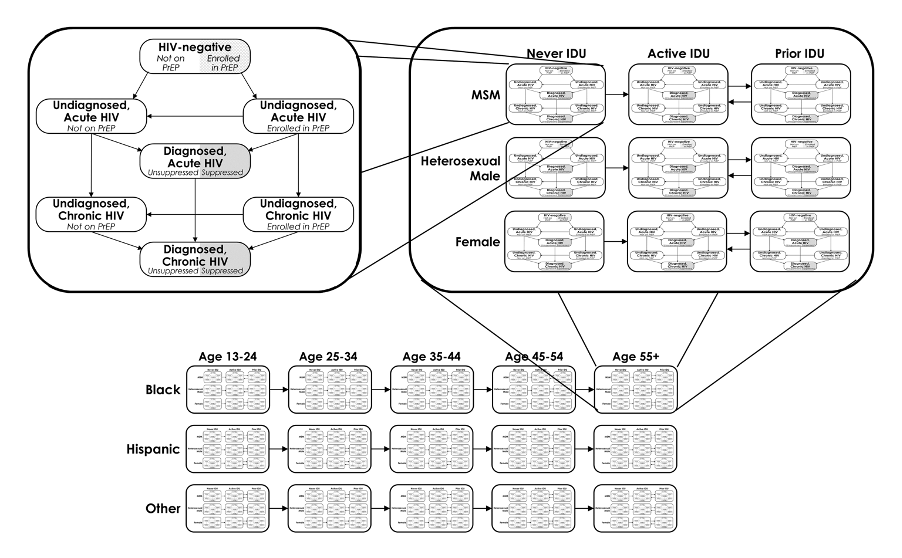
\includegraphics[width=0.75\textwidth]{images/FigureS1}
\end{figure}
The upper left panel shows model populations (compartments) defined by HIV disease state and the continuum of care. Each uninfected population has a proportion who are enrolled in a PrEP program. As people in the model become infected, they first enter the acute HIV phase ? which lasts 2.9 months ? where transmissibility is high, before progressing to chronic HIV. People who become infected with HIV while enrolled in a PrEP program are diagnosed at an average rate of once every 3 months. People with HIV (PWH) who are unaware of their diagnosis and not in a PrEP program are diagnosed according to testing rates that depend on their age, race/ethnicity, sex/sexual behavior, IV drug use (IDU) status, location, and calendar year. All populations of PWH who are aware of their diagnosis have a proportion who are virally suppressed and do not transmit HIV. Each population is further stratified by sex/sexual behavior and IV drug use status (top right), and by age and race/ethnicity (bottom) (Adapted from Fojo et al., 2021 \cite{fojo2021}). All interventions presented in this study are focused on the MSM subgroups. 


\begin{figure}[H]
	\centering
	\caption{Impact of Efficacy and Persistence for Oral and Long-Acting Injectable PrEP on Projected Reduction in HIV Incidence among MSM}
	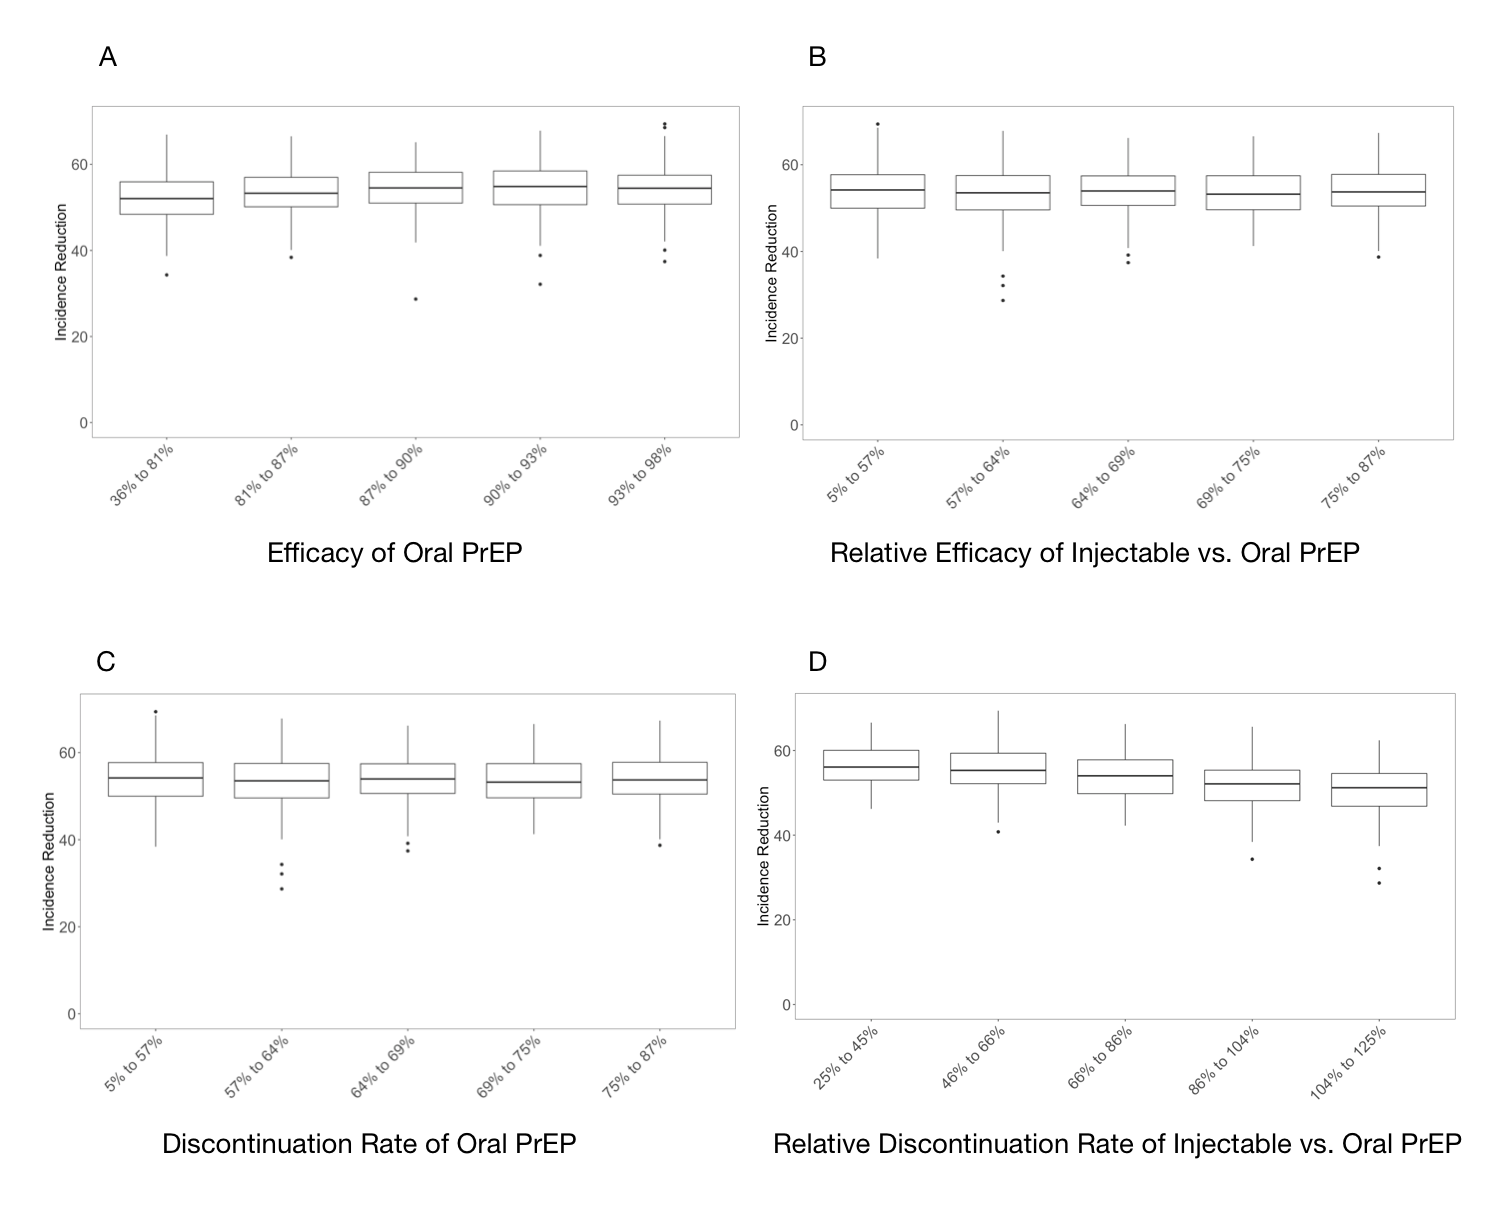
\includegraphics[width=0.75\textwidth]{images/FigureS2}
\end{figure}

For each of the 1,000 simulations per city, we calculated the reduction in total incidence among MSM from 2020 to 2030 across all 32 cities for the 25\% additional uptake of LAI with a baseline of oral PrEP intervention. For each of the four parameters governing PrEP effects A) efficacy of oral PrEP, B) Relative efficacy of injectable vs oral PrEP, C) Discontinuation rate of oral PrEP, D) Relative discontinuation rate of injectable vs oral PrEP), we divided simulations into five groups of 200 simulations each, from low to high values of each parameter. For each group, we present a boxplot of the distribution in incidence reduction: the horizontal line represents the median reduction, the box represents the interquartile range, the whiskers represent the 95\% credible interval, and dots represent outliers. 

\begin{figure}[H]
	\centering
	\caption{Differences Between Projected and Observed Reported Diagnoses among MSM, 2010-2018}
	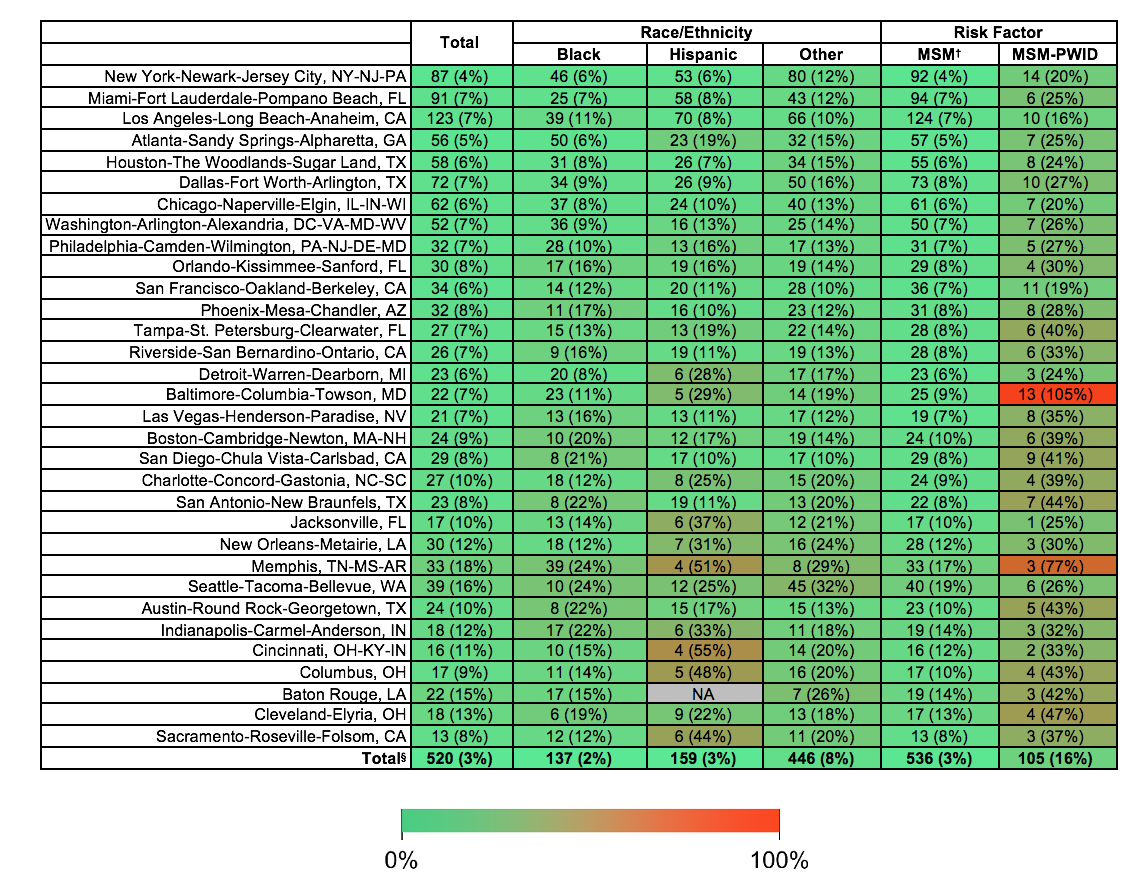
\includegraphics[width=0.75\textwidth]{images/FigureS3}
\end{figure}


The top number in each cell represents the mean, across 1,000 simulations and 9 years (2010-2018), of the absolute value of the difference between projected and observed diagnoses among MSM. The number in parentheses is the mean absolute percent error. \dag MSM = men who have sex with men who do not inject drugs. MSM+PWID = men who have sex with men who are also people who inject drugs. Total = the errors are calculated by subtracting the sum of observed values across MSAs from the sum of projections

\begin{figure}[H]
	\centering
	\caption{Differences Between Projected and Observed Prevalence of Diagnosed HIV among MSM, 2010-2018}
	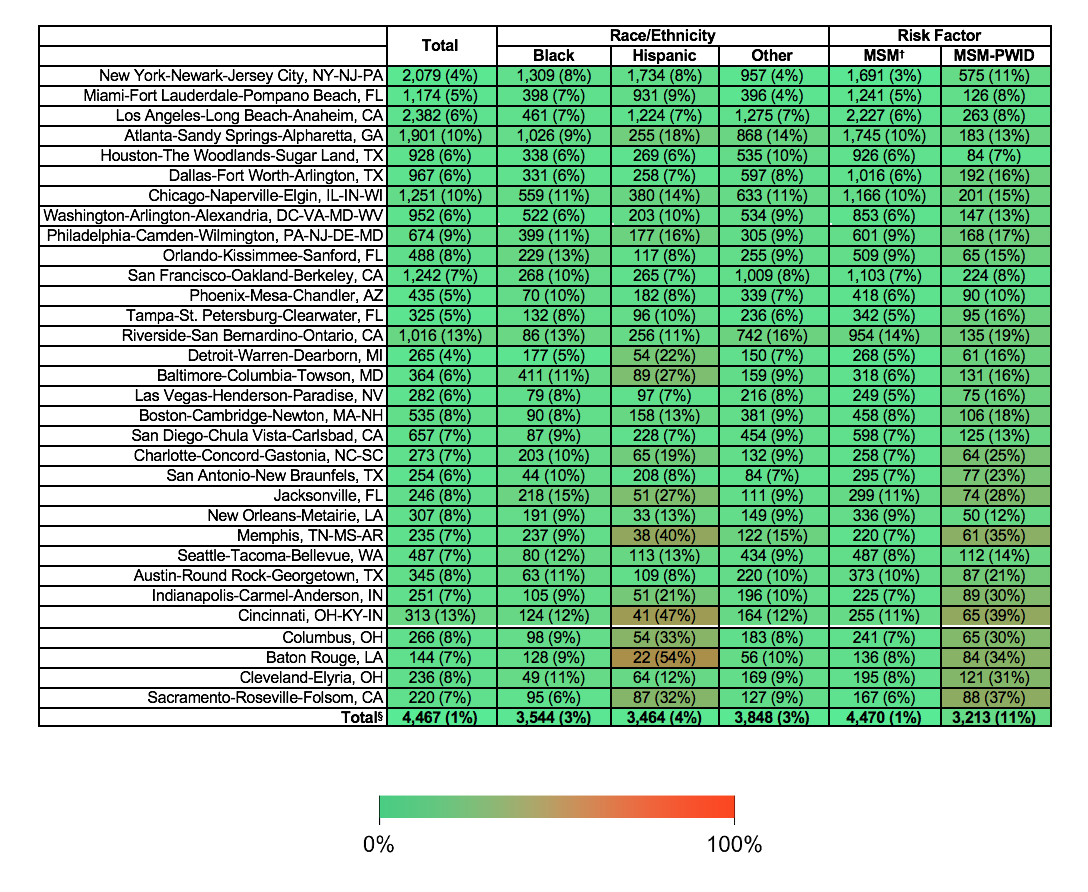
\includegraphics[width=0.75\textwidth]{images/FigureS4}
\end{figure}

The top number in each cell represents the mean, across 1,000 simulations and 9 years (2010-2018), of the absolute value of the difference between projected and observed prevalence of diagnosed HIV. The number in parentheses is the mean absolute percent error. \dag MSM = men who have sex with men who do not inject drugs. MSM+PWID = men who have sex with men who are also people who inject drugs.Total = the errors are calculated by subtracting the sum of observed values across MSAs from the sum of projections.


\begin{figure}[H]
	\centering
	\caption{Ratio of Incident Cases per Population Black MSM vs Non Black Non-Hispanic MSM }
	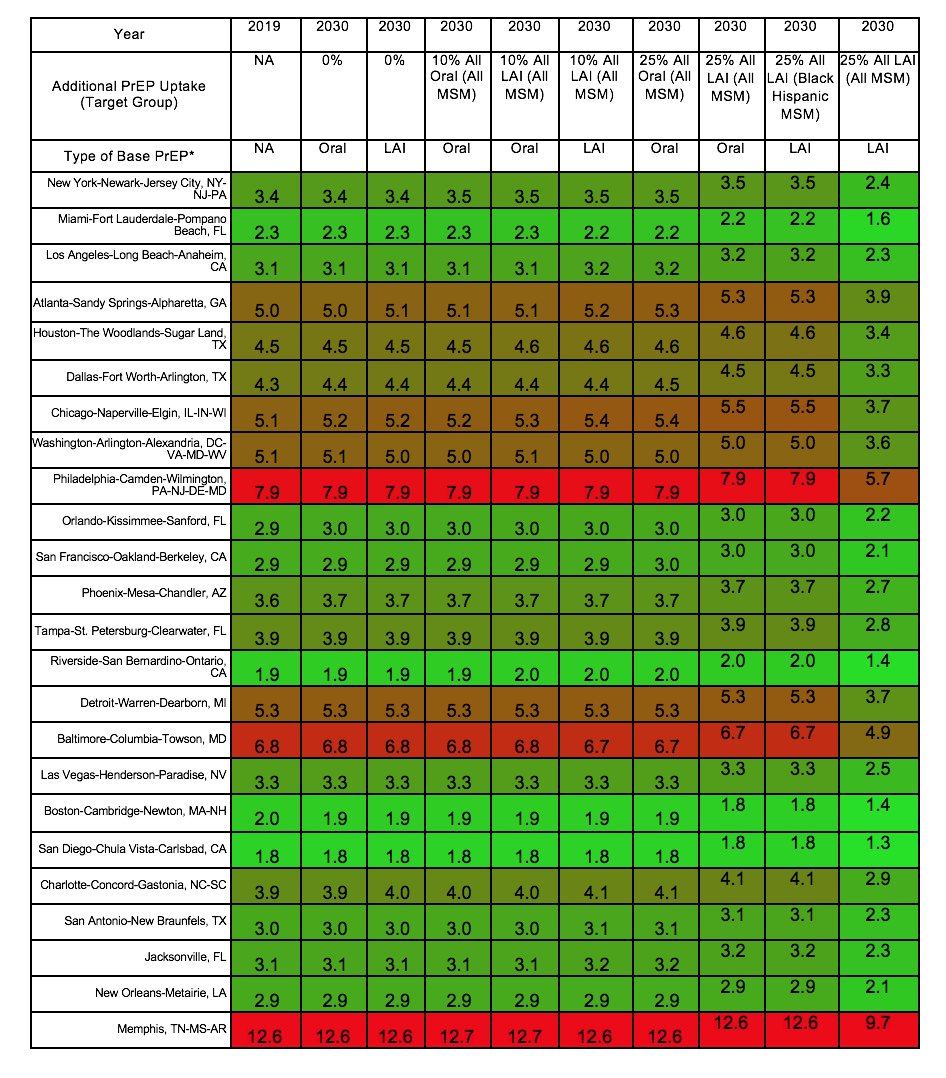
\includegraphics[width=0.75\textwidth]{images/FigureS5_1}

\end{figure}

\pagebreak

\begin{figure}[H]
	\centering
	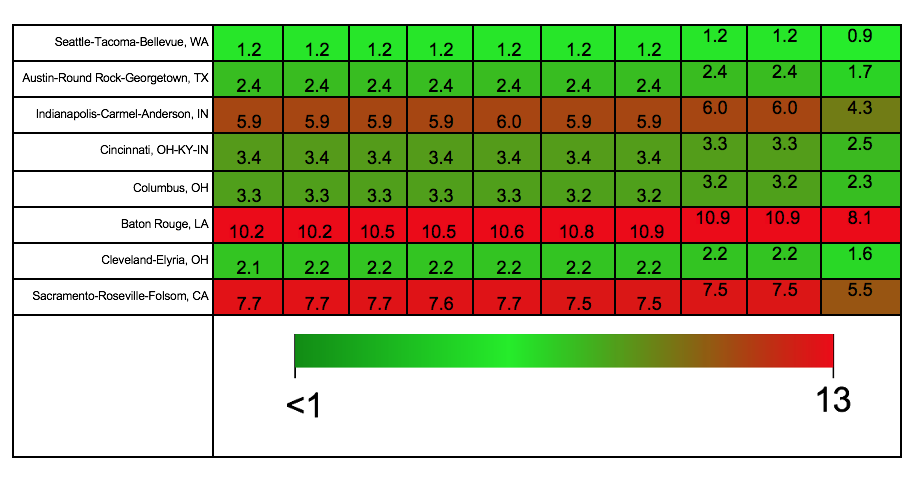
\includegraphics[width=0.75\textwidth]{images/FigureS5_2}
\end{figure}

Each cell shows the ratio of incident HIV cases per population between Black MSM and non-black non-Hispanic MSM for a given intervention and year. The ratio value in each cell represents the mean across 1,000 simulations, with ratios ranging from <1 to 13. 

\begin{figure}[H]
	\centering
	\caption{Ratio of Incident Cases per Population Hispanic MSM vs Non Black Non-Hispanic MSM}
	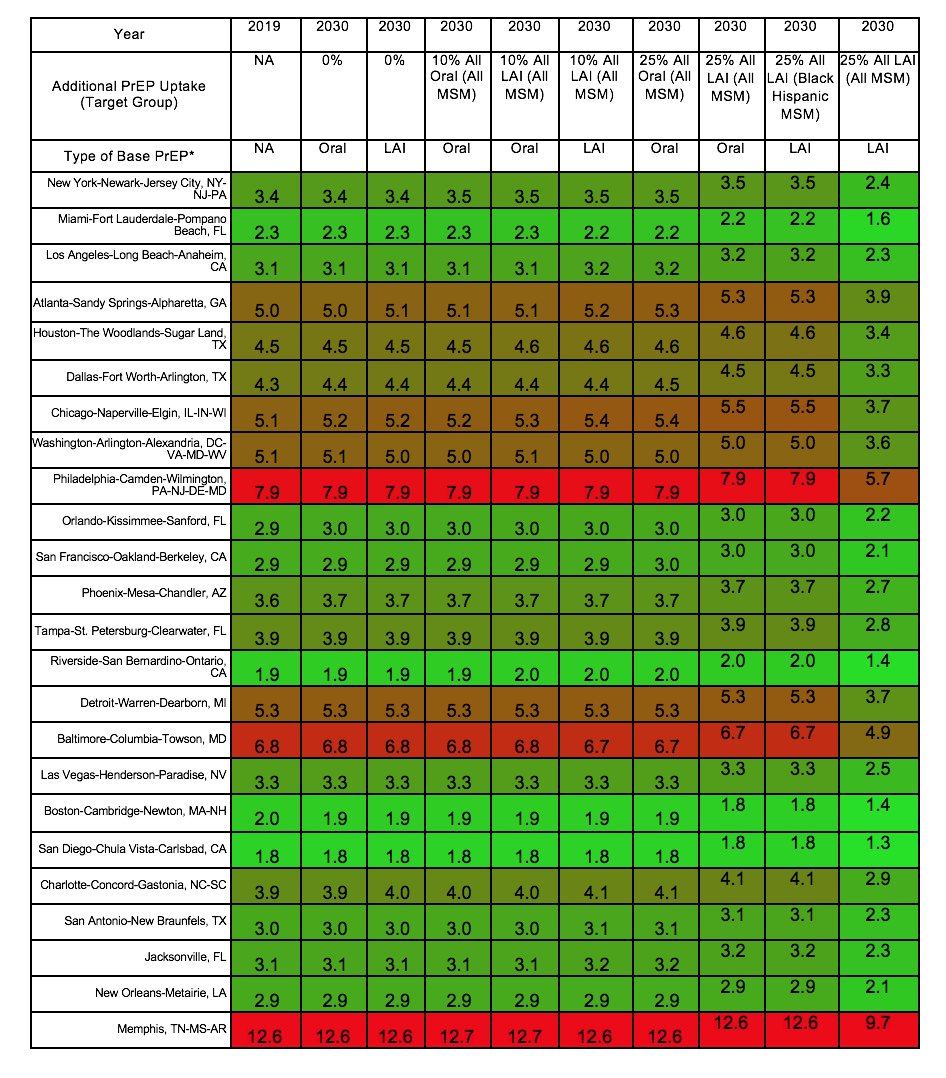
\includegraphics[width=0.75\textwidth]{images/FigureS6_1}
\end{figure}

\pagebreak

\begin{figure}[H]
	\centering
	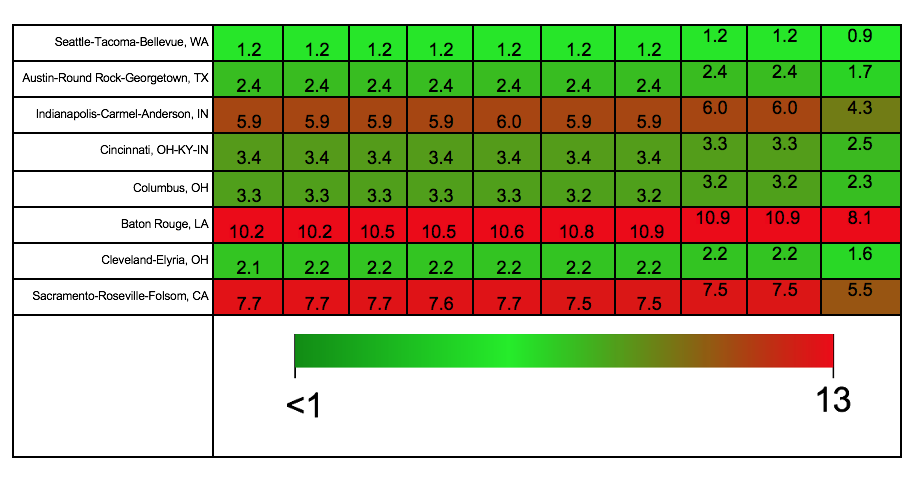
\includegraphics[width=0.75\textwidth]{images/FigureS6_2}
\end{figure}

Each cell shows the ratio of incident HIV cases per population between Hispanic MSM and non-black non-Hispanic MSM for a given intervention and year. The ratio value in each cell represents the mean across 1,000 simulations, with ratios ranging from <1 to 13. 

\begin{figure}[H]
	\centering
	\caption{Relationship Between Incidence Reduction and Aspects of the Underlying HIV Epidemic}
	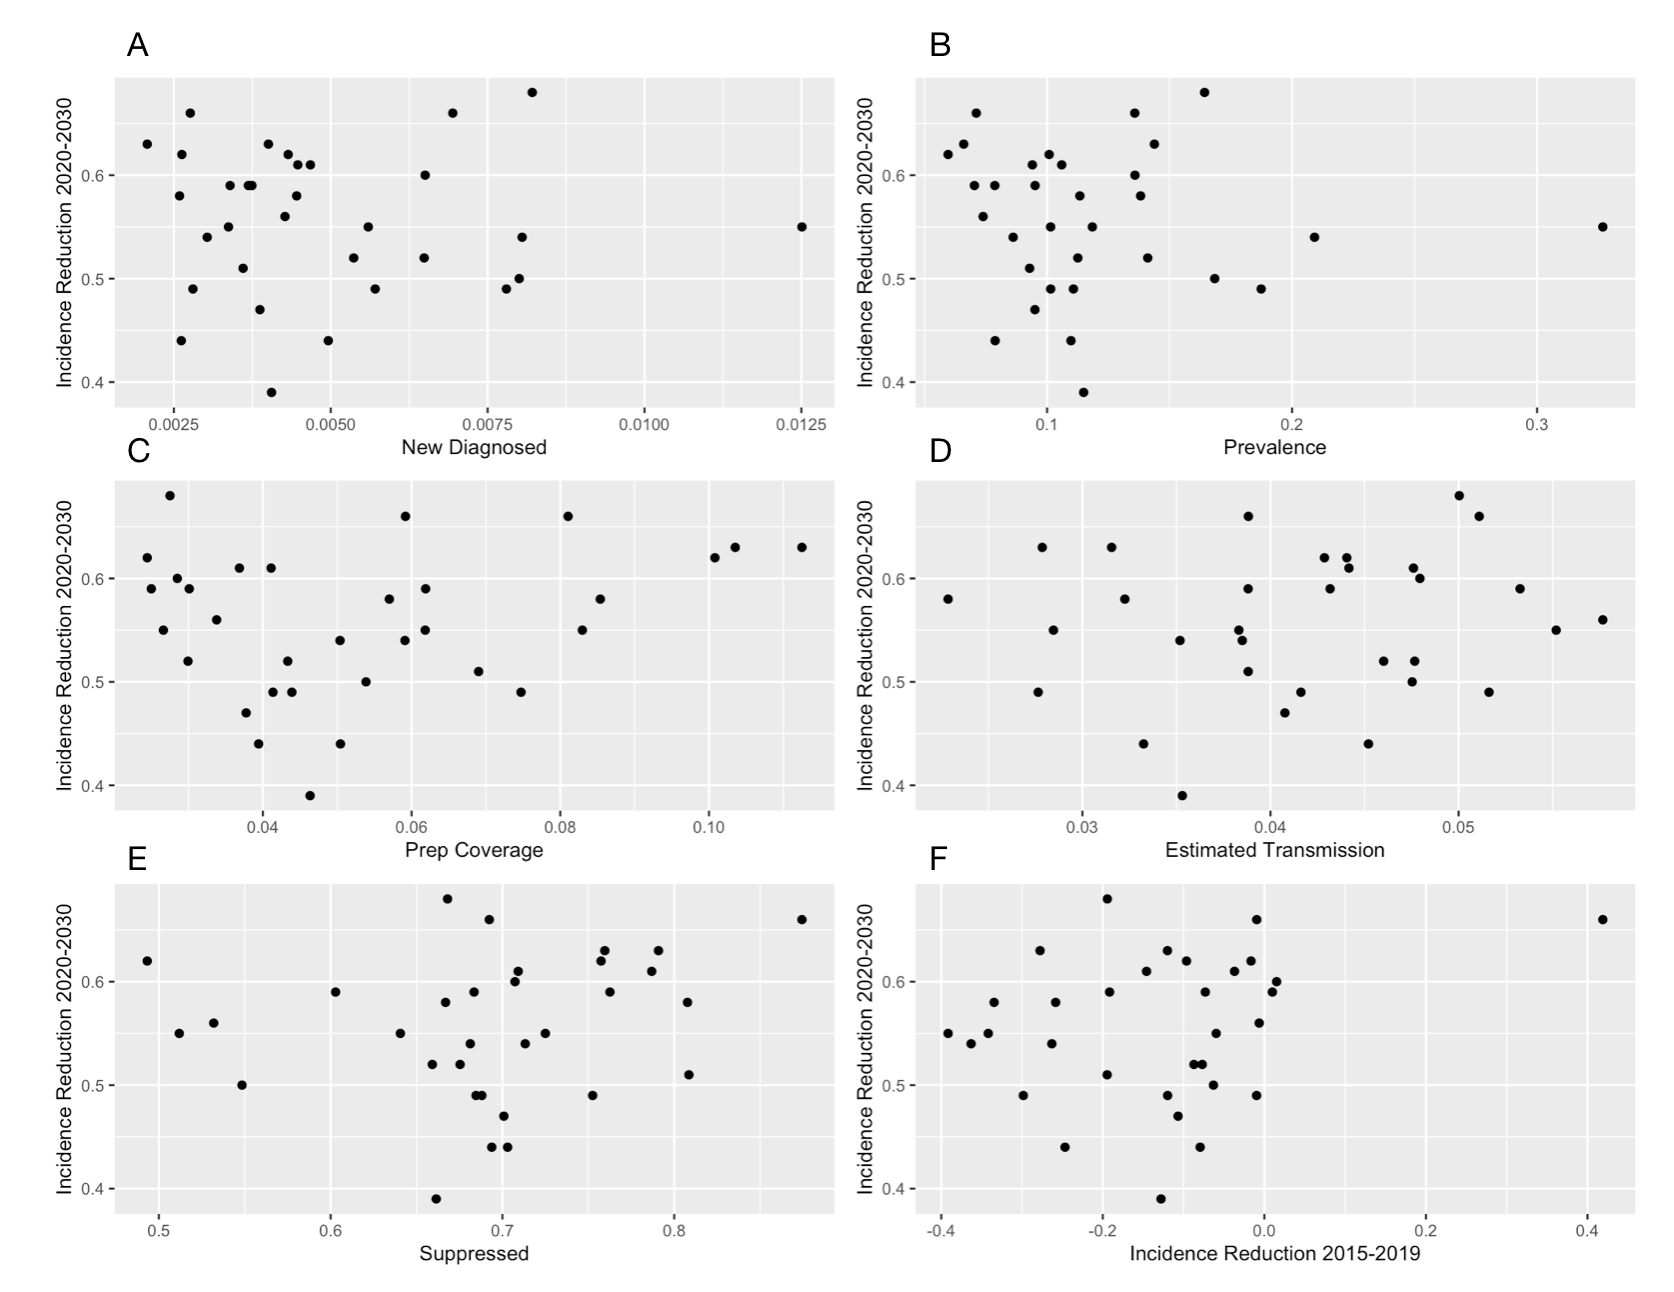
\includegraphics[width=0.75\textwidth]{images/FigureS7}
\end{figure}

Scatterplot of the relationship between variables underlying the HIV epidemic including A)  The number of newly diagnosed patients per population B) The prevalence of HIV per population C) Base PrEP coverage D) The ratio of newly diagnosed patients to HIV prevalence (Estimated Transmission) E) The proportion of virally suppressed individuals F) The incidence reduction between 2015-2019 on the incidence reduction between 2020-2030. Each individual point represents the average for each variables across all 1000 simulations for an individual MSA. 

%---------------------------------%
%-- PARAMETERS --%
%---------------------------------%
\newpage
\section{Model Parameters and Their Prior Distributions}
\tabulinesep=2pt

%\begin{longtable}{| p{.45\textwidth} | c{.09\textwidth} | p{.13\textwidth} | p{.08\textwidth} | p{.25\textwidth} |}
\begin{longtabu} to \textwidth {|X[45,l,m]|X[9,c,m]|X[13,c,m]|X[8,c,m]|X[25,l,m]|}

%-- TABLE SET-UP --%
	\caption{Model Parameters and Sampling Distributions.\label{params_tab}}\\
	
	\hline
%	\multicolumn{2}{| c |}{Table S2: Model Parameters}\\
%	\hline
	\textbf{Parameter} & \textbf{Estimate} & \textbf{Uncertainty Range} & \textbf{Symbol/ Section} & \textbf{References} \\
	\hline
	\hline
	\endfirsthead
	
	\hline
	\multicolumn{5}{|l|}{Table \ref{params_tab} (Model Parameters) continued}\\
	\hline
	\textbf{Parameter} & \textbf{Estimate} & \textbf{Uncertainty Range} & \textbf{Symbol/ Section} & \textbf{References} \\
	\hline
	\hline
	\endhead
	
	\hline
	\hline
	\multicolumn{5}{|l|}{\textit{*Uncertainty Range represents the 95\% confidence interval for a Lognormal distribution unless otherwise indicated}}\\
	\hline
	\endfoot
	
%	\hline
%	\multicolumn{2}{| c |}{End of Table}\\
	\hline\hline
	\endlastfoot
	

%----------------------------%	
%-- HIV TRANSMISSION MULTIPLIERS --% 
%----------------------------%

	\multicolumn{5}{|l|}{\textbf{HIV TRANSMISSION MULTIPLIERS**}}\\ \hline 
		
%	Global Transmission Rate & 1 & \textit{improper uniform on log scale} & $\gamma_0$ (\ref{trates}) & \\ \hline
	
	\multicolumn{5}{|l|}{\textbf{Male-to-male Sexual Transmission}}\\ 
	\multicolumn{5}{|l|}{\textit{(A composite of number of sexual encounters and rate of transmission per encounter)}}\\ \hline
	Black, 2000 & 1 & [0.003 - 354] & $\omega^{(MSM)}$ & \\ \cline{1-3}
	Black, ratio of rate by 2010 to 2000 rate & 1 & [0.257 - 3.891] & \ref{trates} & \\ \cline{1-3}
	Black, ratio of rate by 2020 to 2010 rate & 1 & [0.507 - 1.972] & & \\ \cline{1-3}
	Hispanic, 2000 & 1 & [0.003 - 354] & & \\ \cline{1-3}
	Hispanic, ratio of rate by 2010 to 2000 rate & 1 & [0.257 - 3.891] & & \\ \cline{1-3}
	Hispanic, ratio of rate by 2020 to 2010 rate & 1 & [0.507 - 1.972] & & \\ \cline{1-3}
	Non-Black/Non-Hispanic, 2000 & 1 & [0.003 - 354] & & \\ \cline{1-3}
	Non-Black/Non-Hispanic, ratio of rate by 2010 to 2000 rate & 1 & [0.257 - 3.891] & & \\ \cline{1-3}
	Non-Black/Non-Hispanic, ratio of rate by 2020 to 2010 rate & 1 & [0.507 - 1.972] & & \\ \cline{1-3} \cline{5-5}
	Ratio of rate before 1980 to rate by 2000 (All Races) & 3.1 & [0.404 - 23.790] & & HIV Atlas\cite{hivatlas}\\ \hline
	
	\multicolumn{5}{|l|}{\textbf{Heterosexual Transmission}}\\  
	\multicolumn{5}{|l|}{\textit{(A composite of number of sexual encounters and rate of transmission per encounter)}}\\ \hline
	Black, 2000 & 1 & [0.003 - 354] & $\omega^{(het)}$& \\ \cline{1-3}
	Black, ratio of rate by 2010 to 2000 rate & 1 & [0.257 - 3.891] & \ref{trates} & \\ \cline{1-3}
	Black, ratio of rate by 2020 to 2010 rate & 1 & [0.507 - 1.972] & & \\ \cline{1-3}
	Hispanic, 2000 & 1 & [0.003 - 354] & & \\ \cline{1-3}
	Hispanic, ratio of rate by 2010 to 2000 rate & 1 & [0.257 - 3.891] & & \\ \cline{1-3}
	Hispanic, ratio of rate by 2020 to 2010 rate & 1 & [0.507 - 1.972] & & \\ \cline{1-3}
	Non-Black/Non-Hispanic, 2000 & 1 & [0.003 - 354] & & \\ \cline{1-3}
	Non-Black/Non-Hispanic, ratio of rate by 2010 to 2000 rate & 1 & [0.257 - 3.891] & & \\ \cline{1-3}
	Non-Black/Non-Hispanic, ratio of rate by 2020 to 2010 rate & 1 & [0.507 - 1.972] & & \\ \cline{1-3} \cline{5-5}
	Ratio of rate before 1980 to rate by 2000 (All Races) & 2.2 & [0.287 - 16.883] & & HIV Atlas \cite{hivatlas}\\ \hline
	
	\multicolumn{5}{|l|}{\textbf{Transmission via Needle Sharing}}\\  
	\multicolumn{5}{|l|}{\textit{(A composite of number of needle-sharing encounters and rate of transmission per encounter)}}\\ \hline
	Black & 1 & [0.003 - 354] & $\omega^{(IDU)}$ & \\ \cline{1-3}
	Black, ratio of rate by 2010 to 2000 rate & 1 & [0.257 - 3.891] & \ref{trates} & \\ \cline{1-3}
	Black, ratio of rate by 2020 to 2010 rate & 1 & [0.507 - 1.972] & & \\ \cline{1-3}
	Hispanic & 1 & [0.003 - 354] & & \\ \cline{1-3}
	Hispanic, ratio of rate by 2010 to 2000 rate & 1 & [0.257 - 3.891] & & \\ \cline{1-3}
	Hispanic, ratio of rate by 2020 to 2010 rate & 1 & [0.507 - 1.972] & & \\ \cline{1-3}
	Non-Black/Non-Hispanic, 2000 & 1 & [0.003 - 354] & & \\ \cline{1-3}
	Non-Black/Non-Hispanic, ratio of rate by 2010 to 2000 rate & 1 & [0.257 - 3.891] & & \\ \cline{1-3}
	Non-Black/Non-Hispanic, ratio of rate by 2020 to 2010 rate & 1 & [0.507 - 1.972] & & \\ \cline{1-3} \cline{5-5}
	Ratio of rate before 1980 to rate by 2000 (All Races) & 4.7 & [0.612 - 36.068] & & HIV Atlas\cite{hivatlas}\\ \hline
	

%---------------------------%
%-- SUSCEPTIBILITY BY AGE --%
%---------------------------%

	\multicolumn{5}{|l|}{}\\ 
	\multicolumn{5}{|l|}{}\\ \hline
	\multicolumn{5}{|l|}{\textbf{SUSCEPTIBILTY TO HIV INFECTION BY AGE}}\\ \hline
		
	\multicolumn{5}{|l|}{\textbf{via Male-to-male Sexual Contact}}\\  
	\multicolumn{5}{|l|}{\textit{(A composite of probability of being sexually active, number of encounters, and rate of transmission per encounter)}}\\ \hline
	Age 13-24 prior to 2010 (relative to age 35-44) & 0.67 & [0.48 - 0.94] & $\omega^{(A)}$ & Twenge 2017\cite{twenge2017} \\ \cline{1-3}
	Age 13-24 by 2020 (relative to age 35-44) & 0.67 & [0.48 - 0.94] & (\ref{trates}) &  Abma 2017\cite{abma2017} \\ \cline{1-3}
	Age 25-34 prior to 2010 (relative to age 35-44)	& 1.11 & [0.79 - 1.56] &&\\ \cline{1-3}
	Age 25-34 by 2020 (relative to age 35-44) & 1.11 & [0.79 - 1.56] &&\\ \cline{1-3}
	Age 45-54 (relative to age 35-44) & 0.72 & [0.51 - 1.01] &&\\ \cline{1-3}
	Age 55+ (relative to age 35-44) & 0.35 & [0.25 - 0.49] &&\\ \hline

	\multicolumn{5}{|l|}{\textbf{via Heterosexual Contact}}\\   
	\multicolumn{5}{|l|}{\textit{(A composite of probability of being sexually active, number of encounters, and rate of transmission per encounter)}}\\ \hline
	Age 13-24 (relative to age 35-44) & 0.67 & [0.48 - 0.94] & $\omega^{(A)}$ & Twenge 2017\cite{twenge2017} \\ \cline{1-3}
	Age 25-34 (relative to age 35-44) & 1.11 & [0.79 - 1.56] & (\ref{trates}) & Abma 2017\cite{abma2017} \\ \cline{1-3}
	Age 45-54 (relative to age 35-44) & 0.72 & [0.51 - 1.01] &&	\\ \cline{1-3}
	Age 55+ (relative to age 35-44) & 0.35 & [0.25 - 0.49] &&\\ \hline	

	\multicolumn{5}{|l|}{\textbf{via Needle Sharing}}\\   
	\multicolumn{5}{|l|}{\textit{(A composite of number of needle-sharing encounters and rate of transmission per encounter)}}\\ \hline
	Age 13-24 (relative to age 35-44) & 1.04 & [0.74 - 1.46] & $\omega^{(A)}$ & HIV Surveillance \#24\cite{nhbs24}\\ \cline{1-3}
	Age 25-34 (relative to age 35-44) & 1.06 & [0.75 - 1.49] & (\ref{trates}) & \\ \cline{1-3}	
	Age 45-54 (relative to age 35-44) & 0.84 & [0.60 - 1.18] &&\\ \cline{1-3}
	Age 55+ (relative to age 35-44) & 0.70 & [0.50 - 0.98] &&\\ \hline
	
%-----------------------------%
%-- RELATIVE SUSCEPTIBILITY --%
%-----------------------------%

\multicolumn{5}{|l|}{}\\ \hline
\multicolumn{5}{|l|}{\textbf{RELATIVE SUSCEPTIBILITY TO HIV ACQUISITION}}\\ \hline
	
	via needle sharing, MSM-IDU vs heterosexual male prior to 1990 & 3.30 & [1.67 - 6.51] & & Strathdee 1997 \cite{strathdee1997} \\ \cline{1-3}
	via needle sharing, MSM-IDU vs heterosexual male by 2000 & 3.30 & [1.67 - 6.51] & &\\ \cline{1-3}	
	via needle sharing, MSM-IDU vs heterosexual male by 2010 & 3.30 & [1.67 - 6.51] & &\\ \cline{1-3}	
	via needle sharing, MSM-IDU vs heterosexual male by 2020 & 3.30 & [1.67 - 6.51] & &\\ \hline
	via needle sharing, female vs heterosexual male & 1.10 & [0.56 - 2.17] && HIV Surveillance \#24 \cite{nhbs24} \\ \hline
	via heterosexual contact, male vs female & 0.75 & [0.38 - 1.48] && Shah 2016 \cite{shah2016}, NHBS Report \#19 \cite{nhbs19}\\	\hline
	
%----------------------%
%-- TRANSMISSIBILITY --%
%----------------------%

\multicolumn{5}{|l|}{}\\ \hline
\multicolumn{5}{|l|}{\textbf{TRANSMISSIBILITY OF HIV BY HIV NATURAL HISTORY AND CARE/TREATMENT ENGAGEMENT}}\\ \hline

	Relative Risk of Transmission for Acute vs Chronic HIV & 12 & [8.54 - 16.85] & & Shah 2016 \cite{shah2016}\\ \hline
	Relative Risk of Transmission by PWH with diagnosed vs undiagnosed HIV & 0.3 & [0.21 - 0.42] & & Marks 2005 \cite{marks2005}, Marks 2006 \cite{marks2006}\\ \hline
	Relative Risk of Transmission by PWH virally suppressed vs unsuppressed & 0 & \textit{Not Sampled} & & Eisinger 2019 \cite{eisinger2019}\\ \hline
	
%--------------------------%
%-- SEXUAL ASSORTATIVITY --%
%--------------------------%

	\multicolumn{5}{|l|}{}\\ \hline
	\multicolumn{5}{|l|}{\textbf{SEXUAL ASSORTATIVITY}}\\ \hline
	
	Proportion of female sexual partnerships with MSM, relative to the proportion of MSM in the population & 0.0895 & [0.045 - 0.177] & & Pathela 2006 \cite{pathela2006}\\ \hline
	Proportion of heterosexual male partnerships with other males & 0.004 & [0.002 - 0.008] & & Pathela 2006\cite{pathela2006}\\ \hline
	Proportion of non-IDU sexual partnerships with active IDU, relative the the prevalence of active IDU in the population & 0.2 & [0.10 - 0.39] & & Jenness 2010\cite{jenness2010}\\ \hline
	Proportion of Black sexual partnerships with Black partners, relative to the proportion Black in the population & 3.76 & [2.68 - 5.28] & & Bohl 2011\cite{bohl2011}\\ \hline
	Proportion of Hispanic sexual partnerships with Hispanic partners, relative to the proportion Hispanic in the population & 2.19 & [1.56 - 3.08] & & Mutanski 2014 \cite{mutanski2014}\\ \hline
	Proportion of Non-Black/Non-Hispanic sexual partnerships with Non-Black/Non-Hispanic partners, relative to the proportion Other in the population & 1.55 & [1.10 - 2.18] & & Fujimoto 2015 \cite{fujimoto2015}, Hamilton 2015 \cite{hamilton2015}\\ \hline
	Dispersion of age of sexual partnerships & \textit{Sex- and age-specific} & [0.71 - 1.40] $\times$ estimate & & Chow 2016 \cite{chow2016}\\ \hline
	Ratio of proportion of 13yo who are sexually active to 20-24yo proportion & 0.101 & \textit{Not Sampled} & & Abma 2017 \cite{abma2017}\\ \cline{1-3}
	Ratio of proportion of 14yo who are sexually active to 20-24yo proportion & 0.144 & \textit{Not Sampled} & & \\ \cline{1-3}
	Ratio of proportion of 15yo who are sexually active to 20-24yo proportion & 0.173 & \textit{Not Sampled} & & \\ \cline{1-3}
	Ratio of proportion of 16yo who are sexually active to 20-24yo proportion & 0.346 & \textit{Not Sampled} & & \\ \cline{1-3}
	Ratio of proportion of 17yo who are sexually active to 20-24yo proportion & 0.546 & \textit{Not Sampled} & & \\ \cline{1-3} 
	Ratio of proportion of 18yo who are sexually active to 20-24yo proportion & 0.733 & \textit{Not Sampled} & & \\ \cline{1-3} 
	Ratio of proportion of 19yo who are sexually active to 20-24yo proportion & 0.906 & \textit{Not Sampled} & & \\ \hline
	Ratio of proportion of 65-74yo who are sexually active to 55-64yo proportion & 0.721 & \textit{Not Sampled} & & Lindau 2007 \cite{lindau2007}\\ \cline{1-3} 
	Ratio of proportion of 75+yo who are sexually active to 55-64yo proportion & 0.366 & \textit{Not Sampled} & & \\ \hline

%----------------------------------%
%-- NEEDLE SHARING ASSORTATIVITY --%
%----------------------------------%

	\multicolumn{5}{|l|}{}\\ \hline
	\multicolumn{5}{|l|}{\textbf{NEEDLE SHARING ASSORTATIVITY}}\\ \hline
	
	Proportion of Black needle-sharing partnerships with Black partners, relative to the proportion Black in the population & 9.12 & \textit{Not Sampled} & & Smith 2018 \cite{smith2018}\\ \cline{1-3}
	Proportion of Hispanic needle-sharing partnerships with Hispanic partners, relative to the proportion Hispanic in the population & 1.05 & \textit{Not Sampled} & & \\ \cline{1-3}
	Proportion of Non-Black/Non-Hispanic needle-sharing partnerships with Non-Black/Non-Hispanic partners, relative to the proportion of Non-Black/Non-Hispanic in the population & 1.05 & \textit{Not Sampled} & & \\ \cline{1-3} \cline{5-5}
	Proportion of MSM needle-sharing partnerships with MSM partners, relative to the proportion MSM in the population & 5.29 & \textit{Not Sampled} & & Glick 2018 \cite{glick2018}\\ \cline{1-3}
	Proportion of heterosexual male needle-sharing partnerships with heterosexual male partners, relative to the proportion heterosexual males in the population & 0.82 & \textit{Not Sampled} & & \\ \cline{1-3}
	Proportion of female needle-sharing partnerships with female partners, relative to the proportion female in the population & 0.51 & \textit{Not Sampled} & & \\ \cline{1-3} \cline{5-5}
	Dispersion of age of sexual partnerships & Estimated based on sex and age & \textit{Not Sampled} & & Smith 2018 \cite{smith2018}\\ \cline{1-3} \cline{5-5}
	Ratio of proportion of 13-14yo who share injection equipment to 19-24yo proportion & 0.02 & \textit{Not Sampled} & & \\ \cline{1-3}
	Ratio of proportion of 15-18yo who share injection equipment to 19-24yo proportion & 0.18 & \textit{Not Sampled} & & NSDUH 2015-2018 \cite{nsduh}\\ \cline{1-3} \cline{5-5}
	Ratio of proportion of 65+ yo who share injection equipment to 55-64yo proportion & 0.193 & \textit{Not Sampled} & & NSDUH 2015 and 2016 \cite{nsduh}\\ \hline


%-----------------%
%-- HIV TESTING --%
%-----------------%

	\multicolumn{5}{|l|}{}\\ \hline
	\multicolumn{5}{|l|}{\textbf{PROBABILITY OF RECEIVING HIV TEST WITHIN PAST YEAR}}\\ \hline
	
	MSM, 2010 Odds & 0.67 & [0.17 - 2.61] &$\beta$ (\ref{testing})& NHBS 2011-2018 \cite{nhbs8,nhbs11,nhbs13,nhbs15,nhbs18,nhbs19,nhbs22,nhbs24}\\ \cline{1-3}
	MSM, OR for every year after 2010 & 1.133 & [0.989 - 1.298] && BRFSS 2013-2017 \cite{brfss.13.17} \\ \cline{1-3}
	Heterosexual, 2010 Odds & 0.148 & [0.04 - 0.58] & & \\ \cline{1-3}
	Heterosexual, OR for every year after 2010 & 1.063 & [0.928 - 1.218] & & \\ \cline{1-3}
	IDU, 2010 Odds & 0.369 & [0.09 - 1.44] & & \\ \cline{1-3}
	IDU, OR for every year after 2010 & 1.03 & [0.899 - 1.180] & & \\ \cline{1-3}
	MSM-IDU, 2010 Odds & 0.67 & [0.17 - 2.61] & & \\ \cline{1-3}
	MSM-IDU, OR for every year after 2010 & 1.133 & [0.989 - 1.298] & & \\ \cline{1-3}
	Black vs Non-Black/Non-Hispanic, OR 2010 & 1.215 & [0.31 - 4.73] & & \\ \cline{1-3}
	Black vs Non-Black/Non-Hispanic, OR for every year after 2010 & 1.005 & \textit{Not Sampled} & & \\ \cline{1-3}
	Hispanic vs Non-Black/Non-Hispanic, OR 2010 & 0.853 & [0.22 - 3.32] & & \\ \cline{1-3}
	Hispanic vs Non-Black/Non-Hispanic, OR for every year after 2010 & 1.015 & \textit{Not Sampled} & & \\ \cline{1-3}
	Age 13-24 vs Age 35-44, OR 2010 & 1.267 & [0.33 - 4.93] & & \\ \cline{1-3}
	Age 13-24 vs Age 35-44, OR for every year after 2010 & 0.971 & \textit{Not Sampled} & & \\ \cline{1-3}
	Age 25-34 vs Age 35-44, OR 2010 & 1.345 & [0.35 - 5.23] & & \\ \cline{1-3}
	Age 25-34 vs Age 35-44, OR for every year after 2010 & 0.983 & \textit{Not Sampled} & & \\ \cline{1-3}
	Age 45-54 vs Age 35-44, OR 2010 & 0.836 & [0.21 - 3.25] & & \\ \cline{1-3}
	Age 45-54 vs Age 35-44, OR for every year after 2010 & 0.994 & \textit{Not Sampled} & & \\ \cline{1-3}
	Age 55+  vs Age 35-44, OR 2010 & 0.749 & [0.19 - 2.91] & & \\ \cline{1-3}
	Age 55+ vs Age 35-44, OR for every year after 2010 & 0.991 & \textit{Not Sampled} & & \\ \cline{1-3}
	Female vs Heterosexual Male, OR 2010 & 1.27 & \textit{Not Sampled} & & \\ \cline{1-3}
	Female vs Heterosexual Male OR for every year after 2010 & 0.981 & \textit{Not Sampled} & & \\ \hline
	Relative Probability 1993 vs 2010 & 0.5 & [0.36 - 0.70] & & \\ \hline

%-----------------------%
%-- VIRAL SUPPRESSION --%
%-----------------------%

	\multicolumn{5}{|l|}{}\\ \hline
	\multicolumn{5}{|l|}{\textbf{PROBABILITY OF ACHIEVING VIRAL SUPPRESSION}}\\ \hline
	
	MSM, 2010 Odds & 1.16 & [0.30 - 4.51] & \ref{suppression} & HIV Surveillance \#18-2 \cite{cdc18.2}\\ \cline{1-3}
	MSM, OR for every year after 2010 & 1.17 & [1.021 - 1.340] & & HIV Surveillance \#18-5 \cite{cdc18.5}\\ \cline{1-3}
	Heterosexual, 2010 Odds & 0.885 & [0.23 - 3.44] & & HIV Surveillance \#19-3 \cite{cdc19.3}\\ \cline{1-3}
	Heterosexual, OR for every year after 2010 & 1.149 & [1.003 - 1.316] & & HIV Surveillance \#20-2 \cite{cdc20.2}\\ \cline{1-3}
	IDU, 2010 Odds & 0.703 & [0.18 - 2.74] & & HIV Surveillance \#21-4 \cite{cdc21.4}\\ \cline{1-3}
	IDU, OR for every year after 2010 & 1.143 & [0.998 - 1.309] & & HIV Surveillance \#22-2 \cite{cdc22.2}\\ \cline{1-3}
	MSM-IDU, 2010 Odds & 0.975 & [0.25 - 3.79] & & HIV Surveillance \#23-4 \cite{cdc23.4}\\ \cline{1-3}
	MSM-IDU, OR for every year after 2010 & 1.179 & [1.029 - 1.351] & & HIV Surveillance \#24-3 \cite{cdc24.3}\\ \cline{1-3}
	Black vs. Non-Black/Non-Hispanic, OR 2010 & 0.543 & [0.14 - 2.11] & & HIV Surveillance \#25-2 \cite{cdc25.2}\\ \cline{1-3}
	Black vs. Non-Black/Non-Hispanic, OR for every year after 2010 & 0.997 & [0.870 - 1.142] & & \\ \cline{1-3}
	Hispanic vs. Non-Black/Non-Hispanic, OR 2010 & 0.759 & [0.20 - 2.95] & & \\ \cline{1-3}
	Hispanic vs. Non-Black/Non-Hispanic, OR for every year after 2010 & 0.985 & [0.860 - 1.128] & & \\ \cline{1-3}
	Age 13-24 vs Age 35-44, OR 2010 & 0.531 & [0.14 - 2.07] & & \\ \cline{1-3}
	Age 13-24 vs Age 35-44, OR for every year after 2010 & 1.059 & [0.924 - 1.213] & & \\ \cline{1-3}
	Age 25-34 vs Age 35-44, OR 2010 & 0.73 & [0.19 - 2.84] & & \\ \cline{1-3}
	Age 25-34 vs Age 35-44, OR for every year after 2010 & 1.028 & [0.897 - 1.178] & & \\ \cline{1-3}
	Age 45-54 vs Age 35-44, OR 2010 & 1.194 & [0.31 - 4.65] & & \\ \cline{1-3}
	Age 45-54 vs Age 35-44, OR for every year after 2010 & 1.007 & [0.879 - 1.154] & & \\ \cline{1-3}
	Age 55+  vs Age 35-44, OR 2010 & 1.301 & [0.33 - 5.06] & & \\ \cline{1-3}
	Age 55+ vs Age 35-44, OR for every year after 2010 & 0.999 & [0.872 - 1.144] & & \\ \cline{1-3}
	Female vs Male, Heteroexual, OR 2010 & 1.062 & \textit{Not Sampled} & & \\ \cline{1-3}
	Female vs Male OR, Heterosexual, for every year after 2010 & 1.018 & \textit{Not Sampled} & & \\ \cline{1-3}
	Female vs Male, IDU OR 2010 & 1.154 & \textit{Not Sampled} & & \\ \cline{1-3}
	Female vs Male OR, IDU for every year after 2010 & 1.02 & \textit{Not Sampled} & & \\ \cline{1-3}
	Additional OR for every year after 2020, all subgroups & 1.05 & [1.007 - 1.095] & & \\ \hline
	
%----------%
%-- PrEP --%
%----------%

	\multicolumn{5}{|l|}{}\\ \hline
	\multicolumn{5}{|l|}{\textbf{PrEP COVERAGE AMONG AT-RISK INDIVIDUALS}}\\ \hline
	
	Among Non-Black/Non-Hispanic MSM age 35-44 in 2014, proportion & 0.005 & [0.00 - 0.228]\textsuperscript{†} & & Finlayson 2019\cite{finlayson2019}, Holloway 2017\cite{holloway2017}, HIV Surveillance \#22\cite{nhbs22}\\ \cline{1-3}
	Yearly increase among Non-Black/Non-Hispanic MSM age 35-44 in 2014, proportion & 0.0045 & [0.00 - 0.210]\textsuperscript{†} & & \\ \cline{1-3} \cline{5-5}
	Among Non-Black/Non-Hispanic Heterosexual Men age 35-44 in 2014, proportion & 0.0009 & [0.00 - 0.014]\textsuperscript{†} & & HIV Surveillance \#19\cite{nhbs19}\\ \cline{1-3}
	Yearly increase among Non-Black/Non-Hispanic Heterosexual Men age 35-44 in 2014, proportion & 0.0002 & [0.00 - 0.003]\textsuperscript{†} & & \\ \cline{1-3} \cline{5-5}
	Among Non-Black/Non-Hispanic PWID age 35-44 in 2014, proportion & 0.0001 & [0.00 - 0.002]† & & HIV Surveillance \#24\cite{nhbs24}\\ \cline{1-3}
	Yearly increase among Non-Black/Non-Hispanic PWID age 35-44 in 2014, proportion & 0.0002 & [0.00 - 0.003]\textsuperscript{†} & & \\ \cline{1-3} \cline{5-5}
	Odds ratio of 2014 Coverage, Black vs. Non-Black/Non-Hispanic & 0.5203 & [0.336 - 0.806] & & Finlayson 2019\cite{finlayson2019}\\ \cline{1-3}
	Odds ratio of Yearly Increase Black vs. Non-Black/Non-Hispanic & 0.6559 & [0.424 - 1.016] & & Holloway 2017\cite{holloway2017}\\ \cline{1-3}
	Odds ratio of 2014 Coverage, Hispanic vs. Non-Black/Non-Hispanic & 0.4133 & [0.267 - 0.640] & & HIV Surveillance \#22\cite{nhbs22}\\ \cline{1-3}
	Odds ratio of Yearly Increase Hispanic vs. Non-Black/Non-Hispanic & 0.7675 & [0.496 - 1.189] & & \\ \cline{1-3} \cline{5-5}
	Odds ratio of 2014 Coverage and Yearly Increase, age 13-24 vs 35-44 & 0.6886 & [0.177 - 2.679] & & HIV Surveillance \#24\cite{nhbs24}\\ \cline{1-3}
	Odds ratio of 2014 Coverage and Yearly Increase, age 25-34 vs 35-44 & 1.1511 & [0.296 - 4.478] & & HIV Surveillance \#22\cite{nhbs22}\\ \cline{1-3}
	Odds ratio of 2014 Coverage and Yearly Increase, age 45-54 vs 35-44 & 0.6217 & [0.160 - 2.419] & & \\ \cline{1-3}
	Odds ratio of 2014 Coverage and Yearly Increase, age 55+ vs 35-44 & 0.2048 & [0.053 - 0.797] & & \\ \cline{1-3} \cline{5-5}
	Odds ratio of 2014 Coverage and Yearly Increase, Female vs. Male & 1.5411 & \textit{Not Sampled} & & HIV Surveillance \#24\cite{nhbs24}, HIV Surveillance \#22\cite{nhbs22}\\ \cline{1-3} \cline{5-5}
	Adherence to PrEP & 0.56 & \textit{Not sampled} & & Coy 2019\cite{coy2019}\\ \cline{1-3} \cline{5-5}
	Relative risk of acquiring HIV, PrEP vs no PrEP, male-to-male sexual contact & 0.14 & \textit{Not sampled} & & McCormack 2016\cite{mccormack2016}\\ \cline{1-3} \cline{5-5}
	Relative risk of acquiring HIV, PrEP vs no PrEP, heterosexual contact & 0.25 & \textit{Not sampled} & & Baeten 2012\cite{baeten2012}\\ \cline{1-3} \cline{5-5}
	Relative risk of acquiring HIV, PrEP vs no PrEP, needle-sharing & 0.51 & \textit{Not sampled} & & Choopanya 2013\cite{choopanya2013}\\ \cline{1-3} \cline{5-5}
	Frequency of HIV Screening while on PrEP & 3mo & \textit{Not sampled} & & \\ \hline

%-----------------------%
%-- MSM IN POPULATION --%
%-----------------------%

	\multicolumn{5}{|l|}{}\\ \hline
	\multicolumn{5}{|l|}{\textbf{DISTRIBUTION OF MSM IN THE POPULATION}}\\ \hline
	
	Total Proportion of Males who are MSM & \textit{Location-specific} & [0.84 - 1.19] $\times$ estimate & & Grey 2016 \cite{grey2016}\\ \hline
	Relative Proportion of Males who are MSM, Black vs. Non-Black/Non-Hispanic & 1.28 & \textit{Not Sampled} & & Lansky 2015 \cite{lansky2015}\\ \cline{1-3}
	Relative Proportion of Males who are MSM, Hispanic vs. Non-Black/Non-Hispanic & 0.96 & \textit{Not Sampled} & & \\ \hline

%-------------------%	
%-- HIV MORTALITY --%
%-------------------%

	\multicolumn{5}{|l|}{}\\ \hline
	\multicolumn{5}{|l|}{\textbf{MORTALITY OF UNSUPPRESSED HIV}}\\ \hline
	
	Excess mortality rate among PWH with unsuppressed HIV before 1994 & 0.15 & [0.71 - 1.40] & $\theta^{(HIV})$ & Bhaskaran 2008 \cite{bhaskaran2008}\\ \cline{1-3}
	Excess mortality rate among PWH with unsuppressed HIV by 2000 & 0.036 & [0.026 - 0.051] & (\ref{mortality}) & \\ \cline{1-3}
	Excess mortality rate among PWH with unsuppressed HIV by 2010 & 0.023 & [0.016 - 0.032] & & \\ \hline


	
%-----------------%
%-- AGING RATES --%
%-----------------%
	
	\multicolumn{5}{|l|}{}\\ \hline
	\multicolumn{5}{|l|}{\textbf{PROPORTION IN AGE BRACKET WHO WILL AGE UP TO NEXT BRACKET, per year}}\\ \hline
	
	\multicolumn{5}{|l|}{\textbf{MSM and MSM-IDU}}\\ \hline
	Age 13-24 & 0.27 & [0.19 - 0.38] & $\alpha^{(H)}$ &	HIV Surveillance \#24-5 \cite{cdc24.5} \\ \cline{1-3} \cline{5-5}
	Age 25-34 prior to 2000	& 0.18 & [0.09 - 0.36] & (\ref{aging}) & HIV Surveillance \#14 \cite{cdc14} \\ \cline{1-3} \cline{5-5}
	Age 25-34 after 2010 & 0.13 & [0.07 - 0.26] && HIV Surveillance \#23 \cite{cdc23}\\ \cline{1-3} \cline{5-5}
	Age 35-44 prior to 2000 & 0.10 & \textit{Not Sampled} && \\ \cline{1-3}	 \cline{5-5}
	Age 35-44 after 2010 & 0.14 & [0.07 - 0.28]	&& HIV Surveillance \#23 \cite{cdc23}\\ \cline{1-3} \cline{5-5}
	Age 45-54 prior to 2000 & 0.10 & \textit{Not Sampled} && \\ \cline{1-3} \cline{5-5}
	Age 45-54 after 2010 & 0.08 & \textit{Not Sampled} && \\ \hline
	
	\multicolumn{5}{|l|}{\textbf{Heterosexual}}\\ \hline
	Age 13-24 & 0.25 & [0.18 - 0.35] & $\alpha^{(H)}$ &	HIV Surveillance \#24-5 \cite{cdc24.5} \\ \cline{1-3} \cline{5-5}
	Age 25-34 prior to 2000	& 0.18 & [0.09 - 0.36] & (\ref{aging}) & HIV Surveillance \#14 \cite{cdc14} \\ \cline{1-3} \cline{5-5}
	Age 25-34 after 2010 & 0.13 & [0.07 - 0.26] && HIV Surveillance \#23 \cite{cdc23}\\ \cline{1-3} \cline{5-5}
	Age 35-44 prior to 2000 & 0.10 & \textit{Not Sampled} && \\ \cline{1-3}	 \cline{5-5}
	Age 35-44 after 2010 & 0.14 & [0.07 - 0.28]	&& HIV Surveillance \#23 \cite{cdc23}\\ \cline{1-3} \cline{5-5}
	Age 45-54 prior to 2000 & 0.10 & \textit{Not Sampled} && \\ \cline{1-3} \cline{5-5}
	Age 45-54 after 2010 & 0.08 & \textit{Not Sampled} && \\ \hline
	
	\multicolumn{5}{|l|}{\textbf{PWID}}\\ \hline
	Age 13-24 & 0.32 & [0.23 - 0.45] & $\alpha^{(H)}$ &	HIV Surveillance \#24-5 \cite{cdc24.5} \\ \cline{1-3} \cline{5-5}
	Age 25-34 prior to 2000	& 0.18 & [0.09 - 0.36] & (\ref{aging}) & HIV Surveillance \#14 \cite{cdc14} \\ \cline{1-3} \cline{5-5}
	Age 25-34 after 2010 & 0.13 & [0.07 - 0.26] && HIV Surveillance \#23 \cite{cdc23}\\ \cline{1-3} \cline{5-5}
	Age 35-44 prior to 2000 & 0.10 & \textit{Not Sampled} && \\ \cline{1-3}	 \cline{5-5}
	Age 35-44 after 2010 & 0.14 & [0.07 - 0.28]	&& HIV Surveillance \#23 \cite{cdc23}\\ \cline{1-3} \cline{5-5}
	Age 45-54 prior to 2000 & 0.10 & \textit{Not Sampled} && \\ \cline{1-3} \cline{5-5}
	Age 45-54 after 2010 & 0.08 & \textit{Not Sampled} && \\ \hline


%-----------------%
%-- IV DRUG USE --%
%-----------------%

	\multicolumn{5}{|l|}{}\\ \hline
	\multicolumn{5}{|l|}{\textbf{INJECTION DRUG USE}}\\ \hline
	
	Excess mortality rate among active IDU & 0.0166 & \textit{Not Sampled} & & Mathers 2014 \cite{mathers2014}\\ \hline
	Incidence of IV Drug Use, base estimate & Location- and stratum-specific & - & \ref{idu} & NSDUH 2015-2018 \cite{nsduh} \\ \cline{1-3}
	Multiplier, Incidence of IV Drug Use, Black, before 2000 & 1 & [0.51 - 1.97] & & \\ \cline{1-3}
	Multiplier,Incidence of IV Drug Use, Black, by 2020 & 1 & [0.51 - 1.97] & & \\ \cline{1-3}
	Multiplier,Incidence of IV Drug Use, Hispanic before 2000 & 1 & [0.51 - 1.97] & & \\ \cline{1-3}
	Multiplier,Incidence of IV Drug Use, Hispanic by 2020 & 1 & [0.51 - 1.97] & & \\ \cline{1-3}
	Multiplier,Incidence of IV Drug Use, Non-Black/Non-Hispanic before 2000 & 1 & [0.51 - 1.97] & & \\ \cline{1-3}
	Multiplier,Incidence of IV Drug Use, Non-Black/Non-Hispanic by 2020 & 1 & [0.51 - 1.97] & & \\ \cline{1-3}
	Multiplier,Incidence of IV Drug Use, MSM before 2000 & 1 & [0.51 - 1.97] & & \\ \cline{1-3}
	Multiplier,Incidence of IV Drug Use, MSM by 2020 & 1 & [0.51 - 1.97] & & \\ \cline{1-3}
	Rate of Remission of IV Drug Use & Location- and stratum-specific & [0.51 - 1.97] $\times$ estimate & & \\ \cline{1-3}
	Rate of Relapse of IV Drug Use &  Location- and stratum-specific & [0.51 - 1.97] $\times$ estimate & & \\ \hline

%------------------------%
%-- FUTURE UNCERTAINTY --%
%------------------------%

	\multicolumn{5}{|l|}{}\\ \hline
	\multicolumn{5}{|l|}{\textbf{FUTURE UNCERTAINTY}}\\ \hline
	
	Continued changes in MSM tranmission rates from 2020-2030, as proportion of changes from 2010-2020 & 0.1 & [0.03 - 0.39] & $p_2$ (\ref{logistic_three_point_spline}) & \\ \cline{1-3}
	Continued changes in heterosexual tranmission rates from 2020-2030, as proportion of changes from 2010-2020 & 0.1 & [0.03 - 0.39] &  & \\ \cline{1-3}
	Continued changes in IDU tranmission rates from 2020-2030, as proportion of changes from 2010-2020 & 0.1 & [0.03 - 0.39] & & \\ \hline %\cline{1-3}
	Improvements in testing continue until year & \multicolumn{2}{|c|}{uniform on [2020-2025]} & & \\ \cline{1-3}
	Improvements in viral suppression continue until year & \multicolumn{2}{|c|}{uniform on [2020-2025]} & & \\ \cline{1-3}
	Improvements in PrEP coverage continue until year & \multicolumn{2}{|c|}{uniform on [2020-2025]} & & \\ \hline


\end{longtabu}

 **HIV Transmission Multipliers are relative to the Global Transmission Rate, or the average number of infections generated by one, unsuppressed PWH per year, which is calibrated to match local epidemics

 
%\end{longtable}

%%-------------------------%%
%%-- CALIBRATION TARGETS --%%
%%-------------------------%%

\newpage
\section{Calibration Targets}

\begin{table}[H]
	\caption{Model Calibration Targets}
	\small
	\begin{tabular}{r r c c c}
		\hline
		& \textbf{Target} & \textbf{Years} & \textbf{Level of Stratification} & \textbf{Data Source} \\
		\hline
		\hline
		
		\multirow{3}{*}{1.} & \multirow{3}{*}{Reported diagnoses} & \multirow{3}{*}{2009 to 2017} & sex, age, race, risk factor, & \multirow{3}{*}{CDC MSA reports \cite{hivatlas,msa2010,msa2011,msa2013,msa2014,msa2015,msa2016,cdc24.2} }\\
		& & & sex*age, sex*race, sex*race, & \\
		& & & sex*risk, race*risk & \\
		\hline
		
		\multirow{3}{*}{2.} & \multirow{3}{*}{Estimated number of diagnosed PWH} & \multirow{3}{*}{2008 to 2016} & sex, age, race, and risk factor & \multirow{3}{*}{CDC MSA reports \cite{hivatlas,msa2010,msa2011,msa2013,msa2014,msa2015,msa2016,cdc24.2} }\\
		& & & sex*age, sex*race, sex*race, & \\
		& & & sex*risk, race*risk & \\
		\hline
		
		3. & Mortality in PWH & 2009 to 2016 & sex & CDC MSA reports  \cite{msa2010,msa2011,msa2013,msa2014,msa2015,msa2016,cdc24.2} \\
		\hline
		
		\multirow{2}{*}{4}. & The proportion of PWH aware & \multirow{2}{*}{2010 to 2018} & \multirow{2}{*}{total} & \multirow{2}{*}{HIV Atlas \cite{hivatlas} }\\
		& of their diagnosis (state-level) & & & \\
		\hline
		
		\multirow{2}{*}{5.} & The proportion of diagnosed PWH & \multirow{2}{*}{2010 to 2018} & total + age, race, sex, & \multirow{2}{*}{local health departments} \\
		& who were virally suppressed & & risk factor (when available) & \\
		\hline
		
		\multirow{3}{*}{6.} & The number of individuals & \multirow{3}{*}{2010 to 2018} & \multirow{3}{*}{sex, race} & \multirow{3}{*}{AIDSVu \cite{aidsvu_prep} }\\
		& receiving a prescription for & & & \\
		& emtricitabine/tenofovir for PrEP & & & \\
		\hline
		
		7. & The proportion receiving an HIV test & 2013 to 2017 & age, sex, race & BRFSS \cite{brfss.13.17} \\
		\hline
		
		\multirow{2}{*}{8.} & The prevalence of injection drug use & \multirow{2}{*}{2014 to 2016} & \multirow{2}{*}{age} & \multirow{2}{*}{NSDUH \cite{nsduh} }\\
		& (sub-state estimates) & & & \\
		\hline
		
		9. & Cumulative AIDS mortality & up to 2002 & age, race, sex, risk factor & AIDS Public Information Dataset\cite{apids} \\
		\hline
		
		10. & Reported AIDS diagnoses & 1998 to 2002 & total &  AIDS Public Information Dataset\cite{apids} \\
		\hline		
	\end{tabular}
\end{table}


%%-------------------------%%
%%-- EXTRA RESULT TABLES --%%
%%-------------------------%%

\section{Projected Outcomes Under Different Scenarios for How COVID-19 Pandemic Affects HIV Transmission}


%%-- INCIDENCE --%%

\subsection{Projected Incidence in 2020, 2021, and 2025}

\begin{table}[H]
	\caption{Projected Incidence in 2020 by Metropolitan Statistical Area, Absent Pandemic, Prolonged Barriers to Care, and Rapid Resumption of Care Scenarios}
	\footnotesize
	\begin{tabular}{|r|c|c|c|}
		\hline
		\multirow{2}{*}{\textbf{Location}} & \multirow{2}{*}{\textbf{Absent Pandemic, 2020}} & \textbf{Prolonged Barriers} & \textbf{Rapid Resumption}\\
		&  & \textbf{to Care, 2020} & \textbf{of Care, 2020}\\
		\hline\hline
		New York-Newark-Jersey City, NY-NJ-PA &  2,169 [ 1,883 to  2,446] &  2,183 [ 1,450 to  3,092] &  2,182 [ 1,452 to  3,086]\\
		Miami-Fort Lauderdale-Pompano Beach, FL &  1,680 [ 1,267 to  2,075] &  1,460 [   956 to  2,104] &  1,460 [   955 to  2,103]\\
		Los Angeles-Long Beach-Anaheim, CA &  1,846 [ 1,598 to  2,090] &  1,645 [ 1,136 to  2,230] &  1,645 [ 1,140 to  2,233]\\
		Atlanta-Sandy Springs-Alpharetta, GA &  1,413 [ 1,242 to  1,618] &  1,256 [   904 to  1,697] &  1,256 [   903 to  1,697]\\
		Houston-The Woodlands-Sugar Land, TX &  1,246 [ 1,037 to  1,478] &  1,080 [   755 to  1,496] &  1,080 [   756 to  1,494]\\
		Dallas-Fort Worth-Arlington, TX &  1,108 [   926 to  1,293] &  1,007 [   687 to  1,415] &  1,007 [   687 to  1,415]\\
		Chicago-Naperville-Elgin, IL-IN-WI &  1,123 [   968 to  1,306] &    966 [   676 to  1,311] &    966 [   678 to  1,306]\\
		Washington-Arlington-Alexandria, DC-VA-MD-WV &    565 [   475 to    686] &    555 [   369 to    797] &    555 [   368 to    799]\\
		Philadelphia-Camden-Wilmington, PA-NJ-DE-MD &    564 [   468 to    676] &    512 [   354 to    713] &    511 [   353 to    712]\\
		Orlando-Kissimmee-Sanford, FL &    537 [   430 to    678] &    471 [   313 to    670] &    470 [   312 to    671]\\
		San Francisco-Oakland-Berkeley, CA &    448 [   348 to    565] &    434 [   271 to    642] &    434 [   272 to    637]\\
		Phoenix-Mesa-Chandler, AZ &    444 [   339 to    576] &    393 [   258 to    577] &    392 [   259 to    573]\\
		Tampa-St. Petersburg-Clearwater, FL &    451 [   345 to    605] &    398 [   262 to    578] &    398 [   261 to    578]\\
		Riverside-San Bernardino-Ontario, CA &    495 [   352 to    686] &    427 [   262 to    662] &    427 [   261 to    664]\\
		Detroit-Warren-Dearborn, MI &    416 [   321 to    526] &    377 [   243 to    561] &    377 [   243 to    559]\\
		Baltimore-Columbia-Towson, MD &    265 [   206 to    331] &    249 [   167 to    350] &    249 [   166 to    350]\\
		Las Vegas-Henderson-Paradise, NV &    365 [   296 to    444] &    308 [   208 to    425] &    308 [   208 to    425]\\
		Boston-Cambridge-Newton, MA-NH &    517 [   335 to    809] &    541 [   316 to    846] &    541 [   318 to    850]\\
		San Diego-Chula Vista-Carlsbad, CA &    264 [   209 to    335] &    252 [   162 to    374] &    252 [   161 to    374]\\
		Charlotte-Concord-Gastonia, NC-SC &    313 [   251 to    384] &    275 [   188 to    393] &    275 [   188 to    390]\\
		San Antonio-New Braunfels, TX &    310 [   253 to    380] &    276 [   187 to    403] &    276 [   187 to    403]\\
		Jacksonville, FL &    269 [   197 to    366] &    238 [   152 to    356] &    238 [   151 to    357]\\
		New Orleans-Metairie, LA &    235 [   185 to    295] &    214 [   140 to    305] &    214 [   141 to    307]\\
		Memphis, TN-MS-AR &    235 [   176 to    301] &    209 [   138 to    299] &    209 [   138 to    299]\\
		Seattle-Tacoma-Bellevue, WA &    361 [   219 to    530] &    345 [   182 to    574] &    345 [   182 to    569]\\
		Austin-Round Rock-Georgetown, TX &    208 [   167 to    257] &    193 [   123 to    287] &    193 [   123 to    287]\\
		Indianapolis-Carmel-Anderson, IN &    226 [   179 to    282] &    202 [   134 to    290] &    202 [   134 to    289]\\
		Cincinnati, OH-KY-IN &    319 [   242 to    442] &    298 [   199 to    442] &    297 [   199 to    444]\\
		Columbus, OH &    168 [   127 to    225] &    154 [    99 to    232] &    154 [    99 to    233]\\
		Baton Rouge, LA &    160 [   118 to    224] &    145 [    95 to    212] &    145 [    95 to    212]\\
		Sacramento-Roseville-Folsom, CA &    187 [   140 to    239] &    161 [   103 to    235] &    161 [   104 to    235]\\
		Cleveland-Elyria, OH &    111 [    85 to    141] &    103 [    67 to    151] &    103 [    66 to    151]\\
		\hline
		Total & 19,020 [18,159 to 20,091] & 17,329 [12,411 to 23,467] & 17,321 [12,459 to 23,501]\\
		\hline
	\end{tabular}
\end{table}

\begin{table}[H]
	\caption{Projected Incidence in 2021 by Metropolitan Statistical Area, Absent Pandemic, Prolonged Barriers to Care, and Rapid Resumption of Care Scenarios}
	\footnotesize
	\begin{tabular}{|r|c|c|c|}
		\hline
		\multirow{2}{*}{\textbf{Location}} & \multirow{2}{*}{\textbf{Absent Pandemic, 2021}} & \textbf{Prolonged Barriers} & \textbf{Rapid Resumption}\\
		&  & \textbf{to Care, 2021} & \textbf{of Care, 2021}\\
		\hline\hline
		New York-Newark-Jersey City, NY-NJ-PA &  2,016 [ 1,713 to  2,329] &  2,525 [ 1,651 to  3,571] &  2,098 [ 1,506 to  2,833]\\
		Miami-Fort Lauderdale-Pompano Beach, FL &  1,579 [ 1,137 to  1,999] &  1,605 [ 1,057 to  2,335] &  1,452 [   950 to  2,090]\\
		Los Angeles-Long Beach-Anaheim, CA &  1,786 [ 1,537 to  2,053] &  1,876 [ 1,335 to  2,536] &  1,685 [ 1,232 to  2,223]\\
		Atlanta-Sandy Springs-Alpharetta, GA &  1,375 [ 1,190 to  1,593] &  1,423 [ 1,074 to  1,867] &  1,293 [ 1,010 to  1,658]\\
		Houston-The Woodlands-Sugar Land, TX &  1,202 [   968 to  1,450] &  1,210 [   856 to  1,677] &  1,100 [   791 to  1,503]\\
		Dallas-Fort Worth-Arlington, TX &  1,053 [   859 to  1,245] &  1,146 [   789 to  1,612] &  1,009 [   728 to  1,391]\\
		Chicago-Naperville-Elgin, IL-IN-WI &  1,107 [   941 to  1,304] &  1,095 [   796 to  1,443] &  1,010 [   753 to  1,312]\\
		Washington-Arlington-Alexandria, DC-VA-MD-WV &    506 [   409 to    631] &    623 [   402 to    908] &    520 [   363 to    730]\\
		Philadelphia-Camden-Wilmington, PA-NJ-DE-MD &    530 [   424 to    648] &    568 [   387 to    793] &    505 [   357 to    691]\\
		Orlando-Kissimmee-Sanford, FL &    505 [   396 to    652] &    523 [   349 to    754] &    469 [   325 to    664]\\
		San Francisco-Oakland-Berkeley, CA &    413 [   307 to    540] &    500 [   301 to    766] &    420 [   267 to    613]\\
		Phoenix-Mesa-Chandler, AZ &    415 [   304 to    567] &    436 [   278 to    648] &    388 [   250 to    571]\\
		Tampa-St. Petersburg-Clearwater, FL &    426 [   314 to    605] &    442 [   283 to    654] &    397 [   260 to    584]\\
		Riverside-San Bernardino-Ontario, CA &    476 [   320 to    704] &    487 [   279 to    788] &    431 [   253 to    704]\\
		Detroit-Warren-Dearborn, MI &    395 [   290 to    520] &    437 [   266 to    670] &    378 [   238 to    576]\\
		Baltimore-Columbia-Towson, MD &    239 [   177 to    310] &    273 [   176 to    387] &    235 [   161 to    329]\\
		Las Vegas-Henderson-Paradise, NV &    339 [   267 to    417] &    331 [   228 to    456] &    306 [   210 to    424]\\
		Boston-Cambridge-Newton, MA-NH &    500 [   312 to    794] &    630 [   372 to    971] &    564 [   331 to    876]\\
		San Diego-Chula Vista-Carlsbad, CA &    241 [   189 to    312] &    286 [   179 to    430] &    242 [   159 to    358]\\
		Charlotte-Concord-Gastonia, NC-SC &    303 [   236 to    382] &    312 [   215 to    444] &    280 [   199 to    392]\\
		San Antonio-New Braunfels, TX &    298 [   238 to    374] &    315 [   208 to    469] &    280 [   192 to    408]\\
		Jacksonville, FL &    261 [   181 to    373] &    269 [   169 to    410] &    241 [   153 to    365]\\
		New Orleans-Metairie, LA &    217 [   165 to    282] &    239 [   157 to    345] &    210 [   140 to    294]\\
		Memphis, TN-MS-AR &    220 [   156 to    290] &    232 [   153 to    331] &    206 [   138 to    296]\\
		Seattle-Tacoma-Bellevue, WA &    354 [   197 to    566] &    436 [   202 to    802] &    357 [   174 to    646]\\
		Austin-Round Rock-Georgetown, TX &    191 [   150 to    244] &    222 [   137 to    342] &    188 [   122 to    284]\\
		Indianapolis-Carmel-Anderson, IN &    217 [   167 to    279] &    231 [   151 to    329] &    205 [   138 to    290]\\
		Cincinnati, OH-KY-IN &    314 [   230 to    442] &    331 [   221 to    489] &    311 [   207 to    459]\\
		Columbus, OH &    159 [   116 to    220] &    173 [   113 to    262] &    154 [   101 to    233]\\
		Baton Rouge, LA &    150 [   107 to    218] &    159 [   106 to    234] &    144 [    98 to    209]\\
		Sacramento-Roseville-Folsom, CA &    185 [   134 to    243] &    184 [   111 to    282] &    165 [   103 to    249]\\
		Cleveland-Elyria, OH &     99 [    72 to    132] &    113 [    71 to    168] &     97 [    64 to    145]\\
		\hline
		Total & 18,072 [16,869 to 19,487] & 19,632 [14,136 to 26,582] & 17,342 [13,128 to 22,724]\\
		\hline
	\end{tabular}
\end{table}

\begin{table}[H]
	\caption{Projected Incidence in 2025 by Metropolitan Statistical Area, Absent Pandemic, Prolonged Barriers to Care, and Rapid Resumption of Care Scenarios}
	\footnotesize
	\begin{tabular}{|r|c|c|c|}
		\hline
		\multirow{2}{*}{\textbf{Location}} & \multirow{2}{*}{\textbf{Absent Pandemic, 2025}} & \textbf{Prolonged Barriers} & \textbf{Rapid Resumption}\\
		&  & \textbf{to Care, 2025} & \textbf{of Care, 2025}\\
		\hline\hline
		New York-Newark-Jersey City, NY-NJ-PA &  1,720 [ 1,303 to  2,158] &  1,775 [ 1,338 to  2,277] &  1,732 [ 1,311 to  2,209]\\
		Miami-Fort Lauderdale-Pompano Beach, FL &  1,322 [   813 to  1,862] &  1,347 [   847 to  1,858] &  1,316 [   825 to  1,817]\\
		Los Angeles-Long Beach-Anaheim, CA &  1,656 [ 1,305 to  2,043] &  1,680 [ 1,328 to  2,097] &  1,643 [ 1,311 to  2,029]\\
		Atlanta-Sandy Springs-Alpharetta, GA &  1,314 [ 1,044 to  1,585] &  1,315 [ 1,035 to  1,596] &  1,307 [ 1,024 to  1,582]\\
		Houston-The Woodlands-Sugar Land, TX &  1,112 [   796 to  1,464] &  1,124 [   780 to  1,505] &  1,102 [   766 to  1,467]\\
		Dallas-Fort Worth-Arlington, TX &    935 [   684 to  1,191] &    949 [   691 to  1,203] &    929 [   676 to  1,178]\\
		Chicago-Naperville-Elgin, IL-IN-WI &  1,093 [   861 to  1,366] &  1,092 [   861 to  1,352] &  1,078 [   854 to  1,337]\\
		Washington-Arlington-Alexandria, DC-VA-MD-WV &    398 [   264 to    567] &    410 [   278 to    570] &    401 [   274 to    555]\\
		Philadelphia-Camden-Wilmington, PA-NJ-DE-MD &    457 [   310 to    635] &    462 [   325 to    638] &    454 [   320 to    626]\\
		Orlando-Kissimmee-Sanford, FL &    431 [   295 to    596] &    437 [   296 to    597] &    427 [   286 to    582]\\
		San Francisco-Oakland-Berkeley, CA &    337 [   216 to    505] &    353 [   228 to    530] &    339 [   222 to    500]\\
		Phoenix-Mesa-Chandler, AZ &    356 [   211 to    561] &    361 [   216 to    579] &    352 [   211 to    556]\\
		Tampa-St. Petersburg-Clearwater, FL &    370 [   227 to    609] &    377 [   231 to    606] &    367 [   227 to    586]\\
		Riverside-San Bernardino-Ontario, CA &    433 [   225 to    796] &    442 [   241 to    810] &    423 [   231 to    764]\\
		Detroit-Warren-Dearborn, MI &    358 [   221 to    543] &    372 [   230 to    562] &    357 [   222 to    533]\\
		Baltimore-Columbia-Towson, MD &    189 [   115 to    281] &    192 [   121 to    284] &    189 [   118 to    280]\\
		Las Vegas-Henderson-Paradise, NV &    282 [   187 to    386] &    285 [   190 to    391] &    279 [   186 to    383]\\
		Boston-Cambridge-Newton, MA-NH &    428 [   254 to    681] &    432 [   267 to    678] &    428 [   260 to    674]\\
		San Diego-Chula Vista-Carlsbad, CA &    194 [   134 to    279] &    202 [   138 to    285] &    195 [   133 to    274]\\
		Charlotte-Concord-Gastonia, NC-SC &    287 [   197 to    404] &    291 [   199 to    408] &    284 [   195 to    395]\\
		San Antonio-New Braunfels, TX &    277 [   193 to    375] &    280 [   199 to    382] &    274 [   195 to    370]\\
		Jacksonville, FL &    244 [   144 to    411] &    248 [   147 to    411] &    241 [   144 to    395]\\
		New Orleans-Metairie, LA &    181 [   116 to    261] &    185 [   122 to    265] &    181 [   120 to    259]\\
		Memphis, TN-MS-AR &    190 [   113 to    273] &    192 [   115 to    275] &    189 [   112 to    272]\\
		Seattle-Tacoma-Bellevue, WA &    326 [   135 to    677] &    352 [   146 to    732] &    325 [   139 to    659]\\
		Austin-Round Rock-Georgetown, TX &    154 [   105 to    214] &    161 [   109 to    229] &    155 [   105 to    220]\\
		Indianapolis-Carmel-Anderson, IN &    198 [   132 to    277] &    202 [   130 to    275] &    197 [   128 to    270]\\
		Cincinnati, OH-KY-IN &    297 [   189 to    437] &    302 [   190 to    440] &    298 [   190 to    434]\\
		Columbus, OH &    139 [    90 to    210] &    142 [    91 to    215] &    139 [    89 to    212]\\
		Baton Rouge, LA &    132 [    83 to    210] &    135 [    87 to    204] &    133 [    86 to    202]\\
		Sacramento-Roseville-Folsom, CA &    186 [   114 to    283] &    189 [   117 to    281] &    180 [   112 to    264]\\
		Cleveland-Elyria, OH &     78 [    46 to    118] &     80 [    47 to    121] &     78 [    46 to    119]\\
		
		\hline
		Total & 16,073 [13,150 to 19,076] & 16,362 [13,422 to 19,537] & 15,992 [13,215 to 18,896]\\
		
		\hline
	\end{tabular}
\end{table}


%%-- REPORTED DIAGNOSES --%%

\subsection{Projected Reported Diagnoses in 2020, 2021, and 2025}

\begin{table}[H]
	\caption{Projected Reported Diagnoses in 2020 by Metropolitan Statistical Area, Absent Pandemic, Prolonged Barriers to Care, and Rapid Resumption of Care Scenarios}
	\footnotesize
	\begin{tabular}{|r|c|c|c|}
		\hline
		\multirow{2}{*}{\textbf{Location}} & \multirow{2}{*}{\textbf{Absent Pandemic, 2020}} & \textbf{Prolonged Barriers} & \textbf{Rapid Resumption}\\
		&  & \textbf{to Care, 2020} & \textbf{of Care, 2020}\\
		\hline\hline
		New York-Newark-Jersey City, NY-NJ-PA &  2,492 [ 2,264 to  2,730] &  2,098 [ 1,648 to  2,568] &  2,098 [ 1,647 to  2,564]\\
		Miami-Fort Lauderdale-Pompano Beach, FL &  1,877 [ 1,643 to  2,112] &  1,548 [ 1,206 to  1,928] &  1,548 [ 1,206 to  1,927]\\
		Los Angeles-Long Beach-Anaheim, CA &  1,878 [ 1,659 to  2,097] &  1,549 [ 1,183 to  1,937] &  1,548 [ 1,182 to  1,938]\\
		Atlanta-Sandy Springs-Alpharetta, GA &  1,460 [ 1,308 to  1,634] &  1,208 [   944 to  1,496] &  1,208 [   944 to  1,498]\\
		Houston-The Woodlands-Sugar Land, TX &  1,259 [ 1,124 to  1,418] &  1,036 [   794 to  1,296] &  1,036 [   794 to  1,296]\\
		Dallas-Fort Worth-Arlington, TX &  1,187 [ 1,024 to  1,343] &    983 [   749 to  1,245] &    984 [   749 to  1,245]\\
		Chicago-Naperville-Elgin, IL-IN-WI &  1,131 [ 1,003 to  1,275] &    930 [   728 to  1,152] &    929 [   727 to  1,152]\\
		Washington-Arlington-Alexandria, DC-VA-MD-WV &    721 [   630 to    827] &    608 [   471 to    755] &    608 [   471 to    754]\\
		Philadelphia-Camden-Wilmington, PA-NJ-DE-MD &    651 [   573 to    738] &    542 [   421 to    678] &    542 [   421 to    678]\\
		Orlando-Kissimmee-Sanford, FL &    590 [   501 to    698] &    486 [   361 to    630] &    486 [   361 to    630]\\
		San Francisco-Oakland-Berkeley, CA &    513 [   436 to    607] &    430 [   327 to    550] &    430 [   327 to    550]\\
		Phoenix-Mesa-Chandler, AZ &    501 [   417 to    596] &    414 [   308 to    532] &    414 [   308 to    532]\\
		Tampa-St. Petersburg-Clearwater, FL &    481 [   404 to    574] &    397 [   296 to    514] &    397 [   296 to    513]\\
		Riverside-San Bernardino-Ontario, CA &    512 [   415 to    622] &    420 [   305 to    547] &    420 [   305 to    547]\\
		Detroit-Warren-Dearborn, MI &    418 [   355 to    485] &    346 [   262 to    442] &    346 [   262 to    441]\\
		Baltimore-Columbia-Towson, MD &    338 [   292 to    387] &    283 [   216 to    353] &    283 [   216 to    353]\\
		Las Vegas-Henderson-Paradise, NV &    403 [   346 to    465] &    330 [   252 to    418] &    330 [   252 to    417]\\
		Boston-Cambridge-Newton, MA-NH &    488 [   376 to    650] &    416 [   287 to    587] &    416 [   288 to    586]\\
		San Diego-Chula Vista-Carlsbad, CA &    316 [   263 to    377] &    263 [   195 to    344] &    263 [   195 to    344]\\
		Charlotte-Concord-Gastonia, NC-SC &    319 [   273 to    367] &    262 [   196 to    337] &    262 [   196 to    337]\\
		San Antonio-New Braunfels, TX &    313 [   273 to    361] &    259 [   197 to    326] &    259 [   197 to    326]\\
		Jacksonville, FL &    279 [   234 to    334] &    230 [   172 to    302] &    230 [   172 to    302]\\
		New Orleans-Metairie, LA &    256 [   223 to    292] &    212 [   160 to    266] &    212 [   160 to    266]\\
		Memphis, TN-MS-AR &    274 [   235 to    315] &    226 [   172 to    285] &    226 [   172 to    285]\\
		Seattle-Tacoma-Bellevue, WA &    369 [   263 to    478] &    308 [   207 to    429] &    308 [   208 to    429]\\
		Austin-Round Rock-Georgetown, TX &    228 [   194 to    267] &    190 [   143 to    243] &    190 [   143 to    243]\\
		Indianapolis-Carmel-Anderson, IN &    218 [   183 to    254] &    180 [   136 to    229] &    180 [   136 to    229]\\
		Cincinnati, OH-KY-IN &    270 [   224 to    320] &    223 [   166 to    288] &    223 [   166 to    289]\\
		Columbus, OH &    178 [   149 to    213] &    147 [   111 to    190] &    147 [   111 to    190]\\
		Baton Rouge, LA &    177 [   154 to    209] &    147 [   111 to    190] &    147 [   111 to    190]\\
		Sacramento-Roseville-Folsom, CA &    180 [   144 to    219] &    148 [   111 to    197] &    148 [   110 to    197]\\
		Cleveland-Elyria, OH &    135 [   115 to    158] &    113 [    86 to    142] &    113 [    86 to    142]\\
		\hline
		Total & 20,411 [19,635 to 21,212] & 16,930 [13,517 to 20,306] & 16,930 [13,514 to 20,319]\\
		\hline
	\end{tabular}
\end{table}

\begin{table}[H]
	\caption{Projected Reported Diagnoses in 2021 by Metropolitan Statistical Area, Absent Pandemic, Prolonged Barriers to Care, and Rapid Resumption of Care Scenarios}
	\footnotesize
	\begin{tabular}{|r|c|c|c|}
		\hline
		\multirow{2}{*}{\textbf{Location}} & \multirow{2}{*}{\textbf{Absent Pandemic, 2021}} & \textbf{Prolonged Barriers} & \textbf{Rapid Resumption}\\
		&  & \textbf{to Care, 2021} & \textbf{of Care, 2021}\\
		\hline\hline
		New York-Newark-Jersey City, NY-NJ-PA &  2,307 [ 2,050 to  2,590] &  2,121 [ 1,583 to  2,722] &  2,334 [ 1,908 to  2,834]\\
		Miami-Fort Lauderdale-Pompano Beach, FL &  1,778 [ 1,483 to  2,082] &  1,491 [ 1,133 to  1,897] &  1,673 [ 1,332 to  2,050]\\
		Los Angeles-Long Beach-Anaheim, CA &  1,814 [ 1,574 to  2,067] &  1,533 [ 1,147 to  1,944] &  1,715 [ 1,384 to  2,066]\\
		Atlanta-Sandy Springs-Alpharetta, GA &  1,413 [ 1,252 to  1,594] &  1,215 [   928 to  1,528] &  1,346 [ 1,099 to  1,643]\\
		Houston-The Woodlands-Sugar Land, TX &  1,214 [ 1,048 to  1,403] &  1,009 [   763 to  1,293] &  1,131 [   924 to  1,399]\\
		Dallas-Fort Worth-Arlington, TX &  1,129 [   957 to  1,301] &    978 [   730 to  1,247] &  1,085 [   860 to  1,366]\\
		Chicago-Naperville-Elgin, IL-IN-WI &  1,108 [   968 to  1,266] &    925 [   706 to  1,157] &  1,031 [   824 to  1,271]\\
		Washington-Arlington-Alexandria, DC-VA-MD-WV &    641 [   541 to    753] &    594 [   450 to    775] &    650 [   519 to    824]\\
		Philadelphia-Camden-Wilmington, PA-NJ-DE-MD &    606 [   515 to    708] &    532 [   407 to    686] &    587 [   457 to    739]\\
		Orlando-Kissimmee-Sanford, FL &    562 [   470 to    680] &    475 [   349 to    629] &    529 [   416 to    668]\\
		San Francisco-Oakland-Berkeley, CA &    473 [   389 to    577] &    427 [   311 to    559] &    471 [   363 to    589]\\
		Phoenix-Mesa-Chandler, AZ &    472 [   382 to    581] &    401 [   292 to    537] &    447 [   344 to    572]\\
		Tampa-St. Petersburg-Clearwater, FL &    458 [   373 to    570] &    386 [   283 to    505] &    431 [   336 to    551]\\
		Riverside-San Bernardino-Ontario, CA &    494 [   379 to    626] &    416 [   288 to    569] &    461 [   337 to    622]\\
		Detroit-Warren-Dearborn, MI &    398 [   324 to    482] &    343 [   248 to    453] &    380 [   288 to    493]\\
		Baltimore-Columbia-Towson, MD &    302 [   253 to    357] &    271 [   204 to    345] &    298 [   236 to    373]\\
		Las Vegas-Henderson-Paradise, NV &    380 [   320 to    454] &    313 [   237 to    399] &    352 [   280 to    438]\\
		Boston-Cambridge-Newton, MA-NH &    488 [   350 to    698] &    476 [   315 to    680] &    522 [   356 to    746]\\
		San Diego-Chula Vista-Carlsbad, CA &    289 [   234 to    355] &    255 [   184 to    335] &    283 [   217 to    365]\\
		Charlotte-Concord-Gastonia, NC-SC &    308 [   253 to    366] &    258 [   191 to    341] &    288 [   229 to    364]\\
		San Antonio-New Braunfels, TX &    301 [   255 to    355] &    257 [   190 to    339] &    285 [   223 to    370]\\
		Jacksonville, FL &    269 [   215 to    338] &    228 [   168 to    306] &    254 [   194 to    331]\\
		New Orleans-Metairie, LA &    237 [   200 to    280] &    205 [   149 to    262] &    228 [   183 to    282]\\
		Memphis, TN-MS-AR &    255 [   210 to    302] &    217 [   164 to    279] &    242 [   194 to    307]\\
		Seattle-Tacoma-Bellevue, WA &    368 [   244 to    513] &    337 [   208 to    514] &    366 [   228 to    548]\\
		Austin-Round Rock-Georgetown, TX &    210 [   175 to    251] &    185 [   133 to    248] &    204 [   157 to    261]\\
		Indianapolis-Carmel-Anderson, IN &    209 [   170 to    249] &    178 [   130 to    231] &    198 [   155 to    250]\\
		Cincinnati, OH-KY-IN &    271 [   219 to    340] &    234 [   171 to    303] &    261 [   199 to    336]\\
		Columbus, OH &    167 [   136 to    208] &    144 [   105 to    191] &    160 [   124 to    206]\\
		Baton Rouge, LA &    165 [   137 to    204] &    140 [   103 to    182] &    157 [   128 to    195]\\
		Sacramento-Roseville-Folsom, CA &    177 [   138 to    220] &    146 [   106 to    197] &    163 [   123 to    214]\\
		Cleveland-Elyria, OH &    121 [    99 to    146] &    107 [    79 to    139] &    118 [    91 to    151]\\
		\hline
		Total & 19,383 [18,138 to 20,779] & 16,796 [13,066 to 20,829] & 18,652 [15,740 to 22,065]\\
		\hline
	\end{tabular}
\end{table}

\begin{table}[H]
	\caption{Projected Reported Diagnoses in 2025 by Metropolitan Statistical Area, Absent Pandemic, Prolonged Barriers to Care, and Rapid Resumption of Care Scenarios}
	\footnotesize
	\begin{tabular}{|r|c|c|c|}
		\hline
		\multirow{2}{*}{\textbf{Location}} & \multirow{2}{*}{\textbf{Absent Pandemic, 2025}} & \textbf{Prolonged Barriers} & \textbf{Rapid Resumption}\\
		&  & \textbf{to Care, 2025} & \textbf{of Care, 2025}\\
		\hline\hline
		New York-Newark-Jersey City, NY-NJ-PA &  1,831 [ 1,504 to  2,181] &  1,981 [ 1,585 to  2,477] &  1,884 [ 1,534 to  2,329]\\
		Miami-Fort Lauderdale-Pompano Beach, FL &  1,424 [   981 to  1,804] &  1,488 [ 1,034 to  1,945] &  1,430 [   989 to  1,840]\\
		Los Angeles-Long Beach-Anaheim, CA &  1,624 [ 1,369 to  1,901] &  1,696 [ 1,380 to  2,040] &  1,630 [ 1,346 to  1,941]\\
		Atlanta-Sandy Springs-Alpharetta, GA &  1,284 [ 1,067 to  1,504] &  1,313 [ 1,080 to  1,548] &  1,285 [ 1,053 to  1,512]\\
		Houston-The Woodlands-Sugar Land, TX &  1,078 [   846 to  1,304] &  1,113 [   868 to  1,385] &  1,075 [   844 to  1,338]\\
		Dallas-Fort Worth-Arlington, TX &    935 [   733 to  1,142] &    977 [   750 to  1,207] &    940 [   731 to  1,154]\\
		Chicago-Naperville-Elgin, IL-IN-WI &  1,063 [   878 to  1,281] &  1,084 [   883 to  1,301] &  1,055 [   869 to  1,254]\\
		Washington-Arlington-Alexandria, DC-VA-MD-WV &    448 [   333 to    592] &    483 [   349 to    635] &    461 [   335 to    602]\\
		Philadelphia-Camden-Wilmington, PA-NJ-DE-MD &    484 [   356 to    628] &    503 [   376 to    649] &    486 [   367 to    636]\\
		Orlando-Kissimmee-Sanford, FL &    453 [   341 to    590] &    472 [   351 to    623] &    453 [   336 to    588]\\
		San Francisco-Oakland-Berkeley, CA &    363 [   253 to    494] &    397 [   271 to    542] &    373 [   260 to    500]\\
		Phoenix-Mesa-Chandler, AZ &    377 [   257 to    540] &    393 [   265 to    558] &    377 [   257 to    534]\\
		Tampa-St. Petersburg-Clearwater, FL &    376 [   263 to    535] &    393 [   274 to    559] &    377 [   266 to    535]\\
		Riverside-San Bernardino-Ontario, CA &    426 [   263 to    686] &    446 [   283 to    702] &    420 [   267 to    663]\\
		Detroit-Warren-Dearborn, MI &    346 [   244 to    480] &    370 [   256 to    520] &    349 [   246 to    483]\\
		Baltimore-Columbia-Towson, MD &    214 [   148 to    290] &    225 [   158 to    308] &    217 [   152 to    295]\\
		Las Vegas-Henderson-Paradise, NV &    296 [   226 to    374] &    305 [   230 to    387] &    295 [   223 to    371]\\
		Boston-Cambridge-Newton, MA-NH &    430 [   270 to    670] &    459 [   295 to    694] &    444 [   284 to    669]\\
		San Diego-Chula Vista-Carlsbad, CA &    216 [   161 to    283] &    234 [   171 to    312] &    221 [   164 to    292]\\
		Charlotte-Concord-Gastonia, NC-SC &    281 [   213 to    362] &    291 [   219 to    382] &    280 [   212 to    366]\\
		San Antonio-New Braunfels, TX &    264 [   204 to    330] &    273 [   209 to    349] &    263 [   203 to    335]\\
		Jacksonville, FL &    236 [   159 to    345] &    245 [   162 to    363] &    236 [   157 to    346]\\
		New Orleans-Metairie, LA &    185 [   137 to    242] &    195 [   144 to    254] &    187 [   140 to    241]\\
		Memphis, TN-MS-AR &    201 [   137 to    265] &    209 [   145 to    278] &    202 [   139 to    268]\\
		Seattle-Tacoma-Bellevue, WA &    327 [   158 to    612] &    366 [   176 to    696] &    331 [   164 to    617]\\
		Austin-Round Rock-Georgetown, TX &    159 [   123 to    204] &    171 [   127 to    226] &    162 [   121 to    210]\\
		Indianapolis-Carmel-Anderson, IN &    183 [   135 to    234] &    191 [   135 to    245] &    183 [   131 to    234]\\
		Cincinnati, OH-KY-IN &    259 [   187 to    344] &    269 [   197 to    360] &    262 [   191 to    350]\\
		Columbus, OH &    137 [   102 to    185] &    145 [   108 to    194] &    139 [   102 to    186]\\
		Baton Rouge, LA &    132 [    97 to    185] &    139 [   103 to    191] &    135 [   100 to    182]\\
		Sacramento-Roseville-Folsom, CA &    172 [   118 to    236] &    179 [   122 to    249] &    169 [   116 to    235]\\
		Cleveland-Elyria, OH &     86 [    61 to    118] &     91 [    63 to    127] &     87 [    61 to    121]\\
		\hline
		Total & 16,288 [14,442 to 18,071] & 17,097 [14,575 to 19,782] & 16,408 [14,176 to 18,706]\\
		
		\hline
	\end{tabular}
\end{table}

%%-- PREVALENCE --%%

\subsection{Projected Prevalence in 2020, 2021, and 2025}

\begin{table}[H]
	\caption{Projected Prevalence in 2020 by Metropolitan Statistical Area, Absent Pandemic, Prolonged Barriers to Care, and Rapid Resumption of Care Scenarios}
	\footnotesize
	\begin{tabular}{|r|c|c|c|}
		\hline
		\multirow{2}{*}{\textbf{Location}} & \multirow{2}{*}{\textbf{Absent Pandemic, 2020}} & \textbf{Prolonged Barriers} & \textbf{Rapid Resumption}\\
		&  & \textbf{to Care, 2020} & \textbf{of Care, 2020}\\
		\hline\hline
		New York-Newark-Jersey City, NY-NJ-PA & 138,248 [133,698 to 142,456] & 138,204 [133,436 to 142,683] & 138,203 [133,441 to 142,692]\\
		Miami-Fort Lauderdale-Pompano Beach, FL &  65,831 [ 61,957 to  69,630] &  65,597 [ 61,813 to  69,323] &  65,596 [ 61,813 to  69,331]\\
		Los Angeles-Long Beach-Anaheim, CA &  63,793 [ 57,128 to  69,729] &  63,459 [ 57,432 to  69,437] &  63,459 [ 57,439 to  69,438]\\
		Atlanta-Sandy Springs-Alpharetta, GA &  38,733 [ 35,353 to  42,450] &  38,612 [ 34,940 to  42,365] &  38,611 [ 34,939 to  42,370]\\
		Houston-The Woodlands-Sugar Land, TX &  38,488 [ 35,441 to  41,635] &  38,326 [ 35,204 to  41,468] &  38,326 [ 35,198 to  41,457]\\
		Dallas-Fort Worth-Arlington, TX &  34,407 [ 31,018 to  37,924] &  34,268 [ 30,811 to  37,679] &  34,268 [ 30,813 to  37,676]\\
		Chicago-Naperville-Elgin, IL-IN-WI &  33,705 [ 31,297 to  36,340] &  33,538 [ 31,034 to  36,074] &  33,538 [ 31,032 to  36,076]\\
		Washington-Arlington-Alexandria, DC-VA-MD-WV &  34,870 [ 32,367 to  37,210] &  34,919 [ 32,589 to  37,264] &  34,919 [ 32,588 to  37,262]\\
		Philadelphia-Camden-Wilmington, PA-NJ-DE-MD &  26,191 [ 24,920 to  27,470] &  26,127 [ 24,764 to  27,408] &  26,127 [ 24,764 to  27,409]\\
		Orlando-Kissimmee-Sanford, FL &  15,571 [ 14,100 to  17,082] &  15,459 [ 14,049 to  17,004] &  15,459 [ 14,046 to  17,006]\\
		San Francisco-Oakland-Berkeley, CA &  26,203 [ 23,780 to  28,731] &  26,171 [ 23,588 to  28,733] &  26,171 [ 23,587 to  28,735]\\
		Phoenix-Mesa-Chandler, AZ &  14,956 [ 13,439 to  16,585] &  14,887 [ 13,272 to  16,575] &  14,886 [ 13,271 to  16,578]\\
		Tampa-St. Petersburg-Clearwater, FL &  15,448 [ 13,959 to  17,055] &  15,390 [ 13,935 to  16,955] &  15,390 [ 13,935 to  16,955]\\
		Riverside-San Bernardino-Ontario, CA &  12,545 [ 11,102 to  14,107] &  12,433 [ 11,071 to  13,909] &  12,433 [ 11,071 to  13,908]\\
		Detroit-Warren-Dearborn, MI &  12,086 [ 11,036 to  13,099] &  12,008 [ 10,998 to  13,051] &  12,008 [ 10,998 to  13,053]\\
		Baltimore-Columbia-Towson, MD &  18,343 [ 17,357 to  19,350] &  18,297 [ 17,293 to  19,385] &  18,297 [ 17,293 to  19,385]\\
		Las Vegas-Henderson-Paradise, NV &  10,256 [  9,193 to  11,526] &  10,184 [  9,097 to  11,395] &  10,184 [  9,097 to  11,396]\\
		Boston-Cambridge-Newton, MA-NH &  15,496 [ 14,415 to  16,665] &  15,518 [ 14,446 to  16,673] &  15,518 [ 14,450 to  16,674]\\
		San Diego-Chula Vista-Carlsbad, CA &  13,995 [ 12,225 to  15,923] &  13,980 [ 12,297 to  15,917] &  13,980 [ 12,296 to  15,916]\\
		Charlotte-Concord-Gastonia, NC-SC &   9,809 [  8,904 to  10,884] &   9,728 [  8,817 to  10,793] &   9,728 [  8,815 to  10,792]\\
		San Antonio-New Braunfels, TX &   9,020 [  8,198 to   9,891] &   8,986 [  8,146 to   9,865] &   8,986 [  8,146 to   9,865]\\
		Jacksonville, FL &   8,936 [  8,196 to   9,641] &   8,893 [  8,173 to   9,597] &   8,893 [  8,172 to   9,597]\\
		New Orleans-Metairie, LA &   9,516 [  8,826 to  10,171] &   9,482 [  8,763 to  10,153] &   9,482 [  8,763 to  10,153]\\
		Memphis, TN-MS-AR &   8,599 [  7,895 to   9,273] &   8,561 [  7,855 to   9,276] &   8,561 [  7,854 to   9,277]\\
		Seattle-Tacoma-Bellevue, WA &  10,915 [  9,053 to  12,775] &  10,865 [  9,141 to  12,659] &  10,865 [  9,138 to  12,657]\\
		Austin-Round Rock-Georgetown, TX &   8,152 [  7,278 to   9,117] &   8,113 [  7,248 to   9,062] &   8,113 [  7,247 to   9,061]\\
		Indianapolis-Carmel-Anderson, IN &   6,722 [  5,874 to   7,564] &   6,693 [  5,897 to   7,567] &   6,693 [  5,897 to   7,568]\\
		Cincinnati, OH-KY-IN &   5,234 [  4,571 to   5,912] &   5,214 [  4,590 to   5,918] &   5,214 [  4,589 to   5,913]\\
		Columbus, OH &   6,581 [  5,753 to   7,337] &   6,549 [  5,706 to   7,358] &   6,549 [  5,705 to   7,357]\\
		Baton Rouge, LA &   6,314 [  5,921 to   6,752] &   6,289 [  5,880 to   6,722] &   6,288 [  5,880 to   6,723]\\
		Sacramento-Roseville-Folsom, CA &   5,312 [  4,586 to   6,082] &   5,271 [  4,608 to   6,003] &   5,271 [  4,608 to   6,003]\\
		Cleveland-Elyria, OH &   5,610 [  5,138 to   6,144] &   5,602 [  5,104 to   6,138] &   5,602 [  5,104 to   6,138]\\
		\hline
		Total & 729,886 [717,453 to 742,027] & 727,625 [713,525 to 741,477] & 727,619 [713,468 to 741,445]\\
		\hline
	\end{tabular}
\end{table}

\begin{table}[H]
	\caption{Projected Prevalence in 2021 by Metropolitan Statistical Area, Absent Pandemic, Prolonged Barriers to Care, and Rapid Resumption of Care Scenarios}
	\footnotesize
	\begin{tabular}{|r|c|c|c|}
		\hline
		\multirow{2}{*}{\textbf{Location}} & \multirow{2}{*}{\textbf{Absent Pandemic, 2021}} & \textbf{Prolonged Barriers} & \textbf{Rapid Resumption}\\
		&  & \textbf{to Care, 2021} & \textbf{of Care, 2021}\\
		\hline\hline
		New York-Newark-Jersey City, NY-NJ-PA & 138,423 [133,828 to 142,670] & 138,777 [133,940 to 143,462] & 138,414 [133,631 to 142,988]\\
		Miami-Fort Lauderdale-Pompano Beach, FL &  66,384 [ 62,237 to  70,341] &  66,121 [ 61,879 to  70,153] &  66,003 [ 61,835 to  70,030]\\
		Los Angeles-Long Beach-Anaheim, CA &  64,611 [ 57,954 to  70,718] &  64,276 [ 58,043 to  70,339] &  64,141 [ 57,964 to  70,277]\\
		Atlanta-Sandy Springs-Alpharetta, GA &  39,519 [ 36,102 to  43,363] &  39,405 [ 35,697 to  43,189] &  39,300 [ 35,622 to  43,060]\\
		Houston-The Woodlands-Sugar Land, TX &  39,121 [ 36,078 to  42,337] &  38,921 [ 35,640 to  42,243] &  38,840 [ 35,590 to  42,106]\\
		Dallas-Fort Worth-Arlington, TX &  34,932 [ 31,558 to  38,551] &  34,833 [ 31,230 to  38,324] &  34,728 [ 31,150 to  38,149]\\
		Chicago-Naperville-Elgin, IL-IN-WI &  34,314 [ 31,852 to  37,062] &  34,119 [ 31,492 to  36,796] &  34,045 [ 31,448 to  36,692]\\
		Washington-Arlington-Alexandria, DC-VA-MD-WV &  34,923 [ 32,411 to  37,256] &  35,064 [ 32,691 to  37,481] &  34,974 [ 32,582 to  37,360]\\
		Philadelphia-Camden-Wilmington, PA-NJ-DE-MD &  26,249 [ 24,961 to  27,556] &  26,198 [ 24,785 to  27,535] &  26,151 [ 24,756 to  27,465]\\
		Orlando-Kissimmee-Sanford, FL &  15,823 [ 14,325 to  17,377] &  15,707 [ 14,255 to  17,366] &  15,667 [ 14,195 to  17,328]\\
		San Francisco-Oakland-Berkeley, CA &  26,211 [ 23,723 to  28,755] &  26,227 [ 23,612 to  28,796] &  26,170 [ 23,564 to  28,762]\\
		Phoenix-Mesa-Chandler, AZ &  15,149 [ 13,579 to  16,928] &  15,083 [ 13,379 to  16,870] &  15,045 [ 13,357 to  16,852]\\
		Tampa-St. Petersburg-Clearwater, FL &  15,579 [ 14,050 to  17,244] &  15,508 [ 13,989 to  17,144] &  15,481 [ 13,976 to  17,121]\\
		Riverside-San Bernardino-Ontario, CA &  12,812 [ 11,243 to  14,516] &  12,690 [ 11,224 to  14,298] &  12,648 [ 11,187 to  14,265]\\
		Detroit-Warren-Dearborn, MI &  12,268 [ 11,208 to  13,300] &  12,210 [ 11,106 to  13,309] &  12,164 [ 11,098 to  13,253]\\
		Baltimore-Columbia-Towson, MD &  18,277 [ 17,269 to  19,291] &  18,238 [ 17,222 to  19,329] &  18,217 [ 17,202 to  19,304]\\
		Las Vegas-Henderson-Paradise, NV &  10,416 [  9,340 to  11,710] &  10,326 [  9,220 to  11,554] &  10,308 [  9,197 to  11,545]\\
		Boston-Cambridge-Newton, MA-NH &  15,770 [ 14,609 to  17,064] &  15,900 [ 14,672 to  17,174] &  15,846 [ 14,634 to  17,141]\\
		San Diego-Chula Vista-Carlsbad, CA &  14,037 [ 12,261 to  15,963] &  14,050 [ 12,338 to  16,036] &  14,017 [ 12,317 to  15,991]\\
		Charlotte-Concord-Gastonia, NC-SC &   9,961 [  9,024 to  11,038] &   9,877 [  8,930 to  10,961] &   9,852 [  8,897 to  10,939]\\
		San Antonio-New Braunfels, TX &   9,166 [  8,316 to  10,062] &   9,134 [  8,267 to  10,067] &   9,109 [  8,247 to  10,036]\\
		Jacksonville, FL &   9,035 [  8,262 to   9,769] &   8,985 [  8,213 to   9,718] &   8,967 [  8,199 to   9,691]\\
		New Orleans-Metairie, LA &   9,554 [  8,863 to  10,239] &   9,525 [  8,809 to  10,226] &   9,506 [  8,789 to  10,193]\\
		Memphis, TN-MS-AR &   8,672 [  7,970 to   9,338] &   8,633 [  7,920 to   9,329] &   8,615 [  7,901 to   9,309]\\
		Seattle-Tacoma-Bellevue, WA &  11,111 [  9,226 to  13,100] &  11,112 [  9,247 to  12,979] &  11,052 [  9,204 to  12,915]\\
		Austin-Round Rock-Georgetown, TX &   8,219 [  7,340 to   9,197] &   8,195 [  7,326 to   9,141] &   8,171 [  7,303 to   9,114]\\
		Indianapolis-Carmel-Anderson, IN &   6,814 [  5,933 to   7,668] &   6,788 [  5,980 to   7,687] &   6,768 [  5,962 to   7,678]\\
		Cincinnati, OH-KY-IN &   5,438 [  4,739 to   6,169] &   5,430 [  4,748 to   6,198] &   5,414 [  4,733 to   6,170]\\
		Columbus, OH &   6,622 [  5,801 to   7,403] &   6,595 [  5,741 to   7,421] &   6,582 [  5,727 to   7,400]\\
		Baton Rouge, LA &   6,345 [  5,941 to   6,802] &   6,318 [  5,889 to   6,798] &   6,309 [  5,880 to   6,789]\\
		Sacramento-Roseville-Folsom, CA &   5,401 [  4,631 to   6,180] &   5,346 [  4,651 to   6,102] &   5,335 [  4,641 to   6,090]\\
		Cleveland-Elyria, OH &   5,604 [  5,118 to   6,129] &   5,602 [  5,095 to   6,137] &   5,591 [  5,087 to   6,123]\\
		\hline
		Total & 736,763 [723,940 to 748,925] & 735,191 [718,432 to 752,332] & 733,431 [717,223 to 750,569]\\
		\hline
	\end{tabular}
\end{table}

\begin{table}[H]
	\caption{Projected Prevalence in 2025 by Metropolitan Statistical Area, Absent Pandemic, Prolonged Barriers to Care, and Rapid Resumption of Care Scenarios}
	\footnotesize
	\begin{tabular}{|r|c|c|c|}
		\hline
		\multirow{2}{*}{\textbf{Location}} & \multirow{2}{*}{\textbf{Absent Pandemic, 2025}} & \textbf{Prolonged Barriers} & \textbf{Rapid Resumption}\\
		&  & \textbf{to Care, 2025} & \textbf{of Care, 2025}\\
		\hline\hline
		New York-Newark-Jersey City, NY-NJ-PA & 137,940 [132,838 to 142,837] & 138,666 [133,305 to 144,153] & 138,028 [132,698 to 143,278]\\
		Miami-Fort Lauderdale-Pompano Beach, FL &  67,716 [ 62,376 to  72,729] &  67,631 [ 62,230 to  72,863] &  67,326 [ 61,901 to  72,450]\\
		Los Angeles-Long Beach-Anaheim, CA &  67,301 [ 60,321 to  73,604] &  67,160 [ 60,723 to  73,551] &  66,821 [ 60,406 to  73,113]\\
		Atlanta-Sandy Springs-Alpharetta, GA &  42,300 [ 38,612 to  46,403] &  42,237 [ 38,384 to  46,477] &  42,066 [ 38,262 to  46,274]\\
		Houston-The Woodlands-Sugar Land, TX &  41,253 [ 37,893 to  45,147] &  41,152 [ 37,555 to  45,111] &  40,941 [ 37,318 to  44,669]\\
		Dallas-Fort Worth-Arlington, TX &  36,569 [ 32,982 to  40,257] &  36,591 [ 32,685 to  40,537] &  36,366 [ 32,553 to  40,059]\\
		Chicago-Naperville-Elgin, IL-IN-WI &  36,536 [ 33,748 to  39,590] &  36,386 [ 33,409 to  39,602] &  36,224 [ 33,308 to  39,348]\\
		Washington-Arlington-Alexandria, DC-VA-MD-WV &  34,717 [ 32,134 to  37,271] &  34,943 [ 32,486 to  37,480] &  34,788 [ 32,364 to  37,369]\\
		Philadelphia-Camden-Wilmington, PA-NJ-DE-MD &  26,208 [ 24,692 to  27,848] &  26,209 [ 24,582 to  27,882] &  26,106 [ 24,520 to  27,754]\\
		Orlando-Kissimmee-Sanford, FL &  16,572 [ 14,928 to  18,454] &  16,512 [ 14,947 to  18,451] &  16,410 [ 14,828 to  18,330]\\
		San Francisco-Oakland-Berkeley, CA &  25,977 [ 23,341 to  28,743] &  26,095 [ 23,463 to  28,968] &  25,959 [ 23,406 to  28,737]\\
		Phoenix-Mesa-Chandler, AZ &  15,713 [ 13,901 to  17,811] &  15,694 [ 13,805 to  17,799] &  15,600 [ 13,723 to  17,681]\\
		Tampa-St. Petersburg-Clearwater, FL &  15,914 [ 14,170 to  18,015] &  15,894 [ 14,141 to  18,056] &  15,811 [ 14,122 to  17,939]\\
		Riverside-San Bernardino-Ontario, CA &  13,717 [ 11,760 to  16,214] &  13,672 [ 11,860 to  15,930] &  13,525 [ 11,760 to  15,767]\\
		Detroit-Warren-Dearborn, MI &  12,841 [ 11,532 to  14,168] &  12,873 [ 11,561 to  14,283] &  12,743 [ 11,451 to  14,148]\\
		Baltimore-Columbia-Towson, MD &  17,842 [ 16,769 to  18,911] &  17,834 [ 16,748 to  18,966] &  17,788 [ 16,706 to  18,931]\\
		Las Vegas-Henderson-Paradise, NV &  10,865 [  9,733 to  12,216] &  10,806 [  9,560 to  12,164] &  10,752 [  9,523 to  12,123]\\
		Boston-Cambridge-Newton, MA-NH &  16,620 [ 15,000 to  18,655] &  16,846 [ 15,194 to  18,752] &  16,734 [ 15,116 to  18,666]\\
		San Diego-Chula Vista-Carlsbad, CA &  14,042 [ 12,282 to  16,099] &  14,108 [ 12,330 to  16,121] &  14,034 [ 12,270 to  16,008]\\
		Charlotte-Concord-Gastonia, NC-SC &  10,483 [  9,380 to  11,706] &  10,429 [  9,334 to  11,662] &  10,368 [  9,294 to  11,610]\\
		San Antonio-New Braunfels, TX &   9,661 [  8,697 to  10,736] &   9,660 [  8,669 to  10,783] &   9,599 [  8,616 to  10,706]\\
		Jacksonville, FL &   9,360 [  8,422 to  10,395] &   9,338 [  8,405 to  10,431] &   9,284 [  8,354 to  10,322]\\
		New Orleans-Metairie, LA &   9,586 [  8,820 to  10,413] &   9,589 [  8,791 to  10,441] &   9,543 [  8,755 to  10,383]\\
		Memphis, TN-MS-AR &   8,845 [  8,035 to   9,632] &   8,833 [  8,007 to   9,663] &   8,791 [  7,983 to   9,619]\\
		Seattle-Tacoma-Bellevue, WA &  11,780 [  9,459 to  14,257] &  11,940 [  9,568 to  14,607] &  11,734 [  9,474 to  14,275]\\
		Austin-Round Rock-Georgetown, TX &   8,363 [  7,490 to   9,366] &   8,386 [  7,460 to   9,412] &   8,324 [  7,424 to   9,301]\\
		Indianapolis-Carmel-Anderson, IN &   7,101 [  6,150 to   8,103] &   7,101 [  6,177 to   8,074] &   7,055 [  6,124 to   8,025]\\
		Cincinnati, OH-KY-IN &   6,167 [  5,292 to   7,248] &   6,201 [  5,274 to   7,330] &   6,155 [  5,258 to   7,272]\\
		Columbus, OH &   6,708 [  5,860 to   7,600] &   6,705 [  5,821 to   7,579] &   6,673 [  5,807 to   7,546]\\
		Baton Rouge, LA &   6,404 [  5,926 to   7,059] &   6,395 [  5,929 to   7,042] &   6,375 [  5,913 to   7,002]\\
		Sacramento-Roseville-Folsom, CA &   5,735 [  4,864 to   6,679] &   5,703 [  4,888 to   6,588] &   5,654 [  4,846 to   6,516]\\
		Cleveland-Elyria, OH &   5,510 [  5,007 to   6,075] &   5,524 [  5,007 to   6,096] &   5,501 [  4,983 to   6,056]\\
		\hline
		Total & 756,345 [739,909 to 773,165] & 757,111 [735,455 to 781,763] & 753,075 [733,195 to 776,201]\\
		
		\hline
	\end{tabular}
\end{table}

%%-- KNOWLEDGE OF STATUS --%%

\subsection{Projected Knowledge of Status in 2020, 2021, and 2025}

\begin{table}[H]
	\caption{Projected Knowledge of Status in 2020 by Metropolitan Statistical Area, Absent Pandemic, Prolonged Barriers to Care, and Rapid Resumption of Care Scenarios}
	\footnotesize
	\begin{tabular}{|r|c|c|c|}
		\hline
		\multirow{2}{*}{\textbf{Location}} & \multirow{2}{*}{\textbf{Absent Pandemic, 2020}} & \textbf{Prolonged Barriers} & \textbf{Rapid Resumption}\\
		&  & \textbf{to Care, 2020} & \textbf{of Care, 2020}\\
		\hline\hline
		New York-Newark-Jersey City, NY-NJ-PA & 95\% [95 to 96\%] & 95\% [94 to 96\%] & 95\% [94 to 96\%]\\
		Miami-Fort Lauderdale-Pompano Beach, FL & 91\% [88 to 94\%] & 91\% [88 to 94\%] & 91\% [88 to 94\%]\\
		Los Angeles-Long Beach-Anaheim, CA & 91\% [90 to 93\%] & 91\% [89 to 93\%] & 91\% [89 to 93\%]\\
		Atlanta-Sandy Springs-Alpharetta, GA & 92\% [88 to 94\%] & 91\% [88 to 94\%] & 91\% [88 to 94\%]\\
		Houston-The Woodlands-Sugar Land, TX & 88\% [86 to 90\%] & 88\% [85 to 90\%] & 88\% [85 to 90\%]\\
		Dallas-Fort Worth-Arlington, TX & 89\% [87 to 92\%] & 89\% [86 to 92\%] & 89\% [86 to 92\%]\\
		Chicago-Naperville-Elgin, IL-IN-WI & 93\% [91 to 95\%] & 93\% [91 to 95\%] & 93\% [91 to 95\%]\\
		Washington-Arlington-Alexandria, DC-VA-MD-WV & 96\% [95 to 97\%] & 96\% [94 to 97\%] & 96\% [94 to 97\%]\\
		Philadelphia-Camden-Wilmington, PA-NJ-DE-MD & 95\% [93 to 96\%] & 94\% [93 to 96\%] & 94\% [93 to 96\%]\\
		Orlando-Kissimmee-Sanford, FL & 90\% [87 to 92\%] & 89\% [87 to 92\%] & 89\% [87 to 92\%]\\
		San Francisco-Oakland-Berkeley, CA & 95\% [93 to 97\%] & 95\% [92 to 97\%] & 95\% [92 to 97\%]\\
		Phoenix-Mesa-Chandler, AZ & 88\% [85 to 91\%] & 88\% [84 to 91\%] & 88\% [84 to 91\%]\\
		Tampa-St. Petersburg-Clearwater, FL & 89\% [86 to 92\%] & 89\% [85 to 93\%] & 89\% [85 to 93\%]\\
		Riverside-San Bernardino-Ontario, CA & 89\% [85 to 92\%] & 89\% [85 to 92\%] & 89\% [85 to 92\%]\\
		Detroit-Warren-Dearborn, MI & 90\% [87 to 93\%] & 90\% [86 to 93\%] & 90\% [86 to 93\%]\\
		Baltimore-Columbia-Towson, MD & 95\% [93 to 97\%] & 95\% [93 to 97\%] & 95\% [93 to 97\%]\\
		Las Vegas-Henderson-Paradise, NV & 83\% [80 to 86\%] & 83\% [80 to 86\%] & 83\% [80 to 86\%]\\
		Boston-Cambridge-Newton, MA-NH & 94\% [91 to 96\%] & 93\% [90 to 96\%] & 93\% [90 to 96\%]\\
		San Diego-Chula Vista-Carlsbad, CA & 92\% [89 to 95\%] & 92\% [88 to 94\%] & 92\% [88 to 94\%]\\
		Charlotte-Concord-Gastonia, NC-SC & 90\% [86 to 92\%] & 89\% [86 to 92\%] & 89\% [86 to 92\%]\\
		San Antonio-New Braunfels, TX & 85\% [81 to 88\%] & 84\% [81 to 88\%] & 84\% [81 to 88\%]\\
		Jacksonville, FL & 90\% [87 to 93\%] & 90\% [86 to 92\%] & 90\% [86 to 92\%]\\
		New Orleans-Metairie, LA & 88\% [85 to 91\%] & 88\% [84 to 91\%] & 88\% [84 to 91\%]\\
		Memphis, TN-MS-AR & 90\% [88 to 92\%] & 90\% [87 to 92\%] & 90\% [87 to 92\%]\\
		Seattle-Tacoma-Bellevue, WA & 93\% [91 to 95\%] & 92\% [90 to 94\%] & 92\% [90 to 94\%]\\
		Austin-Round Rock-Georgetown, TX & 87\% [84 to 90\%] & 87\% [84 to 90\%] & 87\% [84 to 90\%]\\
		Indianapolis-Carmel-Anderson, IN & 86\% [82 to 89\%] & 85\% [82 to 89\%] & 85\% [82 to 89\%]\\
		Cincinnati, OH-KY-IN & 83\% [77 to 87\%] & 82\% [77 to 87\%] & 82\% [77 to 87\%]\\
		Columbus, OH & 88\% [84 to 91\%] & 87\% [84 to 91\%] & 87\% [84 to 91\%]\\
		Baton Rouge, LA & 87\% [83 to 90\%] & 86\% [83 to 90\%] & 86\% [83 to 90\%]\\
		Sacramento-Roseville-Folsom, CA & 90\% [87 to 93\%] & 90\% [87 to 92\%] & 90\% [87 to 92\%]\\
		Cleveland-Elyria, OH & 89\% [86 to 92\%] & 89\% [86 to 92\%] & 89\% [86 to 92\%]\\
		\hline
		Total & 92\% [91 to 92\%] & 92\% [91 to 92\%] & 92\% [91 to 92\%]\\
		\hline
	\end{tabular}
\end{table}

\begin{table}[H]
	\caption{Projected Knowledge of Status in 2021 by Metropolitan Statistical Area, Absent Pandemic, Prolonged Barriers to Care, and Rapid Resumption of Care Scenarios}
	\footnotesize
	\begin{tabular}{|r|c|c|c|}
		\hline
		\multirow{2}{*}{\textbf{Location}} & \multirow{2}{*}{\textbf{Absent Pandemic, 2021}} & \textbf{Prolonged Barriers} & \textbf{Rapid Resumption}\\
		&  & \textbf{to Care, 2021} & \textbf{of Care, 2021}\\
		\hline\hline
		New York-Newark-Jersey City, NY-NJ-PA & 96\% [95 to 97\%] & 95\% [93 to 96\%] & 95\% [94 to 97\%]\\
		Miami-Fort Lauderdale-Pompano Beach, FL & 91\% [88 to 95\%] & 91\% [87 to 95\%] & 91\% [88 to 95\%]\\
		Los Angeles-Long Beach-Anaheim, CA & 92\% [90 to 93\%] & 91\% [88 to 93\%] & 91\% [89 to 93\%]\\
		Atlanta-Sandy Springs-Alpharetta, GA & 92\% [89 to 95\%] & 91\% [87 to 94\%] & 92\% [88 to 95\%]\\
		Houston-The Woodlands-Sugar Land, TX & 88\% [86 to 91\%] & 88\% [85 to 90\%] & 88\% [86 to 91\%]\\
		Dallas-Fort Worth-Arlington, TX & 90\% [88 to 92\%] & 89\% [86 to 92\%] & 90\% [87 to 92\%]\\
		Chicago-Naperville-Elgin, IL-IN-WI & 93\% [91 to 95\%] & 93\% [90 to 95\%] & 93\% [91 to 95\%]\\
		Washington-Arlington-Alexandria, DC-VA-MD-WV & 96\% [95 to 97\%] & 96\% [94 to 97\%] & 96\% [95 to 97\%]\\
		Philadelphia-Camden-Wilmington, PA-NJ-DE-MD & 95\% [93 to 97\%] & 94\% [92 to 96\%] & 95\% [93 to 97\%]\\
		Orlando-Kissimmee-Sanford, FL & 91\% [88 to 93\%] & 90\% [86 to 92\%] & 90\% [87 to 93\%]\\
		San Francisco-Oakland-Berkeley, CA & 95\% [93 to 97\%] & 95\% [92 to 97\%] & 95\% [92 to 97\%]\\
		Phoenix-Mesa-Chandler, AZ & 89\% [85 to 92\%] & 88\% [84 to 91\%] & 89\% [85 to 92\%]\\
		Tampa-St. Petersburg-Clearwater, FL & 90\% [86 to 93\%] & 89\% [85 to 93\%] & 90\% [86 to 93\%]\\
		Riverside-San Bernardino-Ontario, CA & 90\% [85 to 93\%] & 89\% [84 to 92\%] & 89\% [85 to 93\%]\\
		Detroit-Warren-Dearborn, MI & 90\% [88 to 93\%] & 89\% [85 to 93\%] & 90\% [87 to 93\%]\\
		Baltimore-Columbia-Towson, MD & 96\% [94 to 97\%] & 95\% [93 to 97\%] & 96\% [93 to 97\%]\\
		Las Vegas-Henderson-Paradise, NV & 84\% [81 to 87\%] & 84\% [80 to 87\%] & 84\% [81 to 88\%]\\
		Boston-Cambridge-Newton, MA-NH & 94\% [91 to 96\%] & 93\% [89 to 95\%] & 93\% [90 to 96\%]\\
		San Diego-Chula Vista-Carlsbad, CA & 93\% [89 to 95\%] & 92\% [88 to 95\%] & 92\% [89 to 95\%]\\
		Charlotte-Concord-Gastonia, NC-SC & 90\% [87 to 93\%] & 89\% [86 to 92\%] & 90\% [86 to 93\%]\\
		San Antonio-New Braunfels, TX & 86\% [82 to 89\%] & 85\% [80 to 88\%] & 85\% [81 to 89\%]\\
		Jacksonville, FL & 90\% [87 to 93\%] & 90\% [86 to 93\%] & 90\% [87 to 93\%]\\
		New Orleans-Metairie, LA & 88\% [85 to 92\%] & 88\% [84 to 91\%] & 88\% [85 to 91\%]\\
		Memphis, TN-MS-AR & 91\% [88 to 93\%] & 90\% [87 to 93\%] & 91\% [88 to 93\%]\\
		Seattle-Tacoma-Bellevue, WA & 93\% [91 to 95\%] & 92\% [88 to 95\%] & 93\% [90 to 95\%]\\
		Austin-Round Rock-Georgetown, TX & 88\% [85 to 91\%] & 87\% [84 to 90\%] & 88\% [85 to 91\%]\\
		Indianapolis-Carmel-Anderson, IN & 86\% [82 to 89\%] & 85\% [81 to 89\%] & 86\% [82 to 89\%]\\
		Cincinnati, OH-KY-IN & 83\% [77 to 88\%] & 82\% [75 to 87\%] & 83\% [76 to 87\%]\\
		Columbus, OH & 88\% [84 to 92\%] & 87\% [83 to 91\%] & 88\% [84 to 91\%]\\
		Baton Rouge, LA & 87\% [84 to 91\%] & 87\% [83 to 90\%] & 87\% [83 to 91\%]\\
		Sacramento-Roseville-Folsom, CA & 90\% [87 to 93\%] & 89\% [86 to 93\%] & 90\% [87 to 93\%]\\
		Cleveland-Elyria, OH & 90\% [87 to 93\%] & 89\% [86 to 92\%] & 90\% [86 to 93\%]\\
		\hline
		Total & 92\% [92 to 93\%] & 91\% [90 to 93\%] & 92\% [91 to 93\%]\\
		\hline
	\end{tabular}
\end{table}

\begin{table}[H]
	\caption{Projected Knowledge of Status in 2025 by Metropolitan Statistical Area, Absent Pandemic, Prolonged Barriers to Care, and Rapid Resumption of Care Scenarios}
	\footnotesize
	\begin{tabular}{|r|c|c|c|}
		\hline
		\multirow{2}{*}{\textbf{Location}} & \multirow{2}{*}{\textbf{Absent Pandemic, 2025}} & \textbf{Prolonged Barriers} & \textbf{Rapid Resumption}\\
		&  & \textbf{to Care, 2025} & \textbf{of Care, 2025}\\
		\hline\hline
		New York-Newark-Jersey City, NY-NJ-PA & 96\% [95 to 97\%] & 96\% [95 to 97\%] & 96\% [95 to 97\%]\\
		Miami-Fort Lauderdale-Pompano Beach, FL & 93\% [90 to 97\%] & 93\% [89 to 96\%] & 93\% [90 to 97\%]\\
		Los Angeles-Long Beach-Anaheim, CA & 93\% [90 to 94\%] & 92\% [90 to 94\%] & 93\% [90 to 95\%]\\
		Atlanta-Sandy Springs-Alpharetta, GA & 93\% [90 to 96\%] & 93\% [89 to 95\%] & 93\% [90 to 96\%]\\
		Houston-The Woodlands-Sugar Land, TX & 90\% [87 to 93\%] & 89\% [86 to 92\%] & 90\% [87 to 93\%]\\
		Dallas-Fort Worth-Arlington, TX & 92\% [89 to 94\%] & 92\% [89 to 94\%] & 92\% [89 to 94\%]\\
		Chicago-Naperville-Elgin, IL-IN-WI & 94\% [91 to 96\%] & 94\% [91 to 96\%] & 94\% [91 to 96\%]\\
		Washington-Arlington-Alexandria, DC-VA-MD-WV & 97\% [96 to 98\%] & 97\% [96 to 98\%] & 97\% [96 to 98\%]\\
		Philadelphia-Camden-Wilmington, PA-NJ-DE-MD & 96\% [94 to 98\%] & 96\% [94 to 98\%] & 96\% [94 to 98\%]\\
		Orlando-Kissimmee-Sanford, FL & 93\% [90 to 95\%] & 92\% [89 to 95\%] & 93\% [89 to 95\%]\\
		San Francisco-Oakland-Berkeley, CA & 96\% [93 to 98\%] & 96\% [93 to 98\%] & 96\% [94 to 98\%]\\
		Phoenix-Mesa-Chandler, AZ & 91\% [87 to 94\%] & 91\% [87 to 94\%] & 91\% [87 to 94\%]\\
		Tampa-St. Petersburg-Clearwater, FL & 92\% [87 to 95\%] & 92\% [87 to 95\%] & 92\% [87 to 95\%]\\
		Riverside-San Bernardino-Ontario, CA & 91\% [85 to 95\%] & 91\% [85 to 95\%] & 91\% [85 to 95\%]\\
		Detroit-Warren-Dearborn, MI & 92\% [88 to 95\%] & 91\% [87 to 95\%] & 92\% [88 to 95\%]\\
		Baltimore-Columbia-Towson, MD & 97\% [95 to 98\%] & 97\% [95 to 98\%] & 97\% [95 to 98\%]\\
		Las Vegas-Henderson-Paradise, NV & 87\% [84 to 91\%] & 87\% [83 to 91\%] & 87\% [84 to 91\%]\\
		Boston-Cambridge-Newton, MA-NH & 95\% [91 to 97\%] & 95\% [91 to 97\%] & 95\% [91 to 97\%]\\
		San Diego-Chula Vista-Carlsbad, CA & 94\% [91 to 97\%] & 94\% [91 to 96\%] & 94\% [91 to 96\%]\\
		Charlotte-Concord-Gastonia, NC-SC & 91\% [87 to 94\%] & 91\% [87 to 94\%] & 91\% [87 to 94\%]\\
		San Antonio-New Braunfels, TX & 88\% [83 to 91\%] & 87\% [83 to 91\%] & 87\% [83 to 91\%]\\
		Jacksonville, FL & 92\% [87 to 95\%] & 92\% [87 to 95\%] & 92\% [87 to 95\%]\\
		New Orleans-Metairie, LA & 90\% [87 to 94\%] & 90\% [86 to 93\%] & 90\% [86 to 94\%]\\
		Memphis, TN-MS-AR & 93\% [90 to 96\%] & 93\% [89 to 95\%] & 93\% [90 to 96\%]\\
		Seattle-Tacoma-Bellevue, WA & 95\% [91 to 97\%] & 94\% [90 to 97\%] & 95\% [91 to 97\%]\\
		Austin-Round Rock-Georgetown, TX & 90\% [87 to 93\%] & 90\% [86 to 93\%] & 90\% [87 to 93\%]\\
		Indianapolis-Carmel-Anderson, IN & 88\% [83 to 91\%] & 87\% [83 to 91\%] & 88\% [83 to 91\%]\\
		Cincinnati, OH-KY-IN & 85\% [78 to 90\%] & 84\% [77 to 90\%] & 84\% [77 to 90\%]\\
		Columbus, OH & 90\% [85 to 93\%] & 89\% [85 to 93\%] & 90\% [85 to 93\%]\\
		Baton Rouge, LA & 89\% [85 to 93\%] & 89\% [85 to 93\%] & 89\% [85 to 93\%]\\
		Sacramento-Roseville-Folsom, CA & 91\% [87 to 94\%] & 91\% [87 to 94\%] & 91\% [87 to 94\%]\\
		Cleveland-Elyria, OH & 92\% [89 to 95\%] & 92\% [88 to 94\%] & 92\% [88 to 95\%]\\
		\hline
		Total & 93\% [92 to 95\%] & 93\% [92 to 95\%] & 93\% [92 to 95\%]\\
		\hline
	\end{tabular}
\end{table}

%%-- SUPPRESSION--%%

\subsection{Projected Viral Suppression in 2020, 2021, and 2025}

\begin{table}[H]
	\caption{Projected Viral Suppression in 2020 by Metropolitan Statistical Area, Absent Pandemic, Prolonged Barriers to Care, and Rapid Resumption of Care Scenarios}
	\footnotesize
	\begin{tabular}{|r|c|c|c|}
		\hline
		\multirow{2}{*}{\textbf{Location}} & \multirow{2}{*}{\textbf{Absent Pandemic, 2020}} & \textbf{Prolonged Barriers} & \textbf{Rapid Resumption}\\
		&  & \textbf{to Care, 2020} & \textbf{of Care, 2020}\\
		\hline\hline
		New York-Newark-Jersey City, NY-NJ-PA & 80\% [79 to 81\%] & 72\% [64 to 80\%] & 72\% [64 to 80\%]\\
		Miami-Fort Lauderdale-Pompano Beach, FL & 65\% [62 to 68\%] & 58\% [52 to 66\%] & 58\% [52 to 66\%]\\
		Los Angeles-Long Beach-Anaheim, CA & 66\% [64 to 68\%] & 60\% [53 to 67\%] & 60\% [53 to 67\%]\\
		Atlanta-Sandy Springs-Alpharetta, GA & 56\% [52 to 59\%] & 50\% [44 to 57\%] & 50\% [44 to 57\%]\\
		Houston-The Woodlands-Sugar Land, TX & 67\% [65 to 69\%] & 60\% [53 to 67\%] & 60\% [53 to 67\%]\\
		Dallas-Fort Worth-Arlington, TX & 70\% [68 to 73\%] & 63\% [56 to 71\%] & 63\% [56 to 71\%]\\
		Chicago-Naperville-Elgin, IL-IN-WI & 52\% [50 to 54\%] & 47\% [41 to 52\%] & 47\% [41 to 52\%]\\
		Washington-Arlington-Alexandria, DC-VA-MD-WV & 76\% [73 to 79\%] & 68\% [61 to 77\%] & 68\% [61 to 77\%]\\
		Philadelphia-Camden-Wilmington, PA-NJ-DE-MD & 62\% [58 to 65\%] & 55\% [48 to 62\%] & 55\% [48 to 62\%]\\
		Orlando-Kissimmee-Sanford, FL & 68\% [64 to 72\%] & 61\% [53 to 70\%] & 61\% [54 to 70\%]\\
		San Francisco-Oakland-Berkeley, CA & 80\% [78 to 82\%] & 72\% [64 to 80\%] & 72\% [64 to 80\%]\\
		Phoenix-Mesa-Chandler, AZ & 69\% [64 to 74\%] & 62\% [54 to 71\%] & 62\% [54 to 71\%]\\
		Tampa-St. Petersburg-Clearwater, FL & 71\% [67 to 75\%] & 64\% [56 to 72\%] & 64\% [56 to 72\%]\\
		Riverside-San Bernardino-Ontario, CA & 73\% [71 to 76\%] & 66\% [58 to 74\%] & 66\% [58 to 74\%]\\
		Detroit-Warren-Dearborn, MI & 80\% [77 to 82\%] & 72\% [63 to 80\%] & 72\% [63 to 80\%]\\
		Baltimore-Columbia-Towson, MD & 73\% [70 to 77\%] & 66\% [58 to 74\%] & 66\% [58 to 74\%]\\
		Las Vegas-Henderson-Paradise, NV & 55\% [51 to 58\%] & 49\% [43 to 56\%] & 49\% [43 to 56\%]\\
		Boston-Cambridge-Newton, MA-NH & 75\% [72 to 79\%] & 68\% [60 to 76\%] & 68\% [60 to 76\%]\\
		San Diego-Chula Vista-Carlsbad, CA & 77\% [74 to 79\%] & 69\% [61 to 77\%] & 69\% [61 to 77\%]\\
		Charlotte-Concord-Gastonia, NC-SC & 69\% [65 to 74\%] & 62\% [54 to 71\%] & 62\% [54 to 71\%]\\
		San Antonio-New Braunfels, TX & 68\% [65 to 71\%] & 61\% [54 to 69\%] & 61\% [54 to 69\%]\\
		Jacksonville, FL & 70\% [66 to 75\%] & 63\% [55 to 72\%] & 63\% [55 to 72\%]\\
		New Orleans-Metairie, LA & 73\% [66 to 78\%] & 65\% [56 to 74\%] & 65\% [56 to 74\%]\\
		Memphis, TN-MS-AR & 69\% [63 to 76\%] & 62\% [54 to 71\%] & 62\% [54 to 72\%]\\
		Seattle-Tacoma-Bellevue, WA & 87\% [86 to 88\%] & 78\% [70 to 87\%] & 78\% [70 to 87\%]\\
		Austin-Round Rock-Georgetown, TX & 80\% [77 to 83\%] & 72\% [64 to 80\%] & 72\% [64 to 80\%]\\
		Indianapolis-Carmel-Anderson, IN & 71\% [67 to 75\%] & 63\% [56 to 72\%] & 64\% [56 to 72\%]\\
		Cincinnati, OH-KY-IN & 54\% [49 to 60\%] & 48\% [41 to 56\%] & 49\% [41 to 57\%]\\
		Columbus, OH & 70\% [65 to 75\%] & 63\% [55 to 72\%] & 63\% [55 to 72\%]\\
		Baton Rouge, LA & 70\% [65 to 75\%] & 63\% [55 to 71\%] & 63\% [55 to 71\%]\\
		Sacramento-Roseville-Folsom, CA & 75\% [72 to 78\%] & 67\% [60 to 75\%] & 67\% [60 to 75\%]\\
		Cleveland-Elyria, OH & 70\% [64 to 76\%] & 63\% [54 to 72\%] & 63\% [54 to 72\%]\\
		\hline
		Total & 70\% [69 to 71\%] & 63\% [57 to 70\%] & 63\% [57 to 70\%]\\
		\hline
	\end{tabular}
\end{table}

\begin{table}[H]
	\caption{Projected Viral Suppression in 2021 by Metropolitan Statistical Area, Absent Pandemic, Prolonged Barriers to Care, and Rapid Resumption of Care Scenarios}
	\footnotesize
	\begin{tabular}{|r|c|c|c|}
		\hline
		\multirow{2}{*}{\textbf{Location}} & \multirow{2}{*}{\textbf{Absent Pandemic, 2021}} & \textbf{Prolonged Barriers} & \textbf{Rapid Resumption}\\
		&  & \textbf{to Care, 2021} & \textbf{of Care, 2021}\\
		\hline\hline
		New York-Newark-Jersey City, NY-NJ-PA & 81\% [79 to 83\%] & 73\% [65 to 81\%] & 73\% [65 to 81\%]\\
		Miami-Fort Lauderdale-Pompano Beach, FL & 66\% [63 to 70\%] & 59\% [52 to 67\%] & 60\% [52 to 68\%]\\
		Los Angeles-Long Beach-Anaheim, CA & 67\% [64 to 70\%] & 60\% [53 to 68\%] & 60\% [54 to 68\%]\\
		Atlanta-Sandy Springs-Alpharetta, GA & 57\% [52 to 62\%] & 51\% [44 to 58\%] & 51\% [44 to 58\%]\\
		Houston-The Woodlands-Sugar Land, TX & 68\% [65 to 71\%] & 61\% [54 to 68\%] & 61\% [54 to 68\%]\\
		Dallas-Fort Worth-Arlington, TX & 71\% [68 to 75\%] & 64\% [56 to 72\%] & 64\% [56 to 72\%]\\
		Chicago-Naperville-Elgin, IL-IN-WI & 52\% [49 to 55\%] & 46\% [41 to 53\%] & 47\% [41 to 53\%]\\
		Washington-Arlington-Alexandria, DC-VA-MD-WV & 78\% [74 to 81\%] & 70\% [61 to 79\%] & 70\% [61 to 79\%]\\
		Philadelphia-Camden-Wilmington, PA-NJ-DE-MD & 63\% [58 to 67\%] & 56\% [48 to 64\%] & 56\% [48 to 64\%]\\
		Orlando-Kissimmee-Sanford, FL & 70\% [64 to 75\%] & 63\% [54 to 72\%] & 63\% [55 to 72\%]\\
		San Francisco-Oakland-Berkeley, CA & 81\% [78 to 84\%] & 73\% [65 to 81\%] & 73\% [65 to 81\%]\\
		Phoenix-Mesa-Chandler, AZ & 71\% [64 to 76\%] & 64\% [54 to 74\%] & 64\% [55 to 74\%]\\
		Tampa-St. Petersburg-Clearwater, FL & 73\% [68 to 77\%] & 65\% [57 to 74\%] & 65\% [57 to 74\%]\\
		Riverside-San Bernardino-Ontario, CA & 75\% [71 to 78\%] & 67\% [59 to 75\%] & 67\% [59 to 75\%]\\
		Detroit-Warren-Dearborn, MI & 81\% [77 to 84\%] & 73\% [64 to 82\%] & 73\% [64 to 82\%]\\
		Baltimore-Columbia-Towson, MD & 75\% [71 to 79\%] & 68\% [59 to 77\%] & 68\% [59 to 77\%]\\
		Las Vegas-Henderson-Paradise, NV & 58\% [51 to 63\%] & 52\% [43 to 60\%] & 52\% [43 to 60\%]\\
		Boston-Cambridge-Newton, MA-NH & 76\% [72 to 80\%] & 68\% [60 to 77\%] & 68\% [60 to 77\%]\\
		San Diego-Chula Vista-Carlsbad, CA & 79\% [74 to 82\%] & 70\% [62 to 79\%] & 71\% [62 to 79\%]\\
		Charlotte-Concord-Gastonia, NC-SC & 71\% [66 to 76\%] & 63\% [55 to 73\%] & 64\% [55 to 73\%]\\
		San Antonio-New Braunfels, TX & 69\% [65 to 72\%] & 62\% [54 to 70\%] & 62\% [54 to 70\%]\\
		Jacksonville, FL & 71\% [66 to 77\%] & 64\% [55 to 74\%] & 64\% [56 to 74\%]\\
		New Orleans-Metairie, LA & 74\% [67 to 80\%] & 67\% [56 to 76\%] & 67\% [56 to 76\%]\\
		Memphis, TN-MS-AR & 71\% [63 to 78\%] & 64\% [54 to 74\%] & 64\% [55 to 74\%]\\
		Seattle-Tacoma-Bellevue, WA & 87\% [86 to 88\%] & 78\% [70 to 87\%] & 79\% [70 to 87\%]\\
		Austin-Round Rock-Georgetown, TX & 81\% [77 to 84\%] & 73\% [64 to 81\%] & 73\% [64 to 82\%]\\
		Indianapolis-Carmel-Anderson, IN & 72\% [67 to 77\%] & 65\% [56 to 74\%] & 65\% [56 to 74\%]\\
		Cincinnati, OH-KY-IN & 56\% [49 to 63\%] & 50\% [42 to 60\%] & 50\% [42 to 60\%]\\
		Columbus, OH & 72\% [66 to 77\%] & 64\% [55 to 73\%] & 64\% [55 to 73\%]\\
		Baton Rouge, LA & 72\% [66 to 77\%] & 64\% [55 to 74\%] & 64\% [56 to 74\%]\\
		Sacramento-Roseville-Folsom, CA & 76\% [73 to 80\%] & 68\% [60 to 77\%] & 68\% [60 to 77\%]\\
		Cleveland-Elyria, OH & 73\% [65 to 79\%] & 65\% [55 to 76\%] & 66\% [55 to 76\%]\\
		\hline
		Total & 72\% [69 to 74\%] & 64\% [57 to 72\%] & 64\% [57 to 72\%]\\
		\hline
	\end{tabular}
\end{table}

\begin{table}[H]
	\caption{Projected Viral Suppression in 2025 by Metropolitan Statistical Area, Absent Pandemic, Prolonged Barriers to Care, and Rapid Resumption of Care Scenarios}
	\footnotesize
	\begin{tabular}{|r|c|c|c|}
		\hline
		\multirow{2}{*}{\textbf{Location}} & \multirow{2}{*}{\textbf{Absent Pandemic, 2025}} & \textbf{Prolonged Barriers} & \textbf{Rapid Resumption}\\
		&  & \textbf{to Care, 2025} & \textbf{of Care, 2025}\\
		\hline\hline
		New York-Newark-Jersey City, NY-NJ-PA & 83\% [80 to 86\%] & 83\% [80 to 86\%] & 83\% [80 to 86\%]\\
		Miami-Fort Lauderdale-Pompano Beach, FL & 68\% [63 to 74\%] & 68\% [63 to 75\%] & 68\% [63 to 75\%]\\
		Los Angeles-Long Beach-Anaheim, CA & 68\% [64 to 74\%] & 68\% [64 to 74\%] & 68\% [64 to 74\%]\\
		Atlanta-Sandy Springs-Alpharetta, GA & 58\% [52 to 66\%] & 58\% [52 to 67\%] & 58\% [53 to 67\%]\\
		Houston-The Woodlands-Sugar Land, TX & 69\% [65 to 76\%] & 70\% [65 to 76\%] & 70\% [65 to 76\%]\\
		Dallas-Fort Worth-Arlington, TX & 73\% [68 to 78\%] & 73\% [68 to 79\%] & 73\% [68 to 79\%]\\
		Chicago-Naperville-Elgin, IL-IN-WI & 51\% [46 to 56\%] & 51\% [46 to 57\%] & 51\% [46 to 57\%]\\
		Washington-Arlington-Alexandria, DC-VA-MD-WV & 80\% [74 to 85\%] & 80\% [74 to 85\%] & 80\% [74 to 85\%]\\
		Philadelphia-Camden-Wilmington, PA-NJ-DE-MD & 64\% [57 to 72\%] & 64\% [57 to 72\%] & 64\% [57 to 72\%]\\
		Orlando-Kissimmee-Sanford, FL & 71\% [64 to 79\%] & 71\% [64 to 79\%] & 71\% [64 to 79\%]\\
		San Francisco-Oakland-Berkeley, CA & 82\% [79 to 86\%] & 82\% [79 to 86\%] & 82\% [79 to 86\%]\\
		Phoenix-Mesa-Chandler, AZ & 73\% [64 to 82\%] & 73\% [64 to 82\%] & 73\% [64 to 82\%]\\
		Tampa-St. Petersburg-Clearwater, FL & 74\% [68 to 81\%] & 74\% [68 to 81\%] & 74\% [68 to 81\%]\\
		Riverside-San Bernardino-Ontario, CA & 76\% [71 to 82\%] & 76\% [71 to 82\%] & 76\% [71 to 82\%]\\
		Detroit-Warren-Dearborn, MI & 83\% [78 to 87\%] & 83\% [78 to 87\%] & 83\% [78 to 87\%]\\
		Baltimore-Columbia-Towson, MD & 77\% [71 to 84\%] & 77\% [71 to 84\%] & 77\% [71 to 84\%]\\
		Las Vegas-Henderson-Paradise, NV & 61\% [51 to 73\%] & 61\% [51 to 73\%] & 61\% [51 to 73\%]\\
		Boston-Cambridge-Newton, MA-NH & 77\% [72 to 82\%] & 77\% [72 to 82\%] & 77\% [72 to 82\%]\\
		San Diego-Chula Vista-Carlsbad, CA & 80\% [74 to 86\%] & 80\% [74 to 85\%] & 80\% [74 to 85\%]\\
		Charlotte-Concord-Gastonia, NC-SC & 72\% [66 to 80\%] & 73\% [66 to 80\%] & 73\% [66 to 80\%]\\
		San Antonio-New Braunfels, TX & 70\% [65 to 76\%] & 70\% [65 to 76\%] & 70\% [65 to 76\%]\\
		Jacksonville, FL & 73\% [66 to 80\%] & 73\% [67 to 80\%] & 73\% [67 to 80\%]\\
		New Orleans-Metairie, LA & 76\% [68 to 83\%] & 76\% [68 to 83\%] & 76\% [68 to 83\%]\\
		Memphis, TN-MS-AR & 73\% [64 to 82\%] & 73\% [64 to 82\%] & 73\% [64 to 82\%]\\
		Seattle-Tacoma-Bellevue, WA & 88\% [87 to 89\%] & 88\% [86 to 89\%] & 88\% [86 to 89\%]\\
		Austin-Round Rock-Georgetown, TX & 82\% [78 to 86\%] & 82\% [78 to 86\%] & 82\% [78 to 86\%]\\
		Indianapolis-Carmel-Anderson, IN & 74\% [68 to 81\%] & 74\% [68 to 81\%] & 74\% [68 to 81\%]\\
		Cincinnati, OH-KY-IN & 58\% [49 to 70\%] & 58\% [50 to 70\%] & 58\% [50 to 70\%]\\
		Columbus, OH & 73\% [66 to 81\%] & 73\% [66 to 81\%] & 73\% [66 to 81\%]\\
		Baton Rouge, LA & 74\% [67 to 81\%] & 74\% [66 to 81\%] & 74\% [66 to 81\%]\\
		Sacramento-Roseville-Folsom, CA & 77\% [73 to 83\%] & 77\% [73 to 83\%] & 77\% [73 to 83\%]\\
		Cleveland-Elyria, OH & 76\% [65 to 85\%] & 76\% [65 to 84\%] & 76\% [65 to 84\%]\\
		\hline
		Total & 73\% [69 to 78\%] & 73\% [70 to 78\%] & 73\% [70 to 78\%]\\
		
		\hline
	\end{tabular}
\end{table}




%---------------------------------%
%-- MODEL EQUATIONS --%
%---------------------------------%
\newpage
\section{Model Structure and Differential Equations}\label{model}




\subsection{Terminology}

\begin{itemize}
	\item In general, we partition the population into $A$ age brackets (indexed $a = 1, ..., A$), $R$ races (indexed $r = 1, ..., R$), $S$ sex/sexual behavioral categories (indexed $s = 1, ..., S$), and $k$ states of intravenous drug use (indexed $k = 1, ..., K$).
	\item For each stratum $a,r,s,k$ of age $\times$ race $\times$ sex/sexual behavior $\times$ IV drug use status, we define seven states with respect to HIV status.
	\item We let $U_{a,r,s,k}(t)$ denote those within the stratum who are uninfected
	\item We let $IA_{a,r,s,k}$ and $IC_{a,r,s,k}$ denote those \textit{\textbf{i}nfected} with hiv but unaware of their diagnosis with \textit{\textbf{a}cute} and \textit{\textbf{c}hronic} HIV respectively
	\item We let $PA_{a,r,s,k}$ and $PC_{a,r,s,k}$ denote those infected with HIV, unaware of their diagnosis, but enrolled in a \textit{\textbf{P}rEP} with \textit{\textbf{a}cute} and \textit{\textbf{c}hronic} HIV respectively
	\item We let $DA_{a,r,s,k}$ and $DC_{a,r,s,k}$ denote those aware of their \textit{\textbf{d}iagnosis} with \textit{\textbf{a}cute} and \textit{\textbf{c}hronic} HIV respectively
	\item We assume there are $M$ modes of HIV transmission, indexed $1, ..., m$. In this work, $M=2$ (sexual and intravenous)
\end{itemize}

\subsubsection{Partitions of Age, Race, Sex/Sexual Behavior, and IV Drug Use}
The terminology above allows for an arbitrary number of partitions by age, race, sex/sexual behavior, and IV drug use status. In this work, we use the following partitions:

\paragraph{Age} To align with CDC reporting, we split the adult population into age strata of 13-24yo, 25-34yo, 35-44yo, 45-54yo, and $\geq$55 years old.

\paragraph{Race} We split the population into three race strata: Black, Hispanic, and Other (non-Black/non-Hispanic), since Black and Hispanic individuals account for a disproportionate number of new HIV infections.

\paragraph{Sex/Sexual Behavior} We separate the population into three strata vis-a-vis sex and sexual behaviors: female, heterosexual male, and men who have sex with men (MSM). In combination with IV drug use strata (below), this allows us to fully represent all risk categories captured by the CDC (male and female heterosexual contact, MSM, heterosexual IV drug use, and MSM plus IV drug use).

\paragraph{Intravenous Drug Use}

We partition strata of age, sex/sexual behavior, and race into 3 strata with respect to IV drug use: "Never Use", "Active Use", and "IV Drug Use in Remission". As shown in the figure below, there are three transitions possible with respect to IV drug use: \textit{initiation} of use, \textit{remission} from use, and \textit{relapse}:

\begin{figure}[H]
	\caption{IV Drug Use Transitions}
	\centering
	\fbox{
		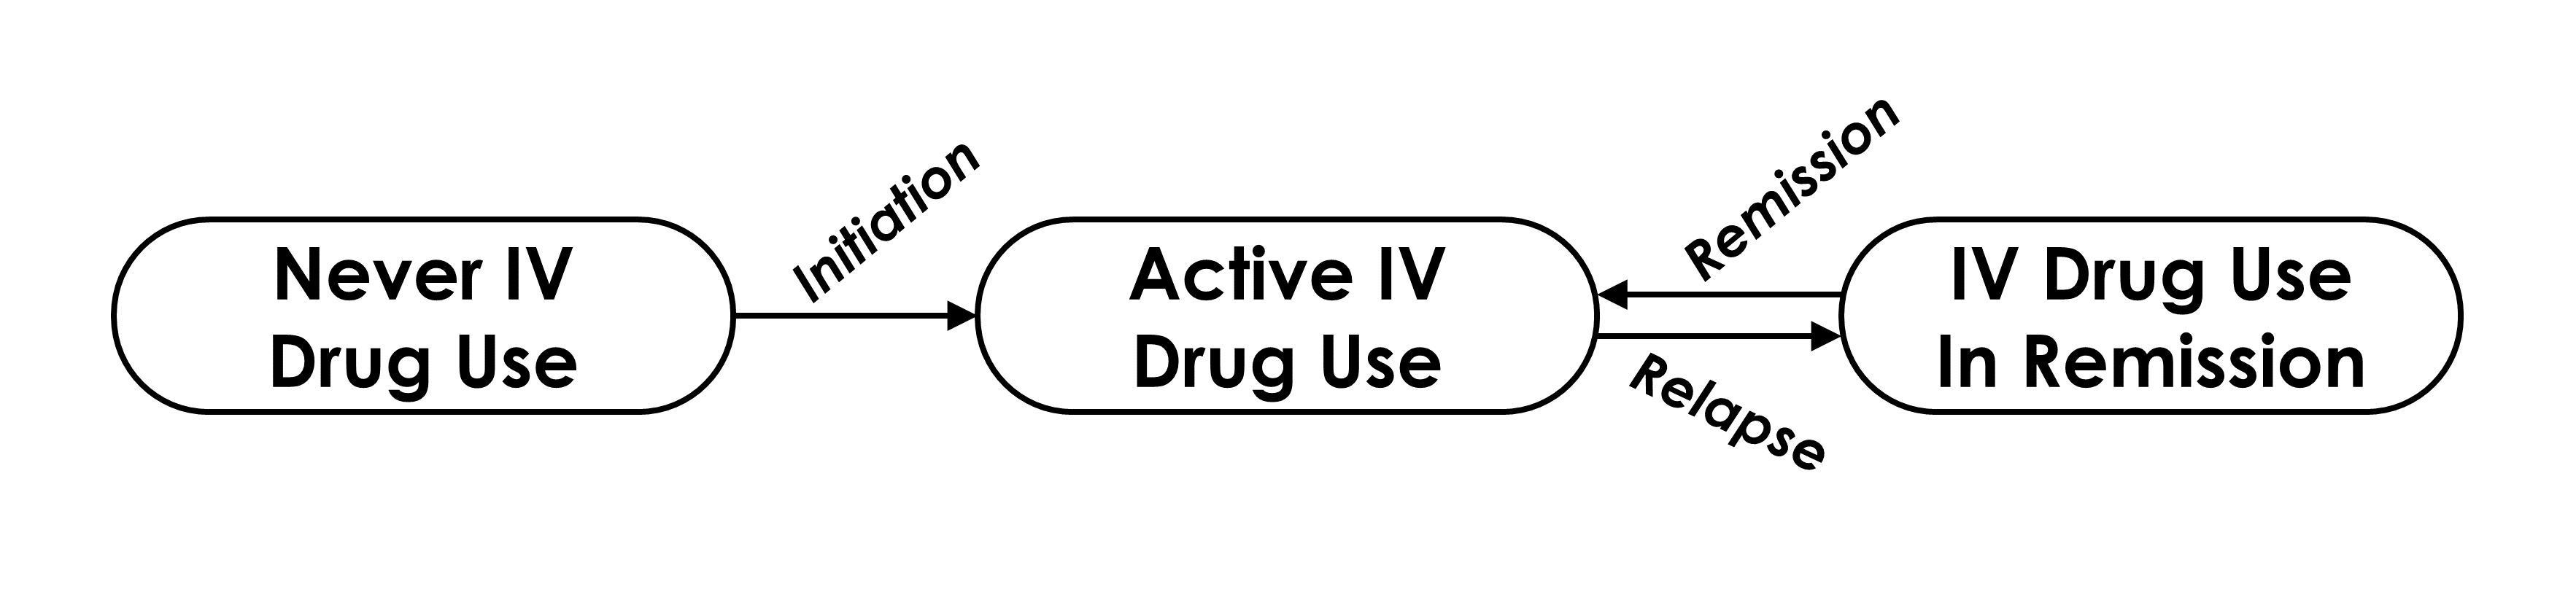
\includegraphics[width=0.75\textwidth]{base/images/idu_transitions}
	}
\end{figure}

\subsubsection{Time-Varying Parameters}

Many of the parameters in our differential equations are time-varying. We present the differential equations here using general formulations for time-varying parameters (e.g., $\theta(t)$ for mortality rate). In section \ref{functional_forms} - "\nameref{functional_forms}" - we present the specific functional forms we used to allow parameters to vary over time. 


\subsection{HIV Transmission}\label{transmission}

For shorthand, here we will replace $a,r,s,k$ by $i$ and $j$ to index strata of age $\times$ race $\times$ sex/sexual behavior $\times$ IV drug use, where there are $N=A\cdot R \cdot S \cdot K$ total strata ($i,j = 1, ..., N$)
\newline
\newline

The rate of new infections into stratum $i$ at time $t$ - denoted $\Delta_i(t)$ - is the sum of the rates of new infections by each of the $M$ modes of transmission:

\begin{equation}
\Delta_i(t) = \sum_{m=1}^M \Delta_{i,m}(t)
\end{equation}

where $\Delta_{i,m}(t)$ is the rate of new infections into stratum $i$ by transmission mode $m$ at time $t$, which is the sum over all strata $j$ of the rate of new infections into stratum $i$ from contact with stratum $j$ via mode $m$ of transmission:

\begin{equation}
\Delta_{i,m}(t) = \sum_{j=1}^N \Delta_{i,j,m}(t)
\end{equation}

where $\Delta_{i,j,m}(t)$ is the rate of new infections in stratum $i$ due to contact with those infected in stratum $j$ via a mode of transmission $m$ at time $t$. Broadly speaking, this is the product of:

\begin{itemize}
	\item The \textit{transmissibility} from stratum $j$ at time $t$, which is a function of the prevalence of unsuppressed PWH in the stratum.
	\item The proportion of stratum $i$'s partners who come from stratum $j$ (for transmission mode $m$) at time $t$, denoted $\Phi_{i,j,m}(t)$
	\item The rate  of transmission from stratum $j$ to stratum $i$ via mode $m$ at time $t$, denoted $\Gamma_{i,j,m}(t)$
	\item The \textit{susceptibility} of stratum $i$ to infection at time $t$ (in this work, this is a function of PrEP coverage within the stratum)
\end{itemize}

\begin{equation}
\Delta_{i,j,m} = transmissibility_{j,m}(t) \times \Phi_{i,j,m}(t) \times \Gamma_{i,j,m}(t) \times susceptibility_{i,m}(t)
\end{equation}

We describe $transmissibility$ and $susceptibility$ in further detail:

\subsubsection{Transmissibility}

The transmissibility of HIV from stratum $j$ via mode of transmission $m$ at time $t$ is a function of the prevalence of unsuppressed HIV in stratum $j$, allowing for PWH in the acute phase of HIV to transmit more and for those who are diagnosed to reduce transmission behaviors:

\begin{equation}
transmissibility_{j,m}(t) = \frac{\eta \cdot  IA_j(t) + IC_j(t) + \eta \cdot PA_j(t) + PC_j(t) + \eta \cdot \upsilon_j(t) \cdot DA_j(t) \cdot [1 - \rho_j(t)] + \upsilon_j(t) \cdot DC_j(t) \cdot [1 - \rho_j(t)]}{U_j(t) + IA_j(t) + IC_j(t) + PA_j(t) + PC_j(t) + DA_j(t) + DC_j(t)}
\end{equation}

where
\begin{itemize}
	\item $\eta$ is the ratio of transmissibility in the acute phase of HIV relative to the chronic phase
	\item $\rho_j(t)$ is the proportion of diagnosed PWH in stratum $j$ who are virally suppressed at time $t$
	\item $\upsilon_j(t)$ is the degree (relative rate) to which PWH who are aware of their diagnosis reduce their transmission behaviors, on average, relative to PWH who are unaware of their diagnosis
\end{itemize}

\subsubsection{Susceptibility}
\begin{equation}
susceptibility_{i,m}(t) = [1-\pi_i(t)] + \pi_i(t) \times \kappa_{i}
\end{equation}


\begin{itemize}
	\item $\pi_{i}(t)$ is the proportion uninfected individuals at risk for HIV in stratum $i$ at time $t$ who are enrolled in a PrEP program
	\item $\kappa_{i}$ is the relative risk of HIV infection for those on PrEP (relative to no PrEP) in stratum $i$
\end{itemize}


\subsection{Uninfected \big($U_{a,r,s,k}(t)$\big)}
The inflows into each stratum $a,r,s,k$ of uninfected are those entering the model at the youngest age bracket or aging into age stratum $a$ and those moving into IV drug use state $k$. The outflows are those who become infected with HIV, as well as those who die, age out of age stratum $a$, or move out of IV drug use state $k$.
\begin{align*}
	\frac{\partial U_{a,r,s,k}(t)}{\partial t} 
	&= \mathbbm{1}_{a=1} \times \lambda_{r} \times P_r(t) + \mathbbm{1}_{a>1} \times \alpha_{a-1,r,s,k}^U(t) \times U_{a-1,r,s,k}(t) \\
	&+ \mathbbm{1}_{k=active\_use} \times [\zeta_{a,r,s}(t) \times U_{a,r,s,never\_use}(t) + \xi_{a,r,s}(t) \times U_{a,r,s,prior\_use}(t)]\\
	&\qquad + \mathbbm{1}_{k=prior\_use} \times \psi_{a,r,s}(t) \times U_{a,r,s,active\_use}(t)\\
	&- \Delta_{a,r,s,k}(t) \\
	&- \theta^G_{a,r,s,k} \times U_{a,r,s,k}(t) - \mathbbm{1}_{k=active\_use} \times \theta^{IDU} \times U_{a,r,s,k}(t) \\
	&- \alpha_{a,r,s,k}^U(t) \times U_{a,r,s,k}(t) \\
	&- U_{a,r,s,k}(t) \times \big[\mathbbm{1}_{k=never\_use} \times \zeta_{a,r,s}(t) + \mathbbm{1}_{k=active\_use} \times \psi_{a,r,s}(t) + \mathbbm{1}_{k=prior\_use} \times \xi_{a,r,s}(t)\big]
\end{align*}

where
\begin{itemize}
	\item $\mathbbm{1}_{a=1}$ evaluates to 1 if $a$ is the first age bracket and 0 otherwise, and $\mathbbm{1}_{a>1}$ evaluates to 0 if $a$ is the first age bracket and 1 otherwise
	\item $\lambda_(t)$ denotes the birth rate for race $r$ at time $t$
	\item $P_r(t)$ is the total size of all strata where race = $r$ at time $t$. i.e.
		\begin{equation*}
			P_r(t) = \sum_{a,s,k} U_{a,r,s,k}(t) + IA_{a,r,s,k}(t) + IC_{a,r,s,k}(t) + PA_{a,r,s,k}(t) + PC_{a,r,s,k}(t) + DA_{a,r,s,k}(t) + DC_{a,r,s,k}(t)
		\end{equation*}
	\item $\alpha^U_{a-1,r,s,k}$ denotes the aging rate at time $t$ of uninfected individuals in the age stratum before $a$ - the average rate at which uninfected individuals move from age stratum $a-1$ to $a$
	\item $\mathbbm{1}_{k=active\_use}$ evaluates to 1 if $k$ denotes a compartment of active IV drug use and 0 otherwise, and $\mathbbm{1}_{k=prior\_use}$ evaluates to 1 if $k$ denotes a compartment of prior IV drug use
	\item $\zeta_{a,r,s}(t)$ denotes the rate of first-time initiation of IV drug use at time $t$ in stratum $a,r,s$
	\item $\xi_{a,r,s}(t)$ denotes the rate of relapse into IV drug use among prior users of IV drugs at time $t$ in stratum $a,r,s$
	\item $\psi_{a,r,s}(t)$ denotes the rate of remission of IV drug use among active users at time $t$ in stratum $a,r,s$
	\item $U_{a,r,s,never\_use}$, $U_{a,r,s,prior\_use}$, $U_{a,r,s,active\_use}$ denote the compartments with the same age, race, and sex/sexual behavior as $a,r,s,k$ but whose IV drug use stratum is "never use", "prior use", or "active use" respectively	
	\item $\Delta_{a,r,s,k}(t)$ denotes the number of new HIV infections in stratum $a,r,s,k$ at time $t$. This is detailed in Section \ref{transmission} on page \pageref{transmission}
	\item $\theta^G_{a,r,s,k}$ denotes the general mortality rate of individuals in stratum $a,r,s,k$
	\item  $\theta^{IDU}$ denotes the excess mortality rate due to active IV drug use
	\item $\alpha^U_{a,r,s,k}(t)$ denotes the aging rate at time $t$ for uninfected individuals in stratum $a,r,s,k$

\end{itemize}

\subsection{Undiagnosed, Acute HIV \big($IA_{a,r,s,k}(t)$\big)}

The inflows into each stratum $a,r,s,k$ of acute, undiagnosed HIV are the new infections among those who were not on PrEP, those aging into age stratum $a$, and those moving into IV drug use state $k$. The outflows are those who get diagnosed or progress to chronic HIV, as well as those who die (from HIV or other causes), age out of age stratum $a$, or move out of IV drug use state $k$.

\begin{align*}
\frac{\partial IA_{a,r,s,k}(t)}{\partial t} 
&= \Delta_{a,r,s,k}(t) \times [1-\mu_{a,r,s,k}(t)]\\
&+ \mathbbm{1}_{a>1} \times \alpha_{a-1,r,s,k}^H(t) \times IA_{a-1,r,s,k}(t) \\
&+ \mathbbm{1}_{k=active\_use} \times [\zeta_{a,r,s}(t) \times IA_{a,r,s,never\_use}(t) + \xi_{a,r,s}(t) \times IA_{a,r,s,prior\_use}(t)]\\
&\qquad + \mathbbm{1}_{k=prior\_use} \times \psi_{a,r,s}(t) \times IA_{a,r,s,active\_use}(t)\\
&- \beta_{a,r,s,k}(t) \times IA_{a,r,s,k}(t) \\
&- \tau \times IA_{a,r,s,k}(t) \\
&- \theta^{HIV}(t) \times IA_{a,r,s,k}(t)  
- \theta^G_{a,r,s,k} \times IA_{a,r,s,k}(t) 
- \mathbbm{1}_{k=active\_use} \times \theta^{IDU} \times IA_{a,r,s,k}(t) \\
&- \alpha_{a,r,s,k}^H(t) \times IA_{a,r,s,k}(t) \\
&- IA_{a,r,s,k}(t) \times \big[\mathbbm{1}_{k=never\_use} \times \zeta_{a,r,s}(t) + \mathbbm{1}_{k=active\_use} \times \psi_{a,r,s}(t) + \mathbbm{1}_{k=prior\_use} \times \xi_{a,r,s}(t)\big]
\end{align*}


where
\begin{itemize}
	\item $\mu_{a,r,s,k}(t)$ denotes the proportion of new infections in stratum $a,r,s,k$ at time $t$ that were among individuals on PrEP. 
	\begin{equation*}
		\mu_{a,r,s,k}(t) = \frac{\pi_{a,r,s,k}(t) \times \kappa_{a,r,s,k}}{[1-\pi_{a,r,s,k}(t)] + \pi_{a,r,s,k}(t) \times \kappa_{a,r,s,k}}
	\end{equation*} where $\pi_{a,r,s,k}(t)$ is the proportion uninfected individuals at risk for HIV in stratum $a,r,s,k$ at time $t$ who are enrolled in a PrEP program, and $\kappa_{a,r,s,k}$ is the relative risk of HIV infection for PrEP use in stratum $a,r,s,k$
	\item $\alpha_{a-1,r,s,k}^H(t)$ denotes the aging rate of HIV-positive individuals in the age stratum prior to $a$
	\item $\beta_{a,r,s,k}(t)$ is the rate of diagnosis of HIV for those in stratum $a,r,s,k$ at time $t$
	\item $\tau$ is the rate of progression from acute to chronic HIV
	\item $\theta^{HIV}(t)$ is the (time-varying) rate of excess mortality from unsuppressed HIV
	\item $\alpha^H_{a,r,s,k}(t)$ is the aging rate at time $t$ for PWH in stratum $a,r,s,k$
\end{itemize}

\subsection{Undiagnosed, Acute HIV, Enrolled in a PrEP Program \big($PA_{a,r,s,k}(t)$\big)}

The inflows into each stratum $a,r,s,k$ of acute, undiagnosed HIV among those enrolled in a PrEP program are the proportion of new infections among those who were on PrEP, those aging into age stratum $a$, and those moving into IV drug use state $k$. The outflows are those who get diagnosed or progress to chronic HIV, as well as those who die (from HIV or other causes), age out of age stratum $a$, or move out of IV drug use state $k$.

\begin{align*}
\frac{\partial PA_{a,r,s,k}(t)}{\partial t} 
&= \Delta_{a,r,s,k}(t) \times \mu_{a,r,s,k}(t)\\
&+ \mathbbm{1}_{a>1} \times \alpha_{a-1,r,s,k}^H(t) \times PA_{a-1,r,s,k}(t) \\
&+ \mathbbm{1}_{k=active\_use} \times [\zeta_{a,r,s}(t) \times PA_{a,r,s,never\_use}(t) + \xi_{a,r,s}(t) \times PA_{a,r,s,prior\_use}(t)]\\
&\qquad + \mathbbm{1}_{k=prior\_use} \times \psi_{a,r,s}(t) \times PA_{a,r,s,active\_use}(t)\\
&- \beta^{PrEP} \times PA_{a,r,s,k}(t) \\
&- \tau \times PA_{a,r,s,k}(t) \\
&- \theta^{HIV}(t) \times PA_{a,r,s,k}(t)  
- \theta^G_{a,r,s,k} \times PA_{a,r,s,k}(t) 
- \mathbbm{1}_{k=active\_use} \times \theta^{IDU} \times PA_{a,r,s,k}(t) \\
&- \alpha_{a,r,s,k}^H(t) \times PA_{a,r,s,k}(t) \\
&- PA_{a,r,s,k}(t) \times \big[\mathbbm{1}_{k=never\_use} \times \zeta_{a,r,s}(t) + \mathbbm{1}_{k=active\_use} \times \psi_{a,r,s}(t) + \mathbbm{1}_{k=prior\_use} \times \xi_{a,r,s}(t)\big]
\end{align*}

where
\begin{itemize}
	\item $\beta^{PrEP}$ is the rate of diagnosis of HIV among those enrolled in a PrEP program
\end{itemize}

\subsection{Diagnosed, Acute HIV \big($DA_{a,r,s,k}(t)$\big)}

The inflows into each stratum $a,r,s,k$ of acute, diagnosed HIV are new HIV diagnoses among those with undiagnosed, acute HIV (those enrolled in a PrEP program and not), those aging into age stratum $a$, and those moving into IV drug use state $k$. The outflows are those who progress to chronic HIV, as well as those who die (from unsuppressed HIV or other causes), age out of age stratum $a$, or move out of IV drug use state $k$.

\begin{align*}
\frac{\partial DA_{a,r,s,k}(t)}{\partial t} 
&= \beta_{a,r,s,k}(t) \times IA_{a,r,s,k}(t) + \beta^{PrEP} \times PA_{a,r,s,k}(t) \\
&+ \mathbbm{1}_{a>1} \times \alpha_{a-1,r,s,k}^H(t) \times DA_{a-1,r,s,k}(t) \\
&+ \mathbbm{1}_{k=active\_use} \times [\zeta_{a,r,s}(t) \times DA_{a,r,s,never\_use}(t) + \xi_{a,r,s}(t) \times DA_{a,r,s,prior\_use}(t)]\\
&\qquad + \mathbbm{1}_{k=prior\_use} \times \psi_{a,r,s}(t) \times DA_{a,r,s,active\_use}(t)\\
&- \beta_{a,r,s,k}(t) \times DA_{a,r,s,k}(t) \\
&- \tau \times DA_{a,r,s,k}(t) \\
&- \theta^{HIV}(t) \times DA_{a,r,s,k}(t) \times [1-\rho_{a,r,s,k}(t)]
- \theta^G_{a,r,s,k} \times DA_{a,r,s,k}(t) 
- \mathbbm{1}_{k=active\_use} \times \theta^{IDU} \times DA_{a,r,s,k}(t) \\
&- \alpha_{a,r,s,k}^H(t) \times DA_{a,r,s,k}(t) \\
&- DA_{a,r,s,k}(t) \times \big[\mathbbm{1}_{k=never\_use} \times \zeta_{a,r,s}(t) + \mathbbm{1}_{k=active\_use} \times \psi_{a,r,s}(t) + \mathbbm{1}_{k=prior\_use} \times \xi_{a,r,s}(t)\big]
\end{align*}

where
\begin{itemize}
	\item $\rho_{a,r,s,k}(t)$ is the proportion of those with diagnosed HIV in stratum $a,r,s,k$ who are virally suppressed at time $t$.
\end{itemize}

\subsection{Undiagnosed, Chronic HIV \big($IC_{a,r,s,k}(t)$\big)}

The inflows into each stratum $a,r,s,k$ of chronic, undiagnosed HIV are those who progress from acute to chronic HIV, those aging into age stratum $a$, and those moving into IV drug use state $k$. The outflows are those who get diagnosed, as well as those who die (from HIV or other causes), age out of age stratum $a$, or move out of IV drug use state $k$.

\begin{align*}
\frac{\partial IC_{a,r,s,k}(t)}{\partial t} 
&= \tau \times IA_{a,r,s,k}(t) \\
&+ \mathbbm{1}_{a>1} \times \alpha_{a-1,r,s,k}^H(t) \times IC_{a-1,r,s,k}(t) \\
&+ \mathbbm{1}_{k=active\_use} \times [\zeta_{a,r,s}(t) \times IC_{a,r,s,never\_use}(t) + \xi_{a,r,s}(t) \times IC_{a,r,s,prior\_use}(t)]\\
&\qquad + \mathbbm{1}_{k=prior\_use} \times \psi_{a,r,s}(t) \times IC_{a,r,s,active\_use}(t)\\
&- \beta_{a,r,s,k}(t) \times IC_{a,r,s,k}(t) \\
&- \theta^{HIV}(t) \times IC_{a,r,s,k}(t)  
- \theta^G_{a,r,s,k} \times IC_{a,r,s,k}(t) 
- \mathbbm{1}_{k=active\_use} \times \theta^{IDU} \times IC_{a,r,s,k}(t) \\
&- \alpha_{a,r,s,k}^H(t) \times IC_{a,r,s,k}(t) \\
&- IC_{a,r,s,k}(t) \times \big[\mathbbm{1}_{k=never\_use} \times \zeta_{a,r,s}(t) + \mathbbm{1}_{k=active\_use} \times \psi_{a,r,s}(t) + \mathbbm{1}_{k=prior\_use} \times \xi_{a,r,s}(t)\big]
\end{align*}

\subsection{Undiagnosed, Chronic HIV, Enrolled in a PrEP Program \big($PC_{a,r,s,k}(t)$\big)}

The inflows into each stratum $a,r,s,k$ of chronic, undiagnosed HIV among those enrolled in a PrEP program are those who progress from acute to chronic HIV, those aging into age stratum $a$, and those moving into IV drug use state $k$. The outflows are those who get diagnosed, as well as those who die (from HIV or other causes), age out of age stratum $a$, or move out of IV drug use state $k$.
\begin{align*}
\frac{\partial PC_{a,r,s,k}(t)}{\partial t} 
&= \tau \times PA_{a,r,s,k}(t) \\
&+ \mathbbm{1}_{a>1} \times \alpha_{a-1,r,s,k}^H(t) \times PC_{a-1,r,s,k}(t) \\
&+ \mathbbm{1}_{k=active\_use} \times [\zeta_{a,r,s}(t) \times PC_{a,r,s,never\_use}(t) + \xi_{a,r,s}(t) \times PC_{a,r,s,prior\_use}(t)]\\
&\qquad + \mathbbm{1}_{k=prior\_use} \times \psi_{a,r,s}(t) \times PC_{a,r,s,active\_use}(t)\\
&- \beta^{PrEP} \times PC_{a,r,s,k}(t) \\
&- \theta^{HIV}(t) \times PC_{a,r,s,k}(t)  
- \theta^G_{a,r,s,k} \times PC_{a,r,s,k}(t) 
- \mathbbm{1}_{k=active\_use} \times \theta^{IDU} \times PC_{a,r,s,k}(t) \\
&- \alpha_{a,r,s,k}^H(t) \times PC_{a,r,s,k}(t) \\
&- PC_{a,r,s,k}(t) \times \big[\mathbbm{1}_{k=never\_use} \times \zeta_{a,r,s}(t) + \mathbbm{1}_{k=active\_use} \times \psi_{a,r,s}(t) + \mathbbm{1}_{k=prior\_use} \times \xi_{a,r,s}(t)\big]
\end{align*}

\subsection{Diagnosed, Chronic HIV \big($DC_{a,r,s,k}(t)$\big)}

The inflows into each stratum $a,r,s,k$ of chronic, diagnosed HIV are new HIV diagnoses among those with undiagnosed, chronic HIV (those enrolled in a PrEP program and not), those who progress from acute to chronic HIV, those aging into age stratum $a$, and those moving into IV drug use state $k$. The outflows are those who die (from unsuppressed HIV or other causes), age out of age stratum $a$, or move out of IV drug use state $k$.

\begin{align*}
\frac{\partial DC_{a,r,s,k}(t)}{\partial t} 
&= \beta_{a,r,s,k}(t) \times IC_{a,r,s,k}(t) + \beta^{PrEP} \times PC_{a,r,s,k}(t) \\
&+ \tau \times DA_{a,r,s,k}(t) \\
&+ \mathbbm{1}_{a>1} \times \alpha_{a-1,r,s,k}^H(t) \times DC_{a-1,r,s,k}(t) \\
&+ \mathbbm{1}_{k=active\_use} \times [\zeta_{a,r,s}(t) \times DC_{a,r,s,never\_use}(t) + \xi_{a,r,s}(t) \times DC_{a,r,s,prior\_use}(t)]\\
&\qquad + \mathbbm{1}_{k=prior\_use} \times \psi_{a,r,s}(t) \times DC_{a,r,s,active\_use}(t)\\
&- \beta_{a,r,s,k}(t) \times DC_{a,r,s,k}(t) \\
&- \theta^{HIV}(t) \times DC_{a,r,s,k}(t) \times [1-\rho_{a,r,s,k}(t)]
- \theta^G_{a,r,s,k} \times DC_{a,r,s,k}(t) 
- \mathbbm{1}_{k=active\_use} \times \theta^{IDU} \times DC_{a,r,s,k}(t) \\
&- \alpha_{a,r,s,k}^H(t) \times DC_{a,r,s,k}(t) \\
&- DC_{a,r,s,k}(t) \times \big[\mathbbm{1}_{k=never\_use} \times \zeta_{a,r,s}(t) + \mathbbm{1}_{k=active\_use} \times \psi_{a,r,s}(t) + \mathbbm{1}_{k=prior\_use} \times \xi_{a,r,s}(t)\big]
\end{align*}


%---------------------------------%
%-- CALIBRATION METHOD --%
%---------------------------------%

\section{Running And Calibrating the Model}

\subsection{Initializing and Running the Model}

We initialize the model with population sizes from 2007, and seed three HIV cases, one to each race, in the stratum of MSM aged 35-44yo.

We let the model start running at 1970 with this initial state, and run forward to 2007. From 1970 to 2007, we keep the sizes of each stratum of age $\times$ race $\times$ sex/sexual behavior constant; the prevalence of HIV and IV drug use states can vary within these strata. (Fixing strata sizes allowed us to avoid having to replicate birth patterns prior to the 2010-2030 time period).

We continue running the model from 2007 to 2030, without the requirement that strata sizes remain constant.


\subsection{Calibration Method}
To fit our 131 sampled parameters in each MSA, we use Adaptive Metropolis Sampling, a Markov-chain Monte-Carlo technique first described by Haario et. al.\cite{haario2001}. We use a variation of algorithm 5 ("componentwise" sampling) in Andrieu et. al \cite{andrieu2008}, in which we sample blocks of 1 to 6 parameters at a time in a "blockwise" fashion.

For each iteration of the MCMC, we: 
\begin{enumerate}
	\item Sample the new parameters for the block
	\item Run a simulation using the parameters (the new values for parameters in the block, and prior values for parameters not in the block)
	\item Compute the likelihood (and prior for the parameters) and accept or reject
\end{enumerate}

\subsubsection{Finding Initial Parameter Values} \label{init_params}
For each location, we developed a set of starting parameter values by manually calibrating transmission rates and age susceptibilities so that the marginal reported diagnoses and prevalence by age, by race, and by risk factor visually approximated the calibration targets. All other parameter values were left at their "best guess" values (the median for parameters following a Log-normal prior).

Using these starting values, we ran an exploratory, single-chain Adaptive Metropolis Sampling Process for 20,000 iterations with a target acceptance rate of 0.10. We discarded the first 10,000 parameter sets and thinned the remainder to every 20th set, yielding 500 parameter sets. For each parameter value, we calculated a mean and standard deviation on the log scale across the 500 values, as well as correlations with all other parameters. We used the resulting Log-Multivariate-Normal distribution to sample initial parameters for the MCMC runs described below.


\subsubsection{Likelihood and Priors}

In our deterministic, compartmental model, there is a one-to-one correlation between parameters and simulations. The likelihood function can only be computed on a simulation once it has run. Our log-likelihood is actually the sum of ten independent sub-likelihoods, detailed in Section \ref{likelihood}.

The prior distributions for parameters are mostly Log-Normal distributions (a few are Logit-Normal or Uniform), as detailed in Table \ref{params_tab}.

\subsubsection{MCMC Sampling}

For each location, we ran four chains, sampling starting parameter values for each chain from the Log-Multivariate-Normal distribution described above in section \ref{init_params}. For each chain, we ran 50,000 burn-in iterations followed by 50,000 sampling iterations. We thinned to every 200th iteration, leaving us with a set of 1,000 simulations. We used a target acceptance rate of 0.234.

We assessed for convergence using the split-$\hat{r}$ described in Gelman,\cite{gelman2014} as well as visual inspection of trace plots for important or poorly mixing parameters.


%---------------------------------%
%-- LIKELIHOOD --%
%---------------------------------%


\section{The Likelihood} \label{likelihood}

Our likelihood decomposes into 10 independent likelihoods for each of the 10 calibration targets: new diagnoses, prevalence, HIV mortality, proportion of PWH aware of their diagnosis, proportion of PWH virally suppressed, number of at-risk individuals receiving prescriptions for emtricitabine/tenofovir, probability of receiving an HIV test, prevalence of injection drug use, historical AIDS mortality (prior to 2002), and historical reported diagnoses (1998-2002).

\subsection{Calibrating Model Rates to Observed Data: Binomial Likelihood}\label{binomial_likelihood}
In general, for each of our outcome targets, we will use some variation of a binomial likelihood that maps the probability of an outcome in stratum $i$ in a simulation to the number of events in reported data.

\begin{equation}
	y_{i,t} \sim Binomial(n_t, p_{i,t})
\end{equation}

where
\begin{itemize}
	\item $y_{i,t}$ is the reported outcome in subgroup $i$ at time $t$
	\item $n_t$ is the total population size at time $t$
	\item $p_{i,t}$ is the simulated outcomes in subgroup $i$ at time $t$ divided by the simulated total population size at time $t$
\end{itemize}

Note that we scale our outcome probabilities - even for a subgroup - relative to the total population. For example, if we were calibrating to the number of reported diagnoses in MSM in 2015, $p_{i,t}$ would be the simulated number of new infections among MSM in 2015 divided by the \textit{total} simulated population in 2015. Similarly, the $n_t$ used in our likelihood represents the \textit{total} population, even when calibrating a subgroup.

Formulating the likelihood in this way allows us to avoid conditioning on subgroup numbers that are not known or known imperfectly. For example, the true number of MSM is not recorded by the US census. While estimates are available, they are imprecise and not stratified by race.

In actuality, we use the Normal approximation to the binomial, which is computationally more efficient and allows us to formulate multivariate likelihoods easily:
\begin{equation}
	y_{i,t} \sim Normal\Big(n_t \cdot p_{i,t}, n_t \cdot p_{i,t} \cdot (1-p_{i,t}) \Big)
\end{equation}

\subsection{Mapping Outcomes in Stratified Compartments to Reported Marginal Observations}\label{likelihood_mapping}

Our model produces estimates of each outcome in 135 strata per year of age (5 brackets), race (Black, Hispanic, Other), sex/sexual behavior (MSM, heterosexual male, female), and IV drug use (never use, active use, prior use). Calibration targets are rarely reported as fully stratified. To calibrate to marginal data, we use a multivariate likelihood which uses matrix multiplication to aggregate strata into marginal subgroups.

To illustrate, we use a simplified example in which a model partitions the population four strata of age (young vs. old) and sex (male vs. female), but calibrates to marginal outcomes at time $t$: $y_{young,t}$, $y_{old,t}$, $y_{male,t}$, $y_{female,t}$.

We presume that:
\begin{align*}
	y_{young,t} &= y_{young,male,t} + y_{young,female,t}\\
	y_{old,t} &= y_{old,male,t} + y_{old,female,t}\\
	y_{male,t} &= y_{young,male,t} + y_{old,male,t}\\
	y_{female,t} &= y_{young,female,t} + y_{old,female,t}\\
\end{align*}
$y_{young,male,t}$, $y_{young,female,t}$, $y_{old,male,t}$, $y_{old,female,t}$ are not actually reported. However, we formulate the likelihood we would use if they were, using an independent, binomial likelihood for each of the four stratified outcomes:

\begin{align*}
	y_{young,male,t} &\sim Binomial(n_t, p_{young,male,t}) \\
	y_{young,female,t} &\sim Binomial(n_t, p_{young,female,t}) \\
	y_{old,male,t} &\sim Binomial(n_t, p_{old,male,t}) \\
	y_{old,female,t} &\sim Binomial(n_t, p_{old,female,t}) \\
\end{align*}

For computational efficiency and to facilitate multivariate formulation, we use the normal approximation to the binomial:

\begin{align*}
	y_{young,male,t} &\sim Normal\big(n_t \times p_{young,male,t}, n_t \times p_{young,male,t} \times (1-p_{young,male,t})\big) \\
	y_{young,female,t} &\sim Normal\big(n_t \times p_{young,female,t}, n_t \times p_{young,female,t} \times (1-p_{young,female,t})\big) \\
	y_{old,male,t} &\sim Normal\big(n_t \times p_{old,male,t}, n_t \times p_{old,male,t} \times (1-p_{old,male,t})\big) \\
	y_{old,female,t} &\sim Normal\big(n_t \times p_{old,female,t}, n_t \times p_{old,female,t} \times (1-p_{old,female,t})\big) \\
\end{align*}

We write this as a multivariate normal distribution with a mean vector corresponding to the four individual means and a diagonal variance-covariance matrix whose diagonal elements are the four individual variances:

\begin{equation}
	\bm{y_t^\prime} = 
	\begin{bmatrix}
	y_{young,male,t} \\ y_{young,female,t} \\ y_{old,male,t} \\ y_{old,female,t}
	\end{bmatrix} \sim Multivariate\text{-}Normal(\bm{\mu_t}, \bm{\Sigma_t})
\end{equation}

Next, we formulate a matrix, $\bm{M}$, that maps from the unobserved, stratified outcomes to the marginal outcomes which we do observe:

\begin{equation}
	\bm{y_t} = \begin{bmatrix}
		y_{young,t} \\ y_{old,t} \\ y_{male,t} \\ y_{female,t}
	\end{bmatrix} =
	\begin{bmatrix}
	1 & 1 & 0 & 0 \\
	0 & 0 & 1 & 1 \\
	1 & 0 & 1 & 0 \\
	0 & 1 & 0 & 1 \\
	\end{bmatrix}
	\begin{bmatrix}
	y_{young,male,t} \\ y_{young,female,t} \\ y_{old,male,t} \\ y_{old,female,t}
	\end{bmatrix} =
	\bm{M_t} \begin{bmatrix}
	y_{young,male,t} \\ y_{young,female,t} \\ y_{old,male,t} \\ y_{old,female,t}
	\end{bmatrix} =
	\bm{M_t} \bm{y_t^\prime}
\end{equation}

Using this matrix, we can map the likelihood over the unobserved, stratified outcomes to a likelihood over the observed, marginal outcomes:
\begin{equation}
	\bm{y_t} \sim Multivariate\text{-}Normal\big(\bm{M_t \mu_t}, \bm{M \Sigma_t M_t^T}\big)
\end{equation}

This formulation preserves the correlations induced by calibrating to marginal outcomes. For example, if a simulation over-estimated the young, male stratum, we would expect the overestimation of both the total young and overestimation of the total male to be related.

We can extend this approach to formulate a matrix $\bm{M}$ that maps our 135 strata to any set of marginal outcomes. We can map to two-level marginals (e.g., new diagnoses reported by sex and age bracket).

We can also extend this approach across multiple years by assuming that the errors in any one year are independent of other years:

\begin{equation}
	\bm{y} = 
	\begin{bmatrix}
		\bm{y_{t1}} \\
		\bm{y_{t2}} \\
		\vdots \\
		\bm{y_{tT}}
	\end{bmatrix}
	\sim Multivariate\text{-}Normal\big(\bm{M} \bm{\mu}, \bm{M} \bm{\Sigma} \bm{M}^T\big) \label{eq_mapping}
\end{equation}

where
\begin{itemize}
	\item $T$ is the number of years we include
	\item $\bm{\mu} = \begin{bmatrix}
		\bm{\mu_{t1}} \\
		\bm{\mu_{t2}} \\
		\vdots \\
		\bm{\mu_{tT}}
		\end{bmatrix}$
	\item $\bm{M} = \begin{bmatrix}
		\bm{M_{t1}} & \bm{0} & \dots & \bm{0} \\
		\bm{0} & \bm{M_{t2}} & \dots & \bm{0} \\
		\vdots & \vdots & \ddots & \vdots \\
		\bm{0} & \bm{0} & \dots & \bm{M_{tT}}
		\end{bmatrix}$
	\item $\bm{\Sigma} = \begin{bmatrix}
		\bm{\Sigma_{t1}} & \bm{0} & \dots & \bm{0} \\
		\bm{0} & \bm{\Sigma_{t2}} & \dots & \bm{0} \\
		\vdots & \vdots & \ddots & \vdots \\
		\bm{0} & \bm{0} & \dots & \bm{\Sigma_{tT}}
		\end{bmatrix}$
\end{itemize}	



\subsection{Incorporating Measurement Error}\label{measurement_error}

The formulation described in Section \ref{likelihood_mapping} above captures error that stems from the degree to which model simulations depart from reported outcomes. However, we also consider that reported outcomes are imperfect measures of a "true" outcome, and adjust our likelihoods accordingly.
For this formulation, we introduce $y^*_{i,t}$ - the true (unobserved) outcome for subgroup $i$ at time $t$, and use it to decomponse the relationship between $y_{i,t}$ - the reported outcome - and simulated outcomes.

For every subgroup $i$ and time $t$, we write:

\begin{equation}
	y_{i,t} = y^*_{i,t} + Bias_{i,t} + \epsilon_{i,t} \label{eq_reported_to_truth}
\end{equation}

\begin{itemize}
	\item $y_{i,t}$ is the reported (measured) outcome for subgroup $i$ at time $t$ to which we calibrate
	\item $y^*_{i,t}$ is the true (unobserved) outcome 
	\item $Bias_{i,t}$ represents the bias.	We set this term to zero for most reported outcomes. However, some outcomes are expected to differ systematically from the truth. For example, with respect to HIV mortality, it is known that a small proportion of deaths in PWH are not reported to the National Death Index \cite{hanna2009,trepka2011}.
	\item $\epsilon_{i,t}$ The measurement error for outcome $y_{i,t}$
\end{itemize}

We can vectorize Equation \ref{eq_reported_to_truth}
\begin{equation}
	\bm{y} = \bm{y^*} + \bm{Bias} + \bm{\epsilon}
\end{equation}

We let
\begin{equation}
	\bm{Bias} \sim Multivariate\textit{-}Normal\Big(\bm{B}, \bm{\Sigma_B}\Big) \label{eq_bias}
\end{equation}

\begin{equation}
	\bm{\epsilon} \sim Multivariate\textit{-}Normal\Big(\bm{0}, \bm{\Sigma_\epsilon}\Big) \label{eq_epsilon}
\end{equation}

And we replace $\bm{y}$ in Equation \ref{eq_mapping} with $\bm{y^*}$:
\begin{equation}
	\bm{y^*} \sim Multivariate\text{-}Normal\big(\bm{M} \bm{\mu}, \bm{M} \bm{\Sigma} \bm{M}^T\big) \label{eq_mapping_ystar}
\end{equation}

We can combine Equations \ref{eq_bias}, \ref{eq_epsilon}, and \ref{eq_mapping_ystar} to yield a likelihood that incorporates different sources of error: the degree to which the model deviate from the truth, measurement error of reported outcomes, and bias.

\begin{equation}
	\bm{y} \sim Multivariate\textit{-}Normal\Big(\bm{M} \bm{\mu} + \bm{B},
		\bm{M} \bm{\Sigma} \bm{M}^T + \bm{\Sigma_B} + \bm{\Sigma_\epsilon}\Big)
\end{equation}

\subsubsection{Correlated Measurement Errors}\label{correlated_measurement_error}

We also allow for measurement errors and bias to be correlated over time. For example, if estimated prevalent HIV cases among MSM are overestimated in 2015, they are likely to be overestimated in 2016 and 2017 when using the same methods.\cite{fojo2017} To represent these correlations, we decompose $\bm{\Sigma_\epsilon}$ and $\bm{\Sigma_B}$ into a vector of standard deviations, $\bm{\sigma}$ and a correlation matrix, $\bm{\Lambda}$:


\begin{align}
	\bm{\Sigma_\epsilon} &= \bm{\sigma_\epsilon} \bm{\Lambda_\epsilon} \bm{\sigma_\epsilon^T}\\
	\bm{\Sigma_B} &= \bm{\sigma_B} \bm{\Lambda_B} \bm{\sigma_B^T}
\end{align}

In most cases, we give $\bm{\Lambda_\epsilon}$ and $\bm{\Lambda_B}$ a compound symmetry (AKA exchangeable) structure:
\begin{equation}
	\Lambda_{ij} = \begin{cases}
		1 & \text{if } i=j \\
		\rho & \text{if } i \neq j
	\end{cases}
\end{equation}

In general we formulate the standard deviations, $\sigma$ using a coefficient of variance: $\sigma_{i,t} = y_{i,t} \times cv_{i,t}$. We estimate the coefficients of variance and correlation parameters based off of reported data where possible.

%-- Reported Diagnoses --%
\subsection{Reported Diagnoses 2008-2018}

\subsubsection{Calibration Targets}
We calibrate to reported diagnoses from 2008-2018 as reported by the CDC in HIV Atlas\cite{hivatlas} and Metropolitan Statistical Area Reports\cite{msa2010,msa2011,msa2013,msa2014,msa2015,msa2016,cdc24.2}. We fit to total as well as stratified data when available (the years 2010,2011, and 2013-2017):
\begin{itemize}
	\item Total diagnoses for all years 2008-2018
	\item Stratified by age $\times$ sex for 2010, 2011, and 2013-2017
	\item Stratified by race $\times$ sex for 2010, 2011, and 2013-2017
	\item Stratified by risk factor $\times$ sex for 2010, 2011, and 2013-2017
	\item Stratified by race $\times$ risk factor for 2010, 2011, and 2013-2017
\end{itemize}

When the sum of stratified diagnoses from MSA reports did not equal the reported total diagnoses from HIV Atlas, we scaled the stratified diagnoses such that they summed to the total, but maintained the relative proportions of the MSA report.

\subsubsection{Measurement Error}

Because HIV Atlas estimates differed from those in the MSA reports, we were able to estimate the standard deviations of measurement errors by treating the HIV Atlas estimates as truth and the MSA reports as a measured quantity. We formulated the standard deviation as a coefficient of variance multiplied by the estimate, and derived a frequentist maximum likelihood estimate of 0.065 for the coefficient of variance.

Because there was a change in the method of reporting from 2014 to 2015, we assumed that 2008-2014 errors were strongly correlated with a correlation of 0.65, as were 2015-2018 errors, but that errors from the years 2008-2014 had a weaker correlation of 0.25 with errors from 2015-2018.

\subsubsection{Likelihood Formulation}

Using the error terms above, we formulated a multivariate normal likelihood based off of a binomial (Section \ref{binomial_likelihood}) with a mapping to account for correlations between overlapping strata (Section \ref{likelihood_mapping}) and correlated measurement errors (Section \ref{correlated_measurement_error}) using the error terms described above.

\subsubsection{Variance Inflation}
To improve parameter mixing in the MCMC, we inflate the variances for this likelihood by a factor of 4.


%-- Prevalence --%
\subsection{Estimated Prevalence 2008-2018}

\subsubsection{Calibration Targets}
We calibrate to the estimated prevalence (of those aware of their diagnosis) from 2008-2018 as reported by the CDC in HIV Atlas\cite{hivatlas} and Metropolitan Statistical Area Reports\cite{msa2010,msa2011,msa2013,msa2014,msa2015,msa2016,cdc24.2}. We fit to total as well as stratified data when available (the years 2009, 2010, and 2012-2016):
\begin{itemize}
	\item Total diagnoses for all years 2008-2018
	\item Stratified by age $\times$ sex for 2009, 2010, and 2012-2016
	\item Stratified by race $\times$ sex for 2009, 2010, and 2012-2016
	\item Stratified by risk factor $\times$ sex for 2009, 2010, and 2012-2016
	\item Stratified by race $\times$ risk factor for 2009, 2010, and 2012-2016
\end{itemize}

When the sum of stratified prevalence from MSA reports did not equal the reported total prevalence from HIV Atlas, we scaled the stratified prevalences such that they summed to the total, but maintained the relative proportions of the MSA report.

\subsubsection{Measurement Error} \label{prevalence_measurement_error}

As with reported diagnoses, we were able to estimate the standard deviations of measurement errors by treating the HIV Atlas estimates as truth and the MSA reports as a measured quantity. We formulated the standard deviation as a coefficient of variance multiplied by the estimate, and derived a frequentist maximum likelihood estimate of 0.09 for the coefficient of variance.

Because there was a change in the method of reporting from 2014 to 2015, we assumed that 2008-2013 errors were strongly correlated with a correlation of 0.65, as were 2014-2018 errors, but that errors from the years 2008-2013 had a weaker correlation of 0.25 with errors from 2014-2018.

\subsubsection{Likelihood Formulation}

As with reported diagnoses, we formulated a multivariate normal likelihood based off of a binomial (Section \ref{binomial_likelihood}) with a mapping to account for correlations between overlapping strata (Section \ref{likelihood_mapping}) and correlated measurement errors (Section \ref{correlated_measurement_error}) using the error terms described above.

\subsubsection{Variance Inflation}
To improve parameter mixing in the MCMC and to prevent the likelihood for prevalence from dominating the likelihood for reported diagnoses (prevalence has a much larger $p$ than reported diagnoses, so a much smaller binomial variance), we inflate the variances for this likelihood by a factor that is equal to the square-root of the average total prevalence from 2010-2018 divided by the square-root of the average number of reported diagnoses from 2010-2018.

%-- Mortality --%
\subsection{Mortality in PWH 2009-2016}

\subsubsection{Calibration Targets}
We calibrate to the mortality among PWH aware of their diagnosis in 2009, 2010, and 2012-2016 as reported by the CDC in Metropolitan Statistical Area Reports \cite{msa2010,msa2011,msa2013,msa2014,msa2015,msa2016,cdc24.2}. We fit to total mortality as well as mortality stratified by sex.

\subsubsection{Measurement Error}

We took the standard deviation to be a product of the coefficient of variance and the mortality estimate. We used the same coefficient of variance calculated for prevalence (0.09), as well as correlation coefficients (0.65 for 2009-2013 errors with 2009-2013 errors, 0.65 for 2014-2016 errors with 2014-2016 errors, and 0.25 for 2009-2013 errors with 2014-2016 errors).

\subsubsection{Bias}

Because a small proportion of deaths in PWH are not captured by the National Death Index \cite{hanna2009,trepka2011}, we presumed that mortality was biased down by 2.6\% with a standard deviation of 1.3\%.\cite{hanna2009,trepka2011}

\subsubsection{Likelihood Formulation}

We formulate a multivariate normal likelihood analagous to the likelihood for reported diagnoses and mortality, with the addition of the bias term as outlined in Section \ref{measurement_error}.

\subsubsection{Variance Inflation}
To improve parameter mixing in the MCMC, we inflate the variances for this likelihood by a factor of 2.



%-- Awareness of Diagnosis --%
\subsection{Awareness of Diagnosis Among PWH 2010-2018}\label{likelihood_awareness}

\subsubsection{Calibration Targets}
We calibrate to the proportion of PWH who are aware of their disease. For five MSAs (Houston-The Woodlands-Sugar Land, TX; Los Angeles-Long Beach-Anaheim, CA; Memphis, TN-MS-AR; New York-Newark-Jersey City, NY-NJ-PA; Seattle-Tacoma-Bellevue, WA) estimates of the proportion aware for at least 3 years from 2010-2018 were publicly available from local public health websites. For the remaining 27 MSAs, we used the state-level estimates of proportion aware of their diagnoses available through HIV Atlas \cite{hivatlas}. For MSAs that spanned multiple states, we calibrated to the weighted average of the proportion aware, where weights were the population within in the MSA that falls into each state from 2010-2018.

\subsubsection{Formulation of Binomial Likelihood Component}

For each year $t$, we postulated that:
\begin{equation}
	y_t \sim Binomial(\frac{y_t}{\pi_t}, p_t)
\end{equation}

where:
\begin{itemize}
	\item $y_t$ is the prevalence of PWH aware of their diagnosis in year $t$ as reported by the CDC
	\item $\pi_t$ represents our calibration target, the proportion of PWH aware of their diagnosis in year $t$ as reported by the CDC or local health department
	\item $\frac{y_t}{\pi_t}$ is the estimated number of all PWH (both those aware and unaware of their diagnosis) in year $t$
	\item $p_t$ is the simulated proportion of PWH aware of their diagnosis in year $t$
\end{itemize}

In order to generalize to a multivariate likelihood, we used the normal approximation to the binomial:

\begin{equation}
	y_t \sim Normal\Big(\frac{y_t}{\pi_t} \cdot p_t, \frac{x_t}{\pi_t} \cdot p_t \cdot (1 - p_t)\Big)
\end{equation}

\subsubsection{Measurement Error}

We included a measurement error as described in section \ref{correlated_measurement_error}. We assumed that the reported proportion of PWH aware of their diagnosis had a standard deviation of 0.005 when based on county- or MSA-level data data, and a standard deviation of 0.015 when based on state-level data.

We furthermore presumed that measurement errors were correlated across time, using a compound symmetry correlation structure with $\rho = 0.5$

\subsubsection{Likelihood Formulation}
We incorporated the Binomial component and measurement error into a multivariate normal likelihood as described in \ref{likelihood_mapping}.

\subsubsection{Variance Inflation}
To improve parameter mixing in the MCMC, we inflate the variances for this likelihood by a factor of 8.

%-- Viral Suppression --%
\subsection{Viral Suppression Among PWH 2010-2018}\label{likelihood_suppression}

The likelihood for suppression had two independent components: a multivariate-normal component targeting the reported proportion of PWH who were suppressed, and a Bernoulli component to weight whether suppression was increasing or decreasing.

\subsubsection{Calibration Targets}
We calibrated to the proportion of PWH who were suppressed, as reported on local health department websites, for all years between 2010 and 2018 where data were available. If multiple jurisdictions within an MSA reported proportions, we took the weighted average. If no data was available at the county- or MSA-level we used state-level proportions. A total proportion suppressed was available for all 32 MSAs; we also included estimates stratified by age, by race, by sex, and by HIV-acquisition risk factor if they were available.

\subsubsection{Binomial Likelihood Component}

We formulated a multivariate-normal approximation to a Binomial likelihood, similar to the one detailed in Section \ref{binomial_likelihood} with the exceptions that (1) the response was the CDC-reported prevalence of HIV multiplied by the reported proportion suppressed and (2) that the $n$ was the simulated prevalence of diagnosed HIV instead of the total population. We used the matrix mapping described in Section \ref{likelihood_mapping} to account for correlations in overlapping stratifications.

\subsubsection{Measurement Error}
We included a measurement error as described in section \ref{correlated_measurement_error}. We assumed that the reported proportion of PWH aware of their diagnosis had a standard deviation of 0.01 when based on county- or MSA-level data data, and a standard deviation of 0.03 when based on state-level data.

We furthermore presumed that measurement errors were correlated across time, using a compound symmetry correlation structure with $\rho = 0.5$

\subsubsection{Multivariate Normal Likelihood Formulation}
We incorporated the Binomial component and measurement error into a multivariate normal likelihood as described in \ref{likelihood_mapping}.

\subsubsection{Bernoulli Likelihood for Increasing vs. Decreasing Suppression}
In general, suppression is increasing or stable over time in most locations across most subgroups. In order to discourage solutions where one race or age subgroup had decreasing suppression over time but total suppression followed overall trends (which was possible in locations where stratified data on suppression were unavailable), we also included a Bernoulli likelihood. This likelihood specified that the probability that, for each stratum of age, race, sex, and IV drug use, the probability that simulated suppression had a decreasing slope on the logit scale was 0.05 (which we estimated from the average number of reported suppressed proportions that decreased from one year to the next in all locations and all stratifications for which we had data). ie:

\begin{equation}
	\prod_{a,r,s,k} 0.05^{\text{suppression in stratum } a,r,s,k \text{ is decreasing}} \times 0.95^{\text{suppression in stratum } a,r,s,k \text{ is not decreasing}}
\end{equation}




%-- PrEP --%
\subsection{Pharmacy Fills of Prescriptions for PrEP 2012-2018}\label{likelihood_prep}

\subsubsection{Calibration Targets}
We calibrated to the number of prescriptions for Emtricitabine/Tenofovir for use as PrEP from 2012 to 2018, as reported by AIDSVu \cite{aidsvu_prep}. We used both total numbers as well as numbers stratified by age and by sex (although, due to data suppression rules, stratified estimates were sometimes missing).

\subsubsection{Differences between Model Representation and Reported Data}
The concept of PrEP in our model differs from the data reported by AIDSVu in a number of ways, and our likelihood has to make adjustments for these discrepancies.

Our model simulations produce a proportion of at-risk individuals who are currently enrolled in a PrEP program (since most prescriptions for PrEP are written on a 3-month basis, we take this to correspond to a prescription in the past 3 months).

The AIDSVu data report the number of individuals who filled at least one prescription for emtricitabine/tenofovir in the past year, and who were not using it (as judged by a validated algorithm \cite{maccannell2015}) for treatment of HIV infection or viral hepatitis. Pharmacy records come from a commercial dataset that captures 83\% of prescriptions nationally. \cite{sullivan2018}

This introduces several discrepancies:
\begin{enumerate}
	\item Not all individuals who have a prescription for PrEP will be captured in the dataset
	\item Some individuals who take emtricitabine/tenofovir for indications other than PrEP (HIV treatment, viral hepatitis) will be incorrectly classified as taking it for PrEP
	\item Not all individuals who filled a PrEP prescription in the past year will have filled in the past 3 months (ie, have an "active" prescription)
\end{enumerate}

\subsubsection{Adjusting the Calibration Target to Account for Discrepancies}

We mapped our model output to the calibration target - the number of pharmacy fills for emtricitabine/tenofovir - using four adjustment factors, as follows:

\begin{equation}
	y^\prime_i = y_i \times \frac{\pi \cdot \phi \cdot \rho}{\theta}
\end{equation}

where:
\begin{itemize}
	\item $y_{i,t}$ Represents the reported number of pharmacy fills in the past year for a stratum $i$ at time t $t$
	\item $y^\prime_{i,t}$ Represents our adjusted response - the number of individuals on PrEP at time $t$
	\item $\pi$ denotes the proportion of emtricitabine/tenofovir prescriptions classified as for PrEP that are truly for PrEP and not some other indication (the positive predictive value of the algorithm)
	\item $\rho$ denotes the ratio of the number of people with a pharmacy fill in the past three months to the number of people with a pharmacy fill in the past year
	\item $\theta$ denotes the proportion of pharmacy fills that are captured in the dataset
\end{itemize}

As each of the four adjustment factors is itself uncertain, we represented each with a Lognormal distribution:

\begin{align*}
	Ln(\pi)& \sim Normal(\pi^\prime_0, \sigma^{\prime 2}_\pi) \\
	Ln(\rho)& \sim Normal(\rho^\prime_0, \sigma^{\prime 2}_\rho) \\
	Ln(\theta)& \sim Normal(\theta^\prime_0, \sigma^{\prime 2}_\theta) \\
\end{align*}

We derived estimates of the mean and variance for each of the factors from the literature (Table \ref{prep_factors} below). We converted these to the mean and distribution of a Lognormal distribution using the approximation that the log-sd is approximately equation to the coefficient of variance:

\begin{align*}
	\pi^\prime_0 &= Ln(\pi_0) \\
	\sigma^{\prime}_\pi &= \frac{\sigma_\pi}{\pi_0}
\end{align*}

where $\pi_0$ is the mean and $\sigma_\pi$ is the standard deviation for $\pi$ (NOT on the log scale), with analagous calculations for $\rho$ and $\theta$.

This formulation allowed us to articulate a Lognormal distribution for $y^\prime_{i,t}$ - the number of people on PrEP at time $t$ - that is a function of our reported calibration target - $y_{i,t}$ - and the adjustment factors:

\begin{align}
	Ln(y^\prime_{i,t}) &= Ln(y_{i,t}) + Ln(\pi) + Ln(\phi) + Ln(\rho) - Ln(\theta) \\
	&\sim Normal \Big( Ln(y_{i,t}) + \pi^\prime_0 + \rho^\prime_0 - \theta^\prime_0,  \sigma^{\prime 2}_\pi + \sigma^{\prime 2}_\rho + \sigma^{\prime 2}_\theta \Big)
\end{align} 

We used approximations to give $y^\prime_{i,t}$ a Normal distribution that will allow us to more easily fold it into a multivariate likelihood, with mean and variance:

\begin{align*}
	E \big[y^\prime_{i,t} \big] &= y_{i,t} \times \frac{\pi \cdot \rho}{\theta} \\
	Var \big[y^\prime_{i,t} \big] &= \big( \sigma^{\prime 2}_\pi + \sigma^{\prime 2}_\rho + \sigma^{\prime 2}_\theta \big) \times E \big[y^\prime_{i,t} \big] \\
\end{align*}

We imposed a correlation in the effects of these factors across time, by defining the vector $\bm{y^\prime_i}$ of all $y^\prime{i,t}$ to have a compound symmetry matrix with correlation coefficient of 0.5.

\begin{table}[h!]
		\caption{Means and Standard Deviations of PrEP Likelihood Adjustment Factors}
		\label{prep_factors}
		\begin{tabular}{r|c|c|l} 
			\textbf{Adjustment Factor} & \textbf{Mean} & \textbf{Standard Deviation} & \textbf{Reference}\\
			\hline
			Proportion of prescriptions correctly classified as PrEP ($\mathbf{\pi}$) & 0.901 & 0.035 & MacCannell 2015 \cite{maccannell2015} \\
			\hline
			Ratio of PrEP within 3mo to PrEP within 1yr ($\mathbf{\rho}$) & 0.523 & 0.038 & Siegler 2018 \cite{siegler2018}, AIDSVu \cite{aidsvu_prep} \\
			\hline
			Proportion of pharmacy fills captured in dataset ($\mathbf{\theta}$) & 0.83 & 0.05 & Sullivan 2018\cite{sullivan2018} \\
		\end{tabular}
\end{table}

\subsubsection{Measurement Error}
On top of the adjustments mapping pharmacy fills to enrollment in a PrEP program, we allowed for the reported pharmacy fills to have a measurement error standard deviation equal to $\sqrt{y_{i,t}}$. This is based on the assumption that the observed number of pharmacy fills follows a binomial distribution, and when $p$ is small, the variance of a binomial distribution $n \cdot p \cdot (1-p) \approx n \cdot p$.

\subsubsection{Adjusting the probability of taking PrEP to Account for who is 'At-Risk' for HIV}

We postulated that the number of people on PrEP, $y^\prime_{i,t}$, followed a binomial distribution. We took the whole population to be the $n$ of the binomial, which required that the $p$ be the probability of being at risk for HIV AND being on PrEP.

Our model simulations output a probability of being on PrEP for those at risk for acquiring HIV. We multiplied this probability by the probability of being at risk for acquiring HIV to get the overall $p$ for the binomial distribution.

We estimated the proportion at risk for acquiring HIV by calculating the proportion of MSM, PWID, and heterosexuals who meet CDC criteria for PrEP\cite{cdc_prep_guidelines} for each stratum of age and race from NHBS surveillance reports (Tables \ref{prep_indications_msm}, \ref{prep_indications_idu}, \ref{prep_indications_heterosexual}).\cite{nhbs24, nhbs22, nhbs19}. For MSM and heterosexuals, we multiplied this by the proportion in each age bracket who are sexually active (Table \ref{sexual_activity_by_age}).

We used the normal approximation to the binomial to formulate these as a multivariate normal, as described in Section \ref{likelihood_mapping}. Because the proportion indicated for PrEP in a location is likely correlated from year to year, we imposed an autoregressive correlation structure on the distribution with a $\rho=0.9$.

\begin{table}[h!]
		\caption{Estimated Proportion of Sexually Active MSM with Indication for PrEP*}
		\label{prep_indications_msm}
		\begin{tabular}{r|c c c} 
			 & \textbf{Black} & \textbf{Hispanic} & \textbf{Other} \\
			\hline
			\textbf{13-24 years} & 0.363 & 0.416 & 0.476 \\
			\textbf{25-34 years} & 0.429 & 0.492 & 0.562 \\
			\textbf{35-44 years} & 0.420 & 0.482 & 0.551 \\
			\textbf{45-54 years} & 0.370 & 0.424 & 0.485 \\
			\textbf{55+ years} & 0.305 & 0.350 & 0.401 \\
		\end{tabular}
	\begin{flushleft}
	\footnotesize{*Estimated as the proportion reporting condomless sex with a casual partner from the 2017 NHBS Report \cite{nhbs22}}
\end{flushleft}
\end{table}

\begin{table}[h!]
		\caption{Estimated Proportion of PWID with Indication for PrEP*}
		\label{prep_indications_idu}
		\begin{tabular}{r|c c c} 
		 & \textbf{Black} & \textbf{Hispanic} & \textbf{Other} \\
			\hline
			\textbf{13-24 years} & 0.606 & 0.703 & 0.831 \\
			\textbf{25-34 years} & 0.593 & 0.689 & 0.814 \\
			\textbf{35-44 years} & 0.566 & 0.656 & 0.776 \\
			\textbf{45-54 years} & 0.502 & 0.582 & 0.688 \\
			\textbf{55+ years} & 0.419 & 0.486 & 0.575 \\
		\end{tabular}
	\begin{flushleft}
	\footnotesize{*Estimated as the proportion reporting needle-sharing from the 2018 NHBS Report \cite{nhbs24}}
\end{flushleft}
\end{table}

\begin{table}[h!]
		\caption{Estimated Proportion of Heterosexuals with Indication for PrEP*}
		\label{prep_indications_heterosexual}
		\begin{tabular}{r|c c c} 
			 & \textbf{Black} & \textbf{Hispanic} & \textbf{Other} \\
			\hline
			\textbf{13-24 years} & 0.1305 & 0.0611 & 0.0595 \\
			\textbf{25-34 years} & 0.1225 & 0.0574 & 0.0558 \\
			\textbf{35-44 years} & 0.0641 & 0.0300 & 0.0292 \\
			\textbf{45-54 years} & 0.0538 & 0.0252 & 0.0245 \\
			\textbf{55+ years} & 0.0435 & 0.0204 & 0.0198 \\
		\end{tabular}
	\begin{flushleft}
	\footnotesize{*Estimated as the proportion reporting a recent STI in the 2016 NHBS Report \cite{nhbs19}}
\end{flushleft}
\end{table}

\begin{table}[h!]
		\caption{Estimated Proportion of Individuals Who Are Sexually Active, by Age and Race}
		\label{sexual_activity_by_age}
		\begin{tabular}{r|c c} 
			 & \textbf{Female} & \textbf{Male} \\
			\hline
			\textbf{13-24 years} & 0.659 & 0.626 \\
			\textbf{25-34 years} & 0.975 & 0.953 \\
			\textbf{35-44 years} & 0.986 & 0.977 \\
			\textbf{45-54 years} & 0.987 & 0.982 \\
			\textbf{55+ years} & 0.390 & 0.656 \\
		\end{tabular}
	\begin{flushleft}
		\footnotesize{Proportions for 13-54 year olds derived from Mosher 2005 \cite{mosher2005}, for 55+ from Lindau 2007 \cite{lindau2007}}
	\end{flushleft}
\end{table}

\subsubsection{Likelihood Formulation}
We combined these three elements - a multivariate normal deriving from the adjustment factors, a multivariate normal encapsulating the measurement errors, and a multivariate normal approximation of the binomial by adding the mean vectors and covariance matrices.

\subsubsection{Variance Inflation}
To improve parameter mixing in the MCMC, we inflated the variances for this likelihood by a factor of 2.

%-- Testing --%
\subsection{Receipt of HIV Test 2013-2017}\label{likelihood_testing}

\subsubsection{Calibration Targets}
We calibrated testing rates to several targets:
\begin{enumerate}
	\item The total proportion of individuals reporting ever taking an HIV test in the MSA in 2013, 2014, 2016, and 2017, as reported by the Behavioral Risk Factor Surveillance System (BRFSS)\cite{brfss.13.17}
	\item The relative likelihood (odds ratio) by race/ethnicity of reporting ever receiving a test at the state level for Black vs. Non-Black/Non-Hispanic and Hispanic vs. Non-Black/Non-Hispanic as reported by BRFSS.
	\item The relative likelihood (odds ratio) by sex of reporting ever receiving a test at the state level (female vs. male) as reported by BRFSS.
	\item The relative likelihood (odds ratio) by age of reporting ever receiving a test at the state level for 13-24 vs 35-44 years, 25-34 vs 35-44 years, 45-54 vs 35-44 years, and 55+ vs 35-44 years as reported by BRFSS.
\end{enumerate}

We presumed each of these targets to follow an independent likelihood, which we combined

\subsubsection{Likelihood Component for Total Proportion Ever Tested}
The portion of the likelihood which calibrated to the total proportion of individuals reporting ever taking an HIV test incorporated three sources of uncertainty:

\begin{enumerate}
	\item The uncertainty in relating our simulated parameter - the rate of testing in subgroups - to a proportion ever tested
	\item A binomial component which captures the uncertainty in mapping from model simulations to observed calibration targets
	\item Measurement error in the observed calibration targets
\end{enumerate}  

We describe these three components in the next three paragraphs.

\subsubsection{Mapping Model Testing Rates to Proportion Ever Tested} \label{mapping_testing}

Our model simulations produce rates of testing for each compartment, which we needed to map to the probability of ever receiving an HIV test.

We first translated the testing rate for stratum $i$ at time $t$, $r_{i,t}$, to the probability of receiving a test in the past year, $p_{i,t}$, under the assumption that testing follows a Poisson process:

\begin{equation} \label{p_to_rate}
	p_{i,t} = 1 - e^{-r_{i,t}}
\end{equation}


We related the probability of receiving a test in the past year to the probability of ever receiving a test under the following model:

\begin{equation} \label{p_to_p_ever}
	Ln(1-p^{ever}_{i,t}) = \sim Normal\big(\beta \cdot Ln(1-p_{i,t}), \sigma^2\big)
\end{equation}

which postulates that the log-probability of never receiving a test is proportional to the log probability of not receiving at test in the past year. We fit this model using data from NHBS surveys from 2011-2018 \cite{nhbs8,nhbs11,nhbs13,nhbs15,nhbs18,nhbs19,nhbs22,nhbs24}, which reported both the proportion ever receiving a test and the proportion receiving a test in the past year in 23 US metropolitan statistical areas, yielding $\beta = 2.49$, $\sigma=0.046$.

Combining equations \ref{p_to_rate} and \ref{p_to_p_ever} yields:
\begin{equation}
	Ln\big(1 - p^{ever}_{i,t}\big) \sim Normal\big(\beta \cdot r_{i,t}, \sigma^{\prime 2}\big)
\end{equation}

By the properties of the log-normal distribution, we have 
\begin{align} \label{mapping_testing_mu}
	E\big[1-p^{ever}_{i,t}\big] &= \mu_{i,t} = e^{\beta r_{i,t} \cdot \frac{\sigma^{\prime  2}}{2}} \\
	Var\big(1-p^{ever}_{i,t}\big) &= \sigma^2_{i,t} = \big(e^{\sigma^{\prime 2}} - 1) \cdot e^{2 \beta r_{i,t} + \sigma^{\prime 2}}
\end{align}
For feasibility integrating with other components in the likelihood, we approximated this Log-normal for $1-p^{ever}_i$ distribution by a Normal distribution:
\begin{align}
	1 - p^{ever}_{i,t} &\sim Normal\big(\mu_{i,t}, \sigma^2_{i,t}\big) \\
	p^{ever}_{i,t} &\sim Normal\big(1-\mu_{i,t}, \sigma^2_{i,t}\big)
\end{align}

\subsubsection{Binomial Likelihood Component for Total Proportion Ever Tested}

We defined $\hat{p}_{i,t}$ to be the 'true' proportion of individuals in stratum $i$ ever tested for HIV at time $t$, and formulated a binomial likelihood in terms of $p^{ever}_{i,t}$:

\begin{equation}
	n_{i,t} \cdot \hat{p}_{i,t} | p^{ever}_{i,t} \sim Binomial\big(n_{i,t}, p^{ever}_{i,t}\big)
\end{equation}

Where $n_{i,t}$ is the simulated size of stratum $i$ at time $t$.

Using a normal approximation to the binomial gives us:
\begin{equation}
	n_{i,t} \cdot \hat{p}_{i,t} \sim Normal\big(n_{i,t} \cdot p^{ever}_{i,t}, n_{i,t} \cdot p^{ever}_{i,t} \cdot(1-p^{ever}_{i,t} )\big)
\end{equation}

To correspond to the observed total proportion ever tested, we summed across strata:

\begin{align}
	n_t \cdot \hat{p}_t = \sum_i n_{i,t} \cdot \hat{p}_{i,t} &\sim Normal \Big(\sum_i n_{i,t} \cdot p^{ever}_{i,t}, \sum_i n_{i,t} \cdot p^{ever}_{i,t} \cdot(1-p^{ever}_{i,t}) \Big) \\
	\hat{p}_t &\sim Normal \Bigg(\frac{\sum_i n_{i,t} \cdot p^{ever}_{i,t}}{n_t}, \frac{\sum_i n_{i,t} \cdot p^{ever}_{i,t} \cdot(1-p^{ever}_{i,t})}{n_t^2} \Bigg) \\
\end{align}

where $n_t = \sum_i n_{i,t}$

\subsubsection{Measurement Error for Total Proportion Ever Tested}

We calibrated to the reported proportion ever tested for HIV at a given time $t$ for each MSA, which we denote $p^{obs}_t$.

We postulated that this is a noisy measurement of the true proportion ever tested, $\hat{p}_t$:

\begin{equation}
	p^{obs}_t | \hat{p}_t \sim Normal(\hat{p}_t, \tau^2)
\end{equation}

Where $\tau^2$ comes from the Wald interval for the sample data, ie:
\begin{equation}
	\tau^2 = n^{obs}_t \cdot p^{obs}_t \cdot (1-p^{obs}_t)
\end{equation}

We vectorized the observed probabilities, and allowed the measurement errors to be correlated across the resulting multivariate normal distribution:
\begin{equation}
	\bm{p^{obs}} \sim Multivariate\text{-}Normal\big(\bm{\hat{p}}, \bm{\tau} \bm{\Gamma} \bm{\tau}^T \big)
\end{equation}
Where $\bm{\Gamma}$ is a compound symmetry (exchangeable) correlation matrix with $\rho = 0.5$

\subsubsection{Likelihood Components for Odds Ratios of Ever-Testing by Sex, Age, and Race}
We included three likelihood components for the odds ratios of ever receiving a test by sex, age, and race at the state level. These include two sources of uncertainty: measurement error for the reported proportion ever tested, and a binomial error mapping the simulated outputs to observed data.

\subsubsection{Binomial Component for Odds Ratios}

In general, we wanted to compare the proportion ever receiving an HIV test in two subgroups (which we denote 1 and 2) at time $t$.

We defined $\bar{p}_{1,t}$ to be the estimated proportion ever tested in subgroup 1 and $\bar{p}_{2,t}$ to be the estimated proportion ever tested in subgroup 2 at time $t$, and assigned them a binomial distribution:

\begin{align}
	\bar{p}_{1,t} \cdot n_{1,t} &\sim Binomial(n_{1,t}, \bar{\mu}_{1,t}) \\
	\bar{p}_{2,t} \cdot n_{2,t} &\sim Binomial(n_{2,t}, \bar{\mu}_{2,t}) \\
\end{align}

Where we formulated $\bar{\mu}_{1,t}$ and $\bar{\mu}_{2,t}$ using the quantity $\mu_{i,t}$ defined in Section \ref{mapping_testing}, equation \ref{mapping_testing_mu}, 

\begin{align}
\bar{\mu}_{1,t} &= 1 - \frac{\sum_i \mu_{i,t} \cdot n_{i,t} \cdot \mathbbm{1}_{i \in \text{subgroup }1}}{\sum_i n_i \cdot \mathbbm{1}_{i \in \text{subgroup }1}}\\
\bar{\mu}_{2,t} &= 1 - \frac{\sum_i \mu_{i,t} \cdot n_{i,t} \cdot \mathbbm{1}_{i \in \text{subgroup }2}}{\sum_i n_i \cdot \mathbbm{1}_{i \in \text{subgroup }2}}
\end{align}

Using the normal approximation to tbe binomial gives us:
\begin{align}
	\bar{p}_{1,t} \cdot n_{1,t} &\sim Normal\Big(n_{1,t} \cdot \bar{\mu}_{1,t}, n_{1,t} \cdot \bar{\mu}_{1,t} \cdot (1-\bar{\mu}_{1,t})\Big)\\
	\bar{p}_{1,t} &\sim Normal\Bigg(\bar{\mu}_{1,t}, \frac{\bar{\mu}_{1,t} \cdot (1-\bar{\mu}_{1,t})}{n_{1,t}}\Bigg)\\
	\bar{p}_{2,t} &\sim Normal\Bigg(\bar{\mu}_{2,t}, \frac{\bar{\mu}_{2,t} \cdot (1-\bar{\mu}_{2,t})}{n_{2,t}}\Bigg)\\
\end{align}

We used the delta method to derive a distribution for the log odds ratio:

\begin{equation}
	Ln\big(\bar{OR}_{12,t}\big) = Ln\bigg(\frac{\bar{p}_{1,t}}{1-\bar{p}_{1,t}} \cdot {\frac{1 - \bar{p}_{2,t}}{\bar{p}_{2,t}}}\bigg) \sim Normal\Bigg(Ln\bigg(\frac{\bar{\mu}_{1,t}}{1-\bar{\mu}_{1,t}} \cdot {\frac{1 - \bar{\mu}_{2,t}}{\bar{\mu}_{2,t}}}\bigg), \gamma_{12,t}^2\Bigg)
\end{equation}

where 

\begin{equation}
	\gamma_{12,t}^2 = \frac{\bar{\mu}_{1,t} \cdot (1-\bar{\mu}_{1,t})}{n_{1,t}} \times \bigg(\frac{1}{\bar{\mu}_{1,t}} - \frac{1}{1-\bar{\mu}_{1,t}} \bigg)^2 + \frac{\bar{\mu}_{2,t} \cdot (1-\bar{\mu}_{2,t})}{n_{2,t}} \times \bigg(\frac{1}{\bar{\mu}_{2,t}} - \frac{1}{1-\bar{\mu}_{2,t}} \bigg)^2
\end{equation}

\subsubsection{Measurement Error for Odds Ratios}

We defined our response, $OR_{12,t}$, as the odds ratio of the reported proportions ever tested in subgroups 1 and 2 at time $t$ (denoted $p^{obs}_{1,t}$ and $p^{obs}_{2,t}$):


We gave the log odds ratio derived from $\bar{p}_{1,t}$ and $\bar{p}_{2,t}$ a normal distribution centered at $\bar{OR}_{12,t}$ as defined above:

\begin{equation}
	Ln\big(OR_{12,t}\big) \sim Normal\big(\bar{OR}_{12,t}, \sigma_{12,t}^2 \big)
\end{equation}

$\sigma_{12,t}$ is the standard deviation of the log odds ratio calculated from the sample:

\begin{equation}
	\sigma_{12,t} = \sqrt{\frac{1}{p^{obs}_{1,t} \cdot n^{obs}_{1,t}} + \frac{1}{(1-p^{obs}_{1,t}) \cdot n^{obs}_{1,t}} + \frac{1}{p^{obs}_{2,t} \cdot n^{obs}_{2,t}} + \frac{1}{(1-p^{obs}_{2,t}) \cdot n^{obs}_{1,t}}}
\end{equation}

We allowed measurement errors to be correlated over time by vectorizing, and using a multivariate-normal distribution:

\begin{equation}
	\bm{Ln\big(OR_{12}\big)} \sim Multivariate\text{-}Normal\big(\bm{\bar{OR}_{12}}, \bm{\sigma_{12,t}} \bm{\Gamma} \bm{\sigma_{12,t}}^T \big)
\end{equation}

where $\Gamma$ is a compound symmetry correlation matrix with $\rho=0.5$.

\subsubsection{Variance Inflation}
To improve parameter mixing in the MCMC, we inflate the variances for this likelihood by a factor of 64.


%-- IDU --%
\subsection{Injection Drug Use 2014-2016}

\subsubsection{Calibration Targets}
We calibrated simulated IV drug use to four targets each for active use and prior use, drawn from the NSDUH 2014-2016\cite{nsduh}:
\begin{enumerate}
	\item The total prevalence of active IV drug use, calculated as the NSDUH substate estimate for heroin use in the past year multiplied by the national ratio of use of any injection drug within 30 days to use of heroin within the past year
	\item The total prevalence of prior IV drug use, calculated as the NSDUH substate estimate for heroin use in the past year multiplied by the national ratio of use of any injection drug more than 30 days prior to use of heroin within the past year
	\item The odds ratio of the prevalence of drug use within 30 days for Black vs. non-Black/non-Hispanic and non-Black/non-Hispanic, based on national NSDUH surveys
	\item The odds ratio of the prevalence of drug use more than 30 days prior for Black vs. non-Black/non-Hispanic and non-Black/non-Hispanic, based on national NSDUH surveys
	\item The odds ratio of the prevalence of drug use within 30 days for female vs. heterosexual male and MSM vs. heterosexual male, based on national NSDUH surveys
	\item The odds ratio of the prevalence of drug use more than 30 days prior for female vs. heterosexual male and MSM vs. heterosexual male, based on national NSDUH surveys
	\item The odds ratio of the prevalence of drug use within 30 days for 13-24yo vs. 35-44yo, 25-34yo vs 35-44yo, 45-54yo vs 35-44yo, and 55+yo vs. 35-44yo, based on national NSDUH surveys
	\item The odds ratio of the prevalence of drug use more than 30 days prior for 13-24yo vs. 35-44yo, 25-34yo vs 35-44yo, 45-54yo vs 35-44yo, and 55+yo vs. 35-44yo, based on national NSDUH surveys
\end{enumerate}

These values were summed across 2014-2016. We treated the likelihoods for each of these targets as independent.

\subsubsection{Log-Normal Likelihood}

For the first two targets (prevalence of active and prior IV drug use), we used a Lognormal likelihood centered at the simulated prevalence, with a standard deviation of $\frac{Ln(2)}{2}$ (which gives a 95\% interval from half to twice the median estimate).

\begin{equation}
	Ln\big(p^{obs}\big) \sim Normal\big(p^{sim}, \sigma^2\big)
\end{equation}

For the remaining targets (odds ratios by race, sex/sexual behavior, and age), we used a Lognormal distribution centered at the odds ratio from simulations, also with a standard deviation of $\frac{Ln(2)}{2}$:


\begin{equation}
Ln\big(OR^{obs}\big) \sim Normal\big(OR^{sim}, \sigma^2\big)
\end{equation}


%-- Cumulative AIDS Mortality --%
\subsection{Cumulative AIDS Mortality prior to 2002}

To help with estimation of parameters in the early part of the simulation, we included a calibration target of the total mortality due to AIDS from 1981 to 2000, stratified by race, sex, and HIV-acquisition risk factor. 

We treated each of the 24 strata (three races, two sexes, four risk factors) as independent. Our likelihood took into account that not all deaths were captured during this time period.\cite{cdc14}

We let:
\begin{itemize}
	\item $y_i$ denote our response, the observed cumulative number of AIDS death in stratum $i$ of race, sex, and risk factor from 1981 to 2000
	\item $p_i$ denote the simulated rate of deaths
	\item $n_i$ denote the sum of the total population over 13 years old (by US census data) from 1981 to 2000 in the location we are calibrating to
	\item $\phi$ denote the proportion of AIDS deaths that were captured by reporting systems. We use $\phi = 0.85 \times 0.9 = 0.765$; the technical appendix to the 2001-2002 CDC HIV/AIDS report \cite{cdc14} estimates that 85\% of AIDS cases and 90\% of deaths in people with reported AIDs were captured.
	\item $sigma_i^2$ denote the measurement error around $y_i$. We used $\sigma_i = y_i \times 0.09$ as for reported prevalence (Section \ref{prevalence_measurement_error}).
\end{itemize}

As with other elements of the likelihood, we decomposed into a term that captures the difference between model simulations and truth ($y^\prime_i$) and measurement error ($\epsilon_i$):

\begin{align}
	y_i &= y^\prime_i + \epsilon_i \\
	y^\prime_i &\sim Binomial(n_i, p_i \phi) \\
	\epsilon_i &\sim Normal(0, \sigma^2_i)
\end{align}

Using the Normal approximation to the Binomial allowed us to combine this into one Normal distribution: 
\begin{equation}
	y_i \sim Normal\big(n_i \cdot p_i \phi,n_i \cdot p_i \phi \cdot (1-p_i \phi_i) + \sigma^2_i \big)
\end{equation}


\subsubsection{Variance Inflation}
To improve parameter mixing in the MCMC, we inflate the variances for this likelihood by a factor of 2.

%-- AIDS Diagnoses --%
\subsection{Reported AIDS Diagnoses from 1999-2002}

In addition to the cumulative AIDS mortality, we also helped estimation of parameters early in the simulation by including as a calibration target the total number of AIDS diagnoses in each year from 1999 to 2002. This particularly helped estimate the early trends that produce the prevalence during 2010-2020.

\subsubsection{AIDS Diagnoses vs. HIV Diagnoses}
Our model does not explicitly capture AIDS - only all HIV infections. We worked around this by postulating that the number of AIDS diagnoses in a year was a multiple of the number of HIV diagnoses in that year:

\begin{equation} \label{AIDS_from_HIV_dx}
	y^\prime_t = \gamma_t \times \phi_t
\end{equation}

where
\begin{itemize}
	\item $y^\prime_t$ is the 'true' number of AIDS diagnoses in year $t$
	\item $\gamma_t$ is the number of HIV diagnoses in year $t$
	\item $\phi_t$ is the ratio of AIDS to HIV diagnoses in year $t$
\end{itemize}

Because $\phi_t$, the ratio of AIDS to HIV diagnoses entails uncertainty, we represented it with a Lognormal distribution:

\begin{equation} \label{dist_AIDS_HIV_ratio}
	Ln(\phi_t) \sim Normal\big(Ln(\bar{\phi}_t), \tau^2)
\end{equation}

We estimated the values of $\bar{\phi}_t$ from the 2001-2002 CDC HIV/AIDS report \cite{cdc14}, which reported both number of AIDS diagnoses and HIV diagnoses for 30 areas with confidential name based reporting from the previous five years. Specifically, $\bar{\phi}_{1999}=1.45$, $\bar{\phi}_{2000}=1.56$, $\bar{\phi}_{2001}=1.51$, and $\bar{\phi}_{2002}=1.39$. We chose $\tau = \frac{log(1.1)}{2}$, which gives a 95\% interval of 0.9 to 1.1 times $\bar{\phi}_t$.

\subsubsection{Measurement Error}
We also allowed the reported number of AIDS cases in year $t$, $y_t$, to have a measurement error on the log scale:

\begin{equation} \label{AIDS_measurement_error}
	Ln(y_t) \sim Normal(Ln(y^\prime_t), \lambda^2)
\end{equation}

We chose $\lambda = 0.09$ (essentially a coefficient of variance of 0.09) to align with the measurement error for prevalence given in Seciton \ref{prevalence_measurement_error}.

Combining equations \ref{AIDS_from_HIV_dx}, \ref{dist_AIDS_HIV_ratio}, and \ref{AIDS_measurement_error} gives us:
\begin{equation} \label{log_AIDS_dist}
	Ln(y_t) \sim Normal\big(Ln(\gamma_t) + Ln(\bar{\phi}_t), \tau^2 + \lambda^2\big)
\end{equation}

By the properties of the Lognormal distribution, we have:
\begin{align}
	E\big[y_t\big] &= \mu_t = \gamma_t \phi_t \cdot e^{\frac{\tau^2 + \lambda^2}{2}}\\
	Var\big(y_t\big) &= \sigma^2_t = \big(e^{\tau^2 + \lambda^2} -1\big) \cdot \big(\gamma_t \phi_t\big)^2 \cdot e^{\tau^2 + \lambda^2}\\
\end{align}

To more easily integrate this aspect of the likelihood with a binomial component below, we approximated the distribution in \ref{log_AIDS_dist} with a Normal distribution:

\begin{equation}
	y_t \sim Normal(\mu_t, \sigma^2_t)
\end{equation}

Since measurement errors in the ratio of AIDS to HIV diagnoses, $\phi_i$ are likely correlated within a location from year to year, we vectorized this to a multivariate normal distribution: 

\begin{equation} \label{multivariate_AIDS_dx}
	\bm{y} \sim Multivariate\text{-}Normal\big(\bm{\mu}, \bm{\sigma} \bm{\Lambda} \bm{\sigma}^T \big)
\end{equation}

where $\bm{\Lambda}$ is a compound symmetry (exchangeable) correlation matrix with $\rho=0.5$

\subsubsection{Formulation of Binomial Likelihood Component}

Lastly, we mapped the model-simulated rate of HIV diagnoses, $p_t$ to the number of HIV diagnoses, $\gamma_t$ with a binomial distribution:

\begin{equation}
	\gamma_t \sim Binomial(n_t, p_t)
\end{equation}

where $n_t$ is the total population (per US Census Bureau) of 13+ year olds in year $t$ in the location we are calibrating to.

We used the normal approximation to the binomial to give us:

\begin{equation}
	\gamma_t \sim Normal\big(n_t \cdot p_t, n_t \cdot p_t \cdot (1-p_t)\big)
\end{equation}

Combining with equation \ref{multivariate_AIDS_dx} gives us our likelihood

%%-------------------------------------%%
%%-- FUNCTIONAL FORMS for PARAMETERS --%%
%%-------------------------------------%%

\section{Functional Forms for Parameters} \label{functional_forms}

Some of the parameters in the differential equations given in Section \ref{model} are simple scalar quantities, but many are either time-varying or composed of two or more other parameters. We describe the functional forms of these more complex parameters here.

\subsection{Some General Structural Forms}

Most of our time-varying parameters follow one of three forms:
\begin{itemize}
	\item \textbf{Linear Interpolation} between two or more knots
	\item \textbf{A Logistic Model} with an intercept and linear slope on the log odds scale (Section \ref{logistic_model})
	\item \textbf{Interpolated using a logistic curve} between two or more knots (Section \ref{logistic_splines})
\end{itemize}

\subsubsection{Logistic Model for Time-Varying Probabilities} \label{logistic_model}
For time varying parameters which are probabilities, we formulated a logistic model which had an intercept and a slope (relative to time), as well as coefficients for each age bracket, race, and combinations of sex/sexual behavior with drug use, plus their interactions with time. We also allowed for there to be a maximum achievable probability absent intervention:

\begin{align*}
logit\Big(\frac{p_{a,r,s,k}(t)}{p_{max}}\Big) &= \beta_0 + \beta_1 \times t \\
&+ \beta_{0,a1} \times \mathbbm{1}_{a=1} + \beta_{1,a1} \times \mathbbm{1}_{a=1} \times t \\
&+ \beta_{0,a2} \times \mathbbm{1}_{a=2} + \beta_{1,a2} \times \mathbbm{1}_{a=2} \times t \\
&+ \beta_{0,a3} \times \mathbbm{1}_{a=3} + \beta_{1,a3} \times \mathbbm{1}_{a=3} \times t \\
&+ \beta_{0,a4} \times \mathbbm{1}_{a=4} + \beta_{1,a4} \times \mathbbm{1}_{a=4} \times t \\
&+ \beta_{0,a5} \times \mathbbm{1}_{a=5} + \beta_{1,a5} \times \mathbbm{1}_{a=5} \times t \\
&+ \beta_{0,r1} \times \mathbbm{1}_{r=Black} + \beta_{1,r1} \times \mathbbm{1}_{r=Black} \times t \\
&+ \beta_{0,r2} \times \mathbbm{1}_{r=Hispanic} + \beta_{1,r2} \times \mathbbm{1}_{r=Hispanic} \times t \\
&+ \beta_{0,r3} \times \mathbbm{1}_{r=Other} + \beta_{1,r3} \times \mathbbm{1}_{r=Other} \times t \\
&+ \beta_{0,sk1} \times \mathbbm{1}_{s=MSM,k=never\_use} + \beta_{1,sk1} \times \mathbbm{1}_{s=MSM,k=never\_use} \times t \\
&+ \beta_{0,sk2} \times \mathbbm{1}_{s=MSM,k\neq never\_use} + \beta_{1,sk2} \times \mathbbm{1}_{s=MSM,k\neq never\_use} \times t \\
&+ \beta_{0,sk3} \times \mathbbm{1}_{s=heterosexual\_male,k=never\_use} + \beta_{1,sk3} \times \mathbbm{1}_{s=heterosexual\_male,k=never\_use} \times t \\
&+ \beta_{0,sk4} \times \mathbbm{1}_{s=heterosexual\_male,k\neq never\_use} + \beta_{1,sk4} \times \mathbbm{1}_{s=heterosexual\_male,k\neq never\_use} \times t \\
&+ \beta_{0,sk5} \times \mathbbm{1}_{s=female,k=never\_use} + \beta_{1,sk5} \times \mathbbm{1}_{s=female,k=never\_use} \times t \\
&+ \beta_{0,sk6} \times \mathbbm{1}_{s=female,k\neq never\_use} + \beta_{1,sk6} \times \mathbbm{1}_{s=female,k\neq never\_use} \times t
\end{align*}

\subsubsection{Logistic Splines for Time-Varying Rates}\label{logistic_splines}

Many of our time-varying parameters which are not proportions were formulated as splines with two or three knots. For most of these, we interpolated such that values between the knots follow a logistic curve.

\paragraph{Two-Point Spline} \label{two_point_logistic_spline}

For the case where our time-varying parameter hasdtwo knots $y_0$ and $y_1$ at times $t_0$ and $t_1$, and where we wanedt $p_0$ to be the proportion of the total span (difference between asymptotes) of the curve that would be traversed before $t_0$, and $p_1$ to be the proportion of the total span of the curve that would be traversed after $t_1$, we used the following function:

\begin{equation}
y(t) = f_l(t,y_0,y_1,t_0,t_1,p_0,p_1) = A + \frac{(K - A)}{1 + Q \cdot e^{-B\cdot(t-t_0)}}
\end{equation}

where:
\begin{align}
A &= y_0 - p_0 \times \frac{y_1 - y_0}{1 - p_0 - p_1} \\
K &= y_1 + p_0 \times \frac{y_1 - y_0}{1 - p_0 - p_1}\\
Q &= \frac{K-y_0}{y_0-A}\\
B &= \frac{log(y_1-A) - log(K-y_1)}{t_1 - t_0}\\
\end{align}

\paragraph{Three-Point Splines} \label{logistic_three_point_spline}
For the cases where our time-varying parameter had three knots $y_0$, $y_1$, and $y_2$ at times $t_0$, $t_1$, and $t_2$, we split the spline into two logistic curves (before and after $t_1$). We defined $p_0$ to be the proportion of the total span (difference between asymptotes) of the curve from $t_0$ to $t_1$ that would be traversed before $t_0$, and $p_2$ to be the proportion of the total span of the curve from $t_1 to t_2$ that would be traversed after $t_2$. We took one of two approaches, depending on whether or not the curves changed direction at $t_1$.

\paragraph{Three-Point Spline that changes direction}
For a spline with three knots where the change from $y_0$ to $y_1$ was in the opposite direction to the change from $y_1 to y_2$, we fit one two-point spline for before $y_1$ and one for after:

\begin{equation}
y(t) = \begin{cases}
f_l(t,y_0,y_1,t_0,t_1,p_0,0.025) & t<t_1 \\
f_l(t,y_1,y_2,t_1,t_2,0.025,p_2) & t\geq t_1
\end{cases}
\end{equation}


\paragraph{Three-Point Spline that is monotonically increasing or decreasing}
For a spline with three knots where the change from $y_0$ to $y_1$ was in the same direction as the change from $y_1 to y_2$, we fit one two-point spline for before $t_1$ and one for after, such that the slopes of the two splines are the same at $t1$.

\subsection{Rate of Transmission Between Strata \big($\Gamma_{i,j,m}(t)$\big)} \label{trates}

For shorthand, we use $i$ to denote the stratum where age $=a$, race $=r$ sex/sexual behavior = $s$ and IV drug use state $=k$ and $j$ to denote stratum $a^\prime,r^\prime,s^\prime,k^\prime$.

The rate  of transmission from stratum $j$ to stratum $i$ via mode $m$ at time $t$, denoted $\Gamma_{i,j,m}(t)$, follows a smooth function from initiation in 1970 through the run period (2030 for this work). Prior to the year 2000, this is a linear spline; after 2000 it follows a logistic spline (Section \ref{logistic_splines}).

\subsubsection{Transmission Rate After 2000}

Following the year 2000, we use a logistic spline (Section \ref{logistic_splines}), with knots at 2000, 2010, and 2020. These knots are decomposed into a global transmission rate, multipliers for the mode of transmission (MSM, IDU, or heterosexual) interacted with race/ethnicity, multipliers for age, and multipliers for female sex (for heterosexual transmission) or MSM-IDU (for IV transmission).

The knots for 2000 ($C_{2000,i,j,m}$) are given by:

\begin{equation}
C_{2000,i,j,m} = \begin{cases}
\gamma \cdot \omega^{(IDU)}_{r,2000} \cdot \omega^{(A)}_a & \text{if}\ m=IV \text{and}\ s\neq MSM \\
\gamma \cdot \omega^{(IDU)}_{r,2000} \cdot \omega^{(A)}_a \cdot \omega^{(MSM\text{-}IDU)}_{2000} & \text{if}\ m=IV \text{and}\ s=MSM\\
\gamma \cdot \omega^{(MSM)}_{r,2000} \cdot \omega^{(A)}_a & \text{if}\ m=sexual\ \text{and}\ s\neq female\ \text{and}\ s^\prime\neq female\\
0 & \text{if}\ m=sexual\ \text{and}\ s=female\ \text{and}\ s^\prime=female\\
\gamma \cdot \omega^{(het)}_{r,2000} \cdot \omega^{(A)}_a & \text{if}\ m=sexual\ \text{and}\ s\neq female\ \text{and}\ s^\prime= female\\
\gamma \cdot \omega^{(het)}_{r,2000} \cdot \omega^{(A)}_a \cdot \omega^{(female)} & \text{if}\ m=sexual\ \text{and}\ s= female\ \text{and}\ s^\prime\neq female\\
\end{cases}
\end{equation}

where
\begin{itemize}
	\item $\gamma$ is the global transmission rate (irrespective of time)
	\item $\omega^{(IDU)}_{r,2000}$ is a transmission multiplier for IV transmission in 2000, specific to the race of the at-risk partner ($r$)
	\item $\omega^{(A)}_a$ is a transmission multiplier for age (irrespective of time) specific to the age of the at-risk partner ($a$)
	\item $\omega^{(MSM\text{-}IDU)}_{2000}$ is a relative risk for IV transmission in 2000 for PWID who are MSM, as compared to female or heterosexual male PWID
	\item $\omega^{(MSM)}_{r,2000}$ is a transmission multiplier for male-to-male sexual transmission in 2000, specific to the race of the at-risk partner ($r$)
	\item $\omega^{(het)}_{r,2000}$ is a transmission multiplier for heterosexual transmission in 2000, specific to the race of the at-risk partner ($r$)
	\item $\omega^{(female)}$ is the relative risk (irrespective of time) for male-to-female sexual transmission, as compared to female-to-male
\end{itemize}

The knots for 2010 ($C_{2010,i,j,m}$) are analagous, with the exception that the age-specific transmission multipliers are different for MSM. This allows for greater flexibility in reproducing age trends for MSM, where transmission among younger individuals is particularly dynamic.

\begin{equation}
C_{2010,i,j,m} = \begin{cases}
\gamma \cdot \omega^{(IDU)}_{r,2010} \cdot \omega^{(A)}_a & \text{if}\ m=IV \text{and}\ s\neq MSM \\
\gamma \cdot \omega^{(IDU)}_{r,2010} \cdot \omega^{(A)}_a \cdot \omega^{(MSM\text{-}IDU)}_{2010} & \text{if}\ m=IV \text{and}\ s=MSM\\
\gamma \cdot \omega^{(MSM)}_{r,2010} \cdot \omega^{(A,MSM)}_{a,2010} & \text{if}\ m=sexual\ \text{and}\ s\neq female\ \text{and}\ s^\prime\neq female\\
0 & \text{if}\ m=sexual\ \text{and}\ s=female\ \text{and}\ s^\prime=female\\
\gamma \cdot \omega^{(het)}_{r,2010} \cdot \omega^{(A)}_a & \text{if}\ m=sexual\ \text{and}\ s\neq female\ \text{and}\ s^\prime= female\\
\gamma \cdot \omega^{(het)}_{r,2010} \cdot \omega^{(A)}_a \cdot \omega^{(female)} & \text{if}\ m=sexual\ \text{and}\ s= female\ \text{and}\ s^\prime\neq female\\
\end{cases}
\end{equation}

where $\omega^{(A,MSM)}_{a,2010}$ is an age-specific transmission multiplier that applies only to MSM for sexual transmission at the 2010 knot

The 2020 knots ($C_{2020,i,j,m}$) are analagous to the 2010 knots:

\begin{equation}
C_{2020,i,j,m} = \begin{cases}
\gamma \cdot \omega^{(IDU)}_{r,2020} \cdot \omega^{(A)}_a & \text{if}\ m=IV \text{and}\ s\neq MSM \\
\gamma \cdot \omega^{(IDU)}_{r,2020} \cdot \omega^{(A)}_a \cdot \omega^{(MSM\text{-}IDU)}_{2020} & \text{if}\ m=IV \text{and}\ s=MSM\\
\gamma \cdot \omega^{(MSM)}_{r,2020} \cdot \omega^{(A,MSM)}_{a,2020} & \text{if}\ m=sexual\ \text{and}\ s\neq female\ \text{and}\ s^\prime\neq female\\
0 & \text{if}\ m=sexual\ \text{and}\ s=female\ \text{and}\ s^\prime=female\\
\gamma \cdot \omega^{(het)}_{r,2020} \cdot \omega^{(A)}_a & \text{if}\ m=sexual\ \text{and}\ s\neq female\ \text{and}\ s^\prime= female\\
\gamma \cdot \omega^{(het)}_{r,2020} \cdot \omega^{(A)}_a \cdot \omega^{(female)} & \text{if}\ m=sexual\ \text{and}\ s= female\ \text{and}\ s^\prime\neq female\\
\end{cases}
\end{equation}

\subsubsection{Transmission Rate Before 2000}

Prior to 2000, the transmission rate follows a linear spline with two levels - a ``base rate" and a ``peak rate". In order to reproduce historical trends where cases among MSM rose first, followed later by cases among heterosexuals and PWID, rates for male-to-male sexual transmission start at the peak rate from 1970 to 1980, decrease from 1980 to the base rate at 1990, and remain flat until 2000. Rates for heterosexual and IV transmission begin at the base rate in 1970, increase to the peak rate by 1980 and continue there until 1990, and decrease back to the base rate by 2000.

The knot for the base rate is taken to be the same as the 2000 knot defined above:
\begin{equation}
C_{base,i,j,m} = C_{2000,i,j,m})
\end{equation}

The knot for the peak rate is calculated as the base rate times a multiplier specific to the mode of transmission (MSM, IDU, or heterosexual). In addition, IV transmission among PWID who are MSM factors in a relative risk ($\omega^{(MSM\text{-}IDU)}_{peak}$) that differs from the 2000 relative risk:

\begin{equation}
C_{peak,i,j,m} = \begin{cases}
C_{base_i,j,m} \cdot \Omega^{(IDU)} & \text{if}\ m=IV \text{and}\ s\neq MSM \\
C_{base_i,j,m} \cdot \Omega^{(IDU)} \cdot \frac{\omega^{(MSM\text{-}IDU)}_{peak}}{\omega^{(MSM\text{-}IDU)}_{2000}} & \text{if}\ m=IV \text{and}\ s=MSM\\
C_{base_i,j,m} \cdot \Omega^{(MSM)}  & \text{if}\ m=sexual\ \text{and}\ s\neq female\ \text{and}\ s^\prime\neq female\\
C_{base_i,j,m} \cdot \Omega^{(het)} & \text{otherwise}\\
\end{cases}
\end{equation}

where $\Omega^{(IDU)}$, $\Omega^{(MSM)}$, and $\Omega^{(het)}$ are the peak transmission multipliers for IV, MSM, and heterosexual transmission respectively.


\subsection{Proportion of Partners from Strata \big($\Phi_{i,j,m}$\big)}

For each pair of strata $i$ and $j$, and mode of transmission $m$, we define $\Phi_{i,j,m}$ to be the proportion of partners for those in stratum $i$ who come from stratum $j$, such that $\sum_{j=1}^N \Phi_{i,j,m} = 1$

We decompose $\Phi_{i,j,m}$ into marginal probabilities of pairing by age, race, sex/sexual behavior, and drug use status:
\begin{equation}
\Phi_{i,j,m} = \phi^{(A)}_{a,a^\prime,m} \times \phi^{(R)}_{r,r^\prime,m} \times \phi^{(S)}_{s,s^\prime,m} \times \phi^{(K)}_{k,k^\prime,m}
\end{equation}

where 
\begin{itemize}
	\item $\phi^{(A)}_{a,a^\prime,m}$ is the proportion of partners (for mode of transmission $m$) of those in age bracket $a$ who come from age bracket $a^\prime$. $\sum_{a^*=1}^R \phi^{(A)}_{a,a^*,m} = 1$
	\item $\phi^{(R)}_{r,r^\prime,m}$ is the proportion of partners (for mode of transmission $m$) of those of race $r$ who come from race $r^\prime$. \newline$\sum_{r^*=1}^R \phi^{(R)}_{r,r^*,m} = 1$
	\item $\phi^{(S)}_{s,s^\prime,m}$ is the proportion of partners (for mode of transmission $m$) of those in sex/sexual behavior category $s$ who come from sex/sexual behavior category $s^\prime$. $\sum_{s^*=1}^S \phi^{(S)}_{s,s^*,m} = 1$
	\item $\phi^{(K)}_{k,k^\prime,m}$ is the proportion of partners (for mode of transmission $m$) of those in IV drug use state $k$ who come from state $k^\prime$. $\sum_{k^*=1}^K \phi^{(K)}_{k,k^*,m} = 1$
\end{itemize}

Because different locations have different population proportions of age, race, sex/sexual behavior, and IV drug use, we derive $\phi^{(A)}$, $\phi^{(R)}$, $\phi^{(S)}$, and $\phi^{(K)}$ from observed-to-expected ratios. For age pairings, we define the observed-to-expected ratio, $\chi^{(A)}_{a,a^\prime,m}$, for every pair of age brackets $a$ and $a^\prime$, which represents the proportion of partners for those in age bracket $a$ who come from age bracket $a^\prime$, relative to the proportion of the general population that is in age bracket $a^\prime$. We derive $\phi^{(A)}_{a,a^\prime,m}$ from $\chi^{(A)}_{a,a^\prime,m}$ as follows:

\begin{equation}
\phi^{(A)}_{a,a^\prime,m} = \frac{\chi^{(A)}_{a,a^\prime,m} \times \frac{P_{a^\prime}}{P}}{\sum_{a^*=1}^A \chi^{(A)}_{a,a^*,m} \times \frac{P_{a^*}}{P}}
\end{equation}

where $P_a$ is the population of individuals in age bracket $a$ and $P$ is the total population size (we used 2012 census estimates for population sizes). We define observed-to-expected ratios for race \big($\chi^{(R)}_{r,r^\prime,m}$\big), sex/sexual behavior \big($\chi^{(S)}_{s,s^\prime,m}$\big), and IV drug use \big($\chi^{(K)}_{k,k^\prime,m}$\big), and calculate the pairing proportions ($\phi^{(R)}_{r,r^\prime,m}$, $\phi^{(S)}_{s,s^\prime,m}$, and $\phi^{(K)}_{k,k^\prime,m}$) in an analagous manner.

Note that when $m$ denotes IV transmission, the observed-to-expected ratios (and therefore pairing probabilities) are zero when either $s$ or $s^\prime$ are not active use strata.


\subsection{Proportion of PWH Suppressed \big($\rho_{a,r,s,k}(t)$\big)}\label{suppression}

After 2010, the proportion suppressed in stratum $a,r,s,k$ follows a logistic model as described in Section \ref{logistic_model}, with a maximum achievable proportion of 0.9 absent intervention. Suppression is presumed to be zero in all strata prior to 1996 (the advent of ART), and scales linearly from 1996 to the 2010-level.

\subsection{Rate of HIV Diagnosis \big($\beta_{a,r,s,k}(t)$\big)}\label{testing}

We modeled the time-varying proportion of undiagnosed PWH who receive an HIV test within a given year using a logistic model as described in Section \ref{logistic_model}, with a maximum achievable proportion of 0.9 absent intervention. Assuming that this proportion, which we denote $p_{a,r,s,k}(t)$ is the result of a Poisson process with rate $\beta_{a,r,s,k}(t)$, can back-calculate the rate of diagnosis as:

\begin{equation}
\beta_{a,r,s,k}(t) = -Ln\big[1-p_{a,r,s,k}(t)\big]
\end{equation}


\subsection{Proportion on PrEP \big($\pi_{a,r,s,k}$\big)}\label{prep}
We assume that the maximum proportion, $p_{max}$ of those in each stratum $a,r,s,k$ who are at risk for HIV and can become enrolled in a PrEP program on current trends (ie, absent intervention) is 50\%.

Our model sets the proportion of those in each stratum $a,r,s,k$ at risk for HIV infection who are on PrEP to zero in 2011. The proportion rises linearly to an intercept, which we denote $b_{a,r,s,k}$ in 2014. After 2014, the proportion increases linearly with slope $m_{a,r,s,k}$ until reaching 25\%. From 25\% to 50\%, the proportion on PrEP follows the second half of a logistic curve, with a logistic slope and intercept chosen such that the slope of the logistic curve equals $m_{a,r,s,k}$ at the value of 25\%:

\begin{equation}
\pi_{a,r,s,k} = \begin{cases}
m_{a,r,s,k} \cdot (t-2014) + b_{a,r,s,k} & \text{if}\ m_{a,r,s,k} \cdot (t-2014) + b_{a,r,s,k}\ < 0.5 \cdot p_{max} \\
p_{max} \cdot \Big[1 + e^{-(m^\prime_{a,r,s,k} \cdot t + b^\prime_{a,r,s,k})}\Big]^{-1} & \text{otherwise}
\end{cases}
\end{equation}

where $m^\prime_{a,r,s,k}$ and $b^\prime_{a,r,s,k}$ are the slope and intercept on the logistic scale, and are calculated from $m_{a,r,s,k}$ and $b_{a,r,s,k}$:

\begin{align}
m^\prime_{a,r,s,k} &= \frac{m_{a,r,s,k}}{0.5 \cdot (1-0.5) \cdot p_{max}} \\
t^* &= 2014 + \frac{0.5 \cdot p_{max} - b_{a,r,s,k}}{m_{a,r,s,k}} \\
b^\prime_{a,r,s,k} &= -m^\prime_{a,r,s,k} \cdot (t^* - 2014)
\end{align}

where $t^*$ represents the year at which the proportion on PrEP reaches 25\%.

\subsection{IV Drug Use Initiation, Remission, and Relapse Rates \big($\zeta_{a,r,s}(t)$, $\xi_{a,r,s}(t)$, and $\psi_{a,r,s}(t)$\big)}\label{idu}

For each stratum $a,r,s$ of age, race, and sex/sexual behavior, the rate of IV drug use initiation follows a logistic spline (Section \ref{logistic_splines}) with knots at 2000 and 2020. The rates of remission and relapse do not vary with time.

We estimated ``best-guess" rates for initiation, remission, and relapse from NSDUH 2014-2016 national data\cite{nsduh} as detailed below. In MCMC sampling, we sampled multipliers for each race for 2000 and 2020 for how much our initiation rates in each race differed from our best guess. We also sampled one multiplier for remission and one multiplier for relapse for how these parameters (across all strata) differed from our best guess.

\subsubsection{IV Drug Use Initiation Rates}
For each age bracket, we took the proportion of individuals at that age who have ever injected any drug and whose first use of heroin was when they were one year younger, and calculated the constant rate that yielded that proportion ($r = -log(1-p)$). For age groupings that spanned multiple years, we assumed ages are distributed uniformly. For each stratum of age x race x sex/sexual behavior we multiplied this rate by the national ratio of prevalent IV drug use in the stratum divided by IV drug use in the age group

\subsubsection{IV Drug Use Remission Rates}
For each stratum, we took the ratio of (used in past 30d) / (used in past year), and calculated the (constant) rate that yields that proportion at one year, ignoring mortality, new users, etc.

\subsubsection{IV Drug Use Relapse Rates}
We assumed that the proportion of active users is in steady state, ignoring contributions from mortality and new users as trivial, and solved: $n_{active\ users} \times  r_{remission} = n_{in\ remission} \times r_{relapse}$



\subsection{Aging Rates for PWH \big($\alpha^{(H)}_{a,r,s,k}$\big)}\label{aging}

Aging rates for those who are HIV-negative are taken to be the inverse of the number of years in the age bracket (eg, for the 25-34 age bracket, the aging rate is $\frac{1}{10}$).

However, we allowed aging rates among some brackets of PWH to deviate from this for two reasons:
\begin{enumerate}
	\item HIV infections are not distributed uniformly across the 13-24 age bracket; they are concentrated among the older end of the bracket
	\item In order to reproduce the age distribution among PWH with a compartmental model, we had to vary aging rates to "push" the large number of people infected at the height of the epidemic in the 1980s and 1990s along the age spectrum. For example, as those individuals reach their 50s, more will be leaving the 45-54 age bracket than entering it, and thus the aging rate will be greater than $\frac{1}{10}$.
\end{enumerate}

To simplify the parameter space, we set aging rates to be the same within each risk group (MSM, PWID, and heterosexuals). The 13-24 aging rate was held fixed through time at a sampled rate. Other age brackets followed a logistic spline (Section \ref{logistic_splines}) with knots at 2000, 2010, and 2020.

We estimated rates by calculating the proportion of PWH within an age bracket who were in the last year of that age bracket using CDC data.

\subsection{HIV Mortality \big($\theta^{HIV}(t)$\big)}\label{mortality}

Since our model does not represent CD4 strata, we allowed the excess mortality for unsuppressed HIV to vary over time to reproduce the much higher mortality in the early phases of the epidemic. We kept HIV mortality the same for all strata. From 2000 onwards, it followed a logistic spline (Section \ref{logistic_splines}) with knots at 2000 and 2010. Prior to 2000, it rose linearly from the base (2000) level in 1970 to a sampled peak level in 1980, continued at the peak level until 1996 (the advent of ART), and fell linearly from 1996 to the base level in 2000.

The mortality rate of unsuppressed HIV was multiplied by the proportion unsuppressed in each compartment of PWH to give the mortality rate for that compartment.

\subsection{Persistence to Coverage}

Given a particular persistence and uptake value, we calculate the estimated coverage value for PrEP. Persistence times uptake will give us the coverage at any given point in time, but we assume persistence to be a function of time following an exponential distribution. \\


P = Persistence 
$\lambda$ = Rate Parameter 
C = Coverage
U = Uptake 



\[
P = 1 - [1 - e^{-\lambda t}] \\
\]
\[
1- P = e^{-\lambda t} 
\]
\[
ln(1-p) = -\lambda t  
\]
\[
 \lambda = \dfrac{-ln(P)}{t} \]


We calculate the average persistence over one year as follows:

\begin{equation}
P = \int_{0}^{1} 1 - [1 - e^{-\lambda t}] = \int_{0}^{1} e^{-\lambda t} =  \dfrac{1}{\lambda} - \dfrac{e^{-\lambda}}{\lambda} 
\end{equation}

Given a particular target persistence and uptake value, we can calculate coverage as follows: 

\begin{equation}
C = U * P
\end{equation}

%----------------%
%-- REFERENCES --%
%----------------%

\newpage
\section{References}
\bibliographystyle{unsrt}
\bibliography{/prep_jheem_supplement_library.bib}

%\printbibliography

\end{document}